\newpage
\chapter{HASIL DAN PEMBAHASAN} \label{Bab IV}

\section{Hasil Penelitian} \label{IV.Hasil}
Bagian ini menyajikan hasil penelitian yang diperoleh melalui tahapan yang telah dilaksanakan. Proses penelitian mencakup kegiatan pengumpulan data, prapemrosesan data, pengembangan model, serta evaluasi model menggunakan metrik standar \textit{COCO} yang meliputi \textit{Average Precision} (AP) dan \textit{Intersection over Union} (IoU). Hasil yang diperoleh berasal dari percobaan terhadap dua variasi model \textit{Pre-train Mask R-CNN} berbasis backbone \textit{ResNet50 FPN} versi V1 dan V2, dengan penerapan pendekatan segmentasi standar dan \textit{amodal instance segmentation} serta variasi optimizer yang serupa pada masing-masing model. \par

\subsection{Pengumpulan Data} \label{IV.Pengumpulan_Data}
Dataset yang digunakan dalam penelitian ini berupa citra mikroskop mineral kasiterit yang merupakan data sekunder dari Laboratorium Eksplorasi PT. Timah Tbk. Dataset diperoleh melalui Kepala Laboratorium Eksplorasi PT. Timah Tbk., Bapak Mesa Madestriasa. Contoh citra pada dataset ditunjukkan pada Gambar \ref{fig:3.ContohDataset}, sedangkan dokumentasi proses pengumpulan data dan perizinan penelitian ditampilkan pada Lampiran \ref{lampiran:Dataset} dan Lampiran \ref{lampiran:SuratIzin}. Dataset tersebut kemudian dibagi menjadi data \textit{train} dan data \textit{validation} menggunakan metode \textit{k-fold cross validation} dengan nilai $K=5$. \par

\subsection{Prapemrosesan Data} \label{IV.Prapemrosesan_Data}
Tahap prapemrosesan data dilakukan untuk memastikan kualitas dan konsistensi dataset sebelum digunakan pada proses pelatihan dan evaluasi model. Pada tahap ini, dilakukan seleksi citra mikroskop berdasarkan kriteria kualitas pencahayaan, kejelasan objek, serta keberadaan mineral kasiterit sebagai objek utama. Berdasarkan proses seleksi tersebut, diperoleh sebanyak 142 citra mikroskop yang dinilai layak dan representatif untuk digunakan dalam penelitian. Citra yang tidak memenuhi kriteria tersebut dikeluarkan dari dataset dan tidak dilibatkan pada tahap selanjutnya. Tahapan prapemrosesan data selanjutnya meliputi anotasi data dan segmentasi data, yang dijelaskan sebagai berikut.

\subsubsection{Anotasi Data}
Anotasi data menghasilkan total 142 citra mikroskop yang telah diberi penandaan objek kasiterit secara konsisten berdasarkan standar anotasi yang divalidasi oleh salah satu tim analis Laboratorium Eksplorasi PT. Timah Tbk. Proses evaluasi ulang memastikan ketepatan dan keseragaman anotasi pada seluruh citra. Contoh hasil anotasi serta perbandingan sebelum dan sesudah evaluasi ditunjukkan pada Gambar \ref{fig:3.AnotasiAwal}, Gambar \ref{fig:3.AnotasiEval}, dan Gambar \ref{fig:3.HasilAnotasiData}.

\subsubsection{Segmentasi Data}
Hasil segmentasi data menggunakan metode poligon menggunakan LabelMe yang terintegrasi dengan \textit{Segment Anything} yang menghasilkan mask objek kasiterit yang merepresentasikan bentuk dan ukuran mineral secara akurat. Dari keseluruhan 142 citra mikroskop, berhasil diidentifikasi dan disegmentasi sebanyak 7.664 objek kasiterit yang digunakan sebagai data pelatihan model. Contoh hasil segmentasi data ditampilkan pada Gambar \ref{fig:3.HasilSegmentasiData}.


\subsubsection{Pembagian Citra (\textit{Image Tiling})} 
Penerapan teknik \textit{image tiling} menghasilkan peningkatan jumlah data segmentasi yang signifikan. Citra mikroskop beresolusi tinggi dibagi secara otomatis oleh \textit{data reader} ke dalam grid $2 \times 2$, dengan hanya mempertahankan \textit{tile} yang mengandung hasil segmentasi kasiterit, sedangkan bagian tanpa objek tidak disertakan dalam dataset. Berdasarkan proses ini, jumlah objek kasiterit meningkat dari 7.664 menjadi 8.433 objek, atau bertambah sebanyak 769 objek hasil potongan citra. Secara keseluruhan, diperoleh sebanyak 537 \textit{tiles} yang selanjutnya akan digunakan pada tahap pelatihan dan evaluasi model. Contoh hasil pembagian citra ditunjukkan pada Gambar \ref{fig:3.HasilTilingData}. Kode yang digunakan pada tahap Pembagian Citra (\textit{Image Tiling}) dapat dilihat pada Kode \ref{code:4.image_tiling}. \par

% Menulis blok kode
\begin{lstlisting}[caption={Proses Pembagian Citra (\textit{Image Tiling})}, label={code:4.image_tiling}]
def clip_polygon(points, crop_box):
    """
    Clip polygon dengan crop box menggunakan shapely.
    """
    try:
        poly = Polygon(points)
        
        # Fix invalid geometry
        if not poly.is_valid:
            poly = poly.buffer(0)
        
        # Ensure crop_box is valid too
        if not crop_box.is_valid:
            crop_box = crop_box.buffer(0)
        
        clipped = poly.intersection(crop_box)
        
        if clipped.is_empty:
            return None
        if clipped.geom_type == "Polygon":
            return np.array(clipped.exterior.coords)
        elif clipped.geom_type == "MultiPolygon":
            # Ambil polygon terbesar jika hasil intersection adalah MultiPolygon
            largest = max(clipped.geoms, key=lambda p: p.area)
            return np.array(largest.exterior.coords)
        return None
    except Exception as e:
        # Skip polygon yang error
        return None


def get_valid_tiles_from_image(root_dir, img_name, grid=(2, 2)):
    """
    Helper function untuk mendapatkan valid tiles dari satu image.
    """
    img_path = os.path.join(root_dir, img_name)
    
    # Load image untuk mendapatkan dimensi
    image = cv2.imread(img_path)
    if image is None:
        return []
    
    original_h, original_w = image.shape[:2]
    
    # Load annotation
    json_name = os.path.splitext(img_name)[0] + '.json'
    json_path = os.path.join(root_dir, json_name)
    
    try:
        with open(json_path, 'r', encoding='utf-8') as f:
            annotation = json.load(f)
    except:
        return []
    
    # Calculate tile boundaries
    tile_h = original_h // grid[0]
    tile_w = original_w // grid[1]
    
    valid_tiles = []
    n_tiles = grid[0] * grid[1]
    
    for tile_id in range(n_tiles):
        i = tile_id // grid[1]
        j = tile_id % grid[1]
        
        x1 = j * tile_w
        y1 = i * tile_h
        x2 = x1 + tile_w
        y2 = y1 + tile_h
        
        crop_box = box(x1, y1, x2, y2)
        
        # Check if ada polygon yang intersect dengan tile ini
        has_object = False
        for shape in annotation.get('shapes', []):
            if shape['shape_type'] == 'polygon':
                points = np.array(shape['points'], dtype=np.float32)
                clipped = clip_polygon(points, crop_box)
                
                if clipped is not None:
                    # Check if resulting polygon is large enough
                    x_coords = clipped[:, 0]
                    y_coords = clipped[:, 1]
                    width = np.max(x_coords) - np.min(x_coords)
                    height = np.max(y_coords) - np.min(y_coords)
                    
                    if width >= 5 and height >= 5:
                        has_object = True
                        break
        
        if has_object:
            valid_tiles.append((img_name, tile_id))
    
    return valid_tiles

	...

    all_tiles = []
    for img_file in all_files:
        valid_tiles = get_valid_tiles_from_image(root_dir, img_file, grid)
        all_tiles.extend(valid_tiles)
    
    print(f"Total valid tiles: {len(all_tiles)}")
\end{lstlisting}

Tahap pembagian citra dapat dilihat pada fungsi \texttt{clip\_polygon()} yang digunakan untuk memotong poligon anotasi agar sesuai dengan dimensi \textit{tile}, sedangkan \texttt{get\_valid\_tiles\_from\_image()} berfungsi untuk memvalidasi dan menyaring \textit{tile} yang mengandung objek kasiterit. Proses iterasi terhadap seluruh citra yang telah dibagi dilakukan melalui perulangan \texttt{for img\_file in all\_files:}, dan hanya \textit{tile} yang valid yang akan digunakan pada tahap selanjutnya. \par

\subsubsection{Augmentasi Data}
Augmentasi yang dilakukan pada penelitian ini meliputi teknik \textit{flip}, \textit{rotate}, dan penambahan \textit{Gaussian noise}. Kode yang digunakan pada tahap augmentasi data dapat dilihat pada Kode \ref{code:4.code_augmentasi_normalisasi}. Berikut merupakan hasil dari masing-masing teknik augmentasi yang diterapkan. \par

\subsubsection*{\textnormal{1. \textit{Flip}}}
Penerapan augmentasi \textit{flip} dilakukan menggunakan pustaka \textit{Albumentations} dengan menerapkan fungsi \texttt{A.HorizontalFlip(p=0.4)} dan \texttt{A.VerticalFlip(p=0.4)}. Teknik ini menghasilkan variasi orientasi citra kasiterit secara \textit{horizontal} dan \textit{vertikal} tanpa mengubah karakteristik objek. Variasi ini menggunakan probabilitas 0{,}4 \texttt{(p=0.4)}  untuk menerapkan augmentasi. Contoh hasil \textit{flip} ditunjukkan pada Gambar \ref{fig:3.HasilFlipData}. \par

% \begin{figure}[H]
%     \centering
%     % Baris pertama: dua gambar sejajar
%     \begin{subfigure}[b]{0.475\textwidth}
%         \centering
%         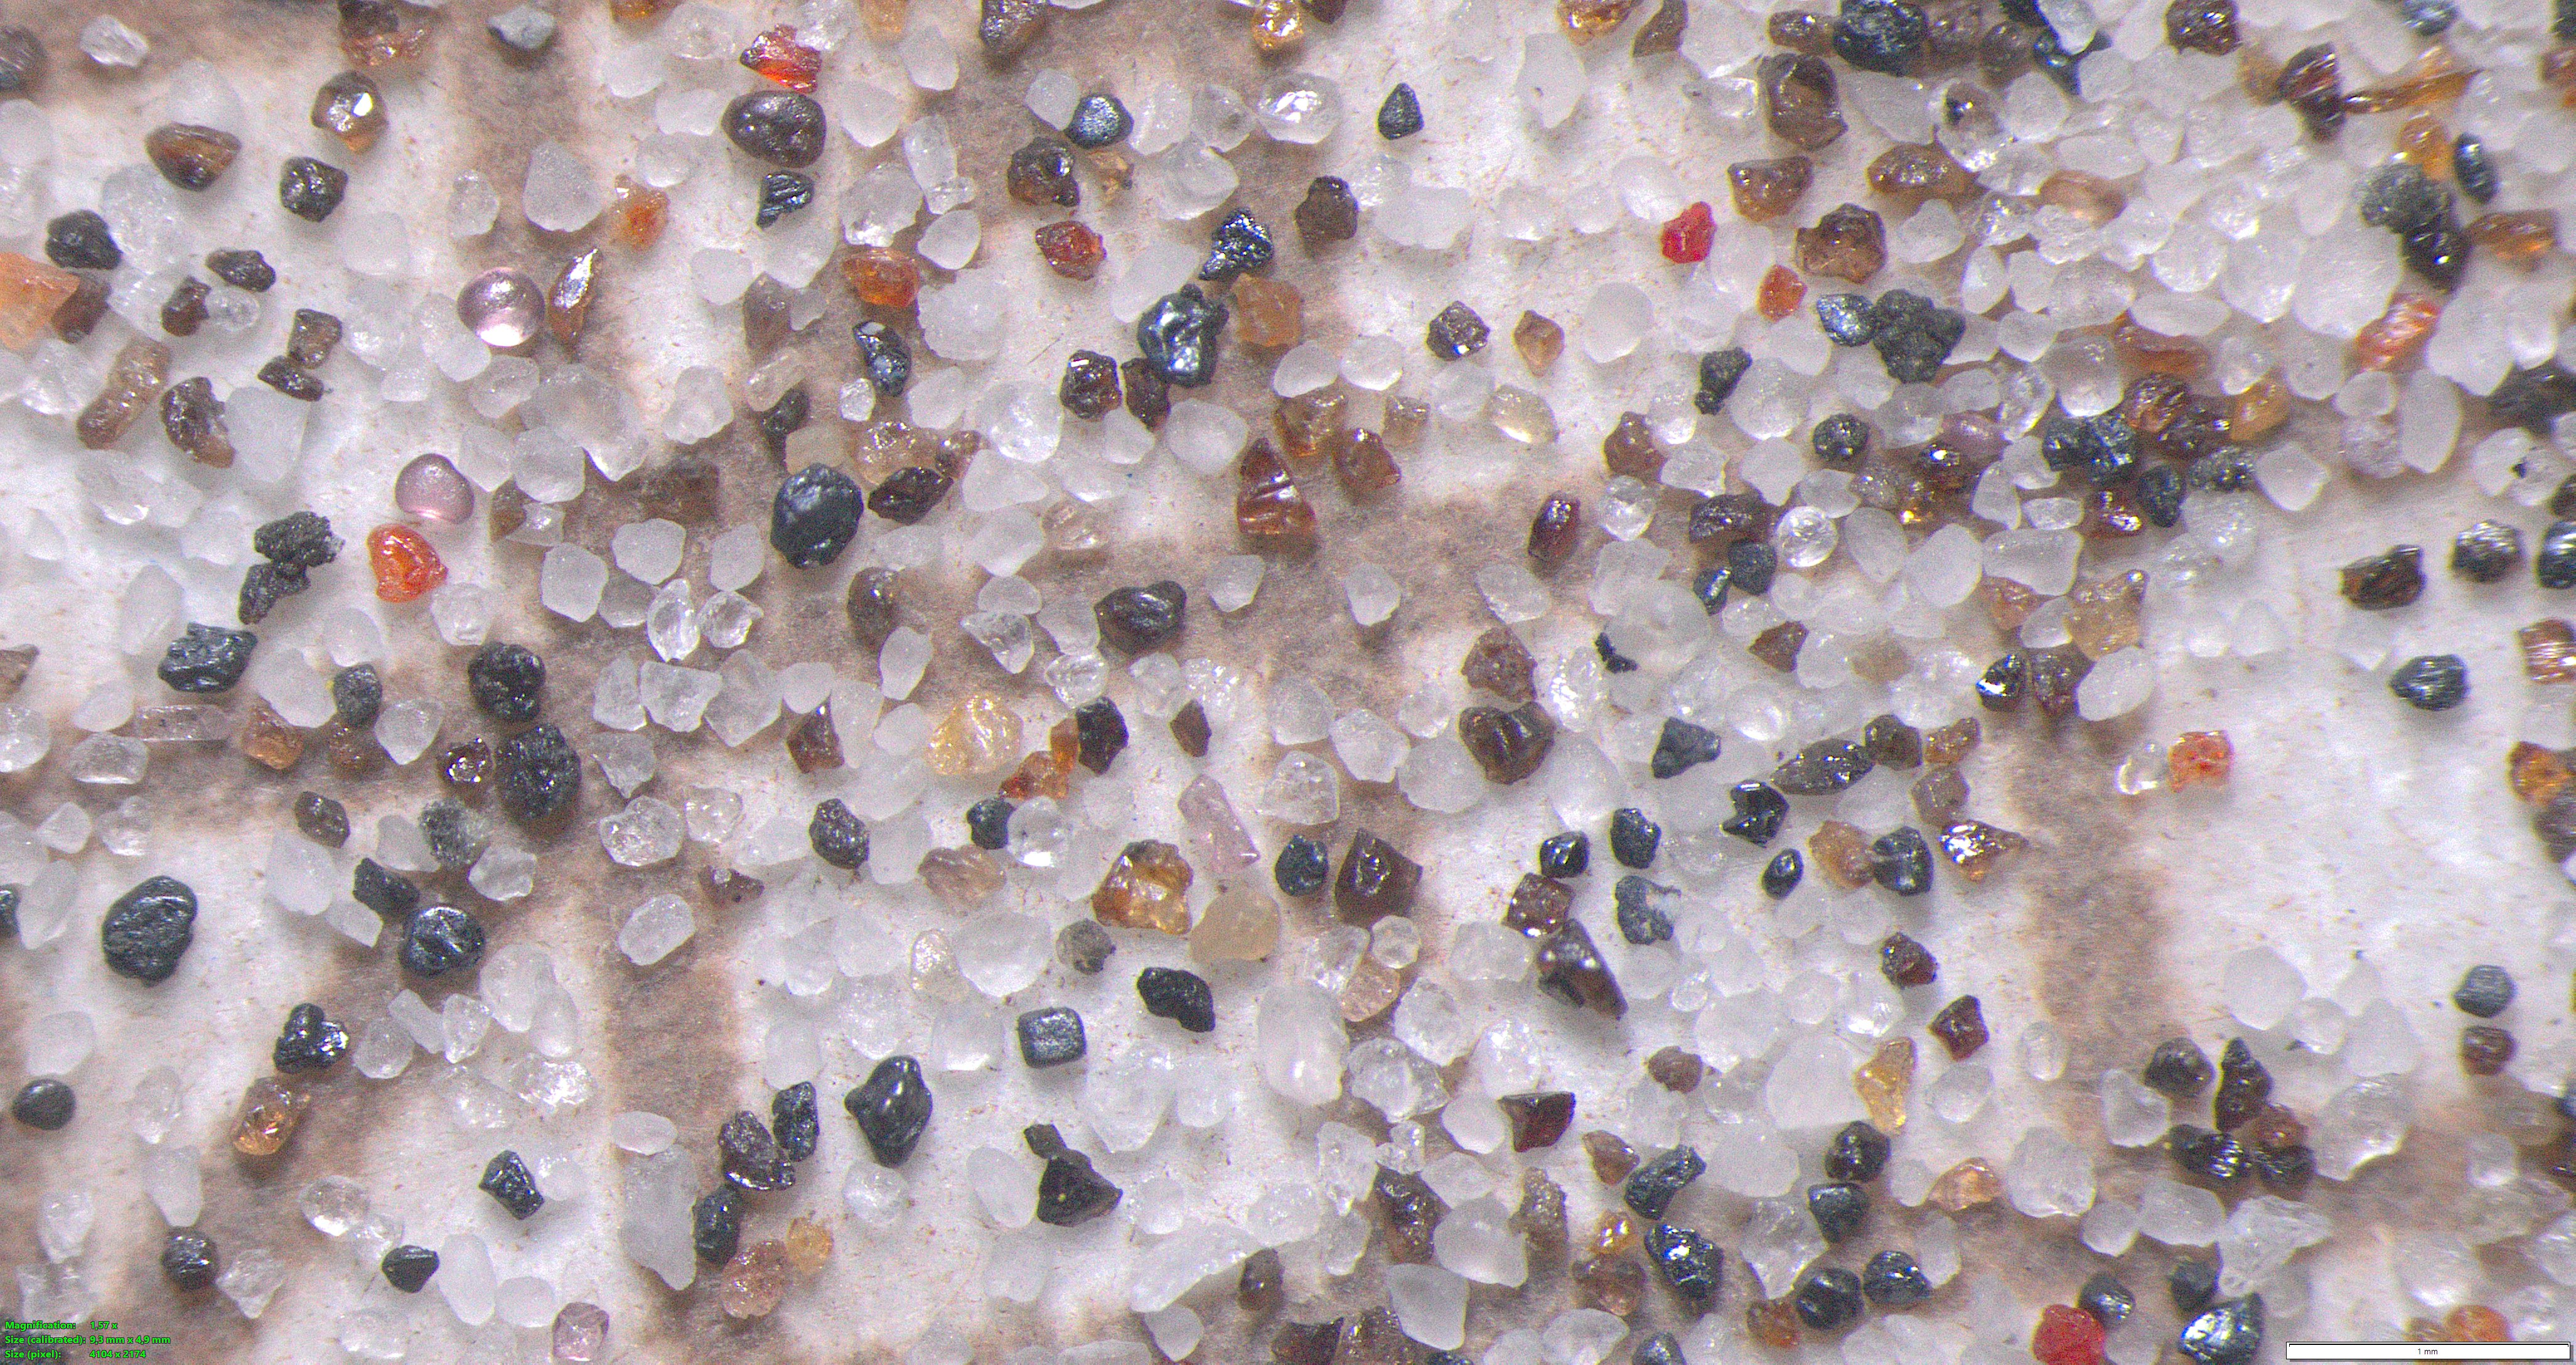
\includegraphics[width=\textwidth]{figure/sebeleumResize.jpg}
%         \caption{Citra Awal tanpa \textit{Flip}}
%         \label{fig:4.CitraAwalFlip}
%     \end{subfigure}
    
%     % Baris kedua: satu gambar di bawah tengah
%     \vskip\baselineskip
%     \begin{subfigure}[b]{0.475\textwidth}
%         \centering
%         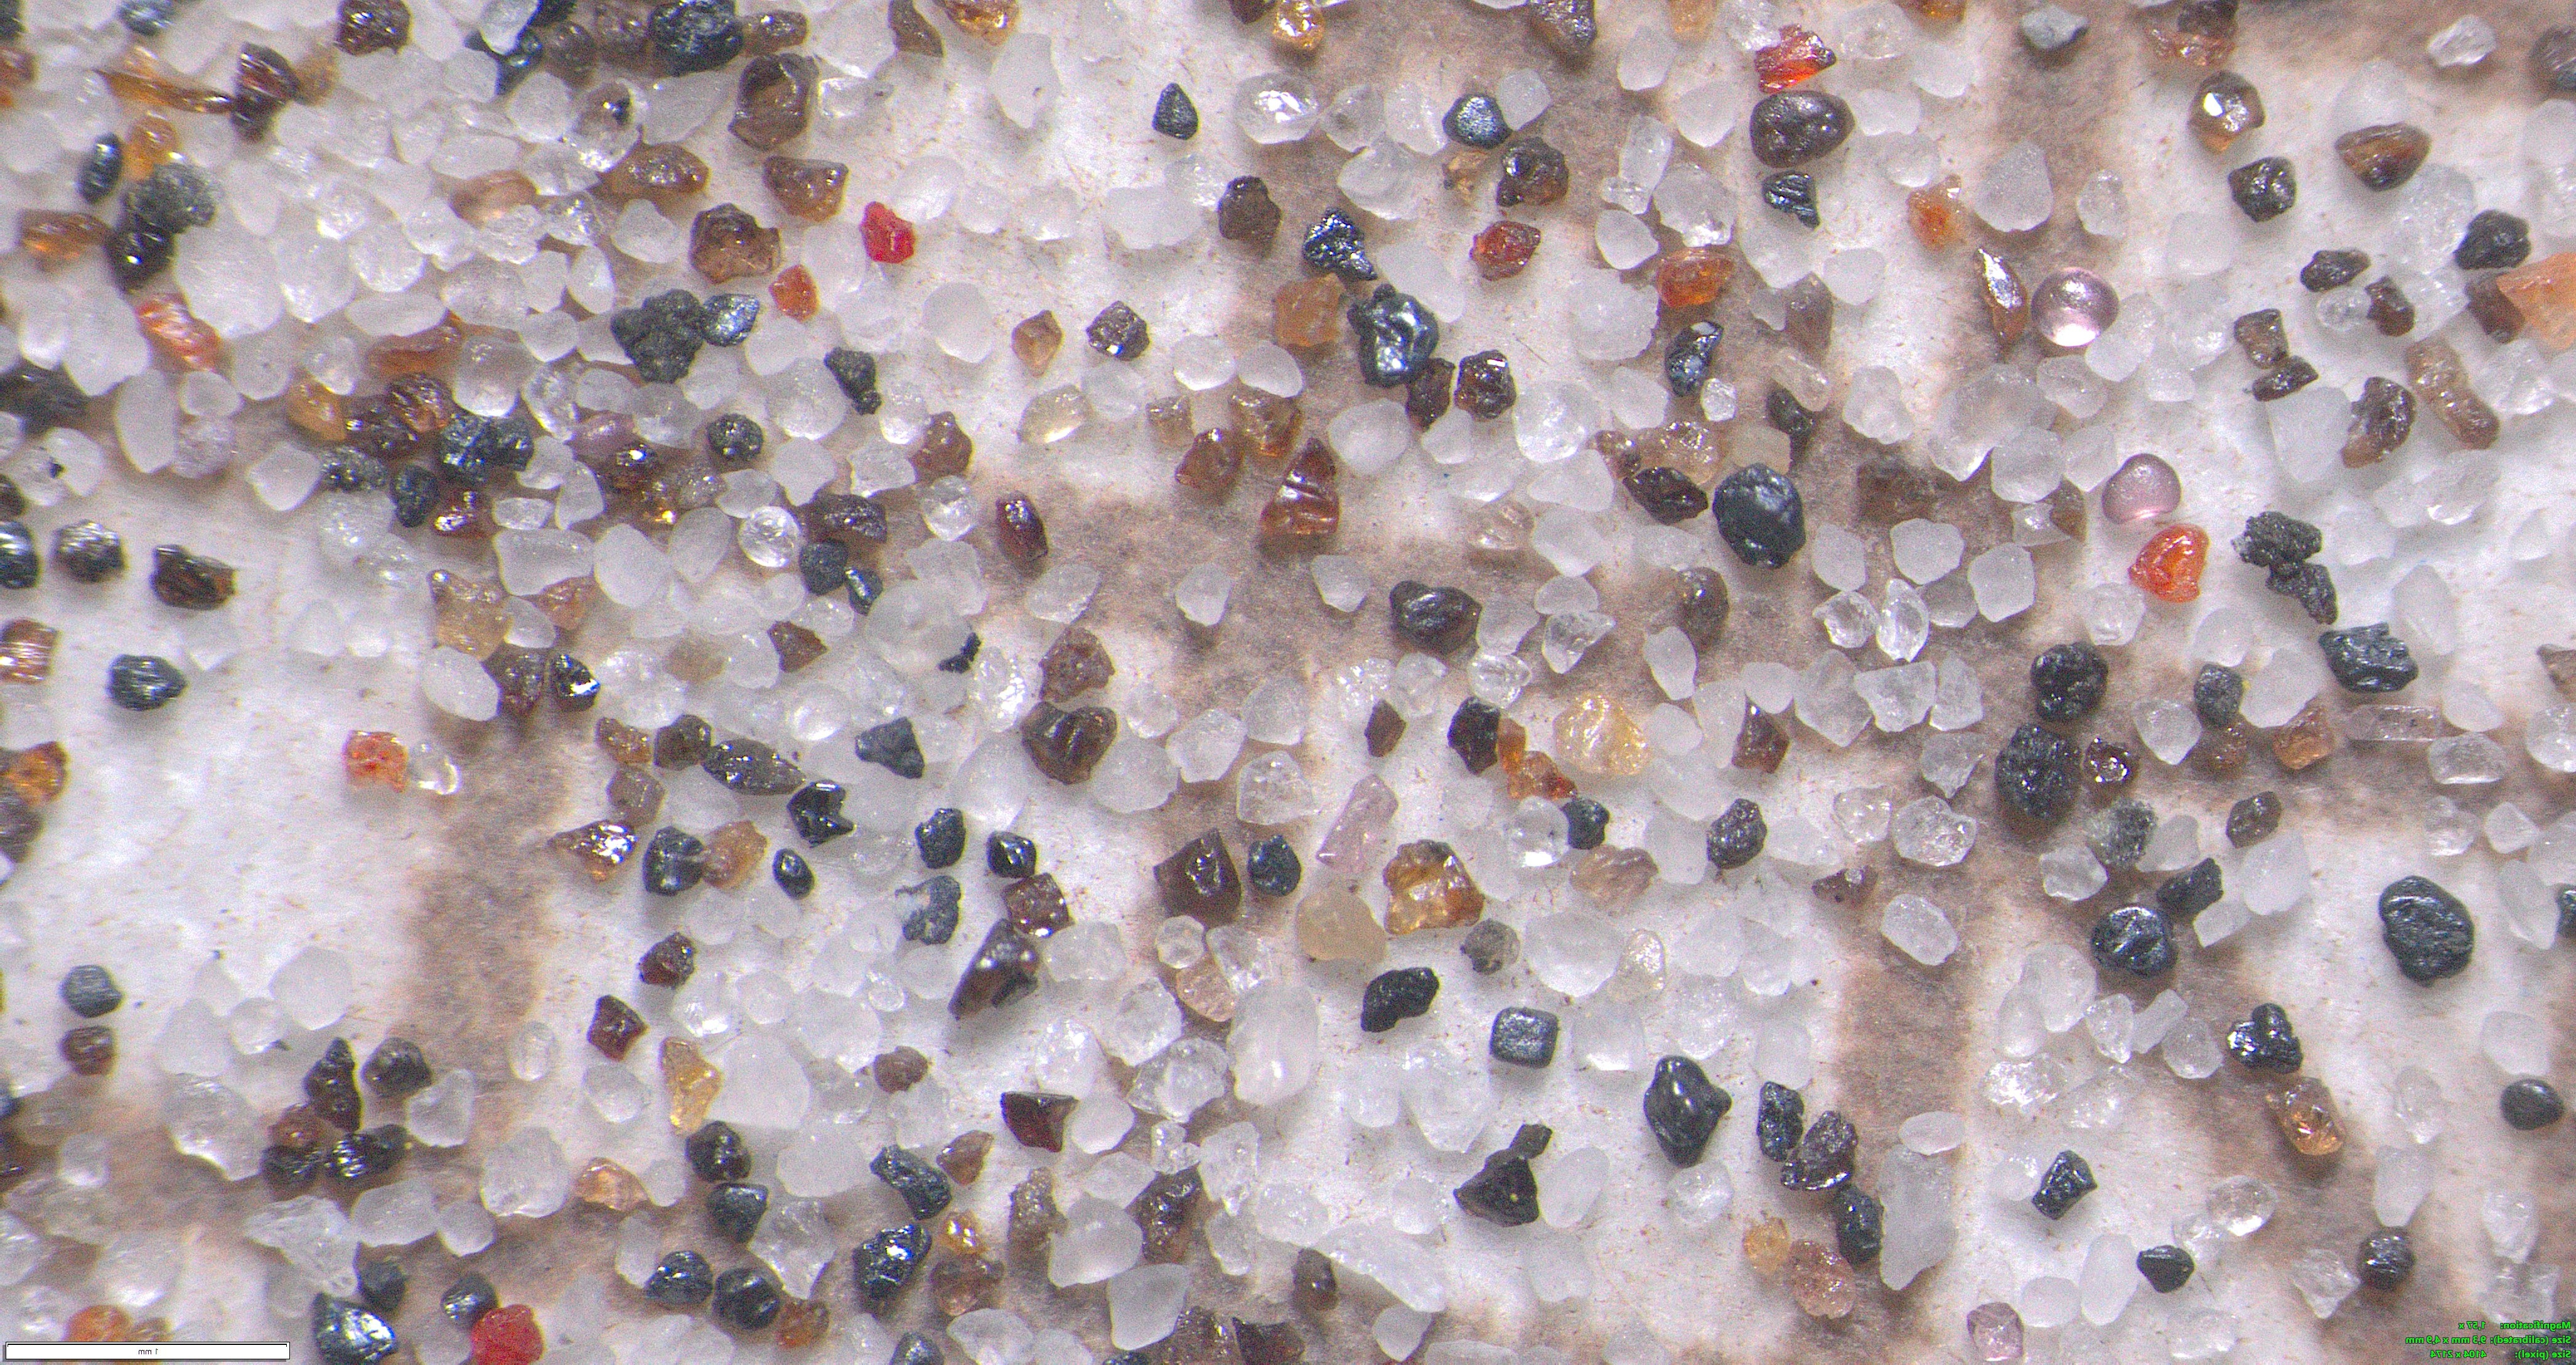
\includegraphics[width=\textwidth]{figure/hasilFlipHorizontal.jpg}
%         \caption{Hasil \textit{Flip} Horizontal ($\curvearrowright$)}
%         \label{fig:4.hasilFlipHorizontal}
%     \end{subfigure}
%     \hfill
%     \begin{subfigure}[b]{0.475\textwidth}
%         \centering
%         \includegraphics[width=\textwidth]{figure/hasilFlipVertical.jpg}
%         % \caption{Hasil \textit{Flip} Vertical ($\shortdownarrow$)}
%         \caption{Hasil \textit{Flip} Vertical (\protect$\downarrow$)}
%         % \caption{Hasil \textit{Flip} Vertical ($\downarrow$)}

%         \label{fig:4.hasilFlipVertical}
%     \end{subfigure}
%     \caption{Hasil \textit{Flip} Data}
%     \label{fig:4.HasilFlipData}
% \end{figure}

\subsubsection*{\textnormal{2. \textit{Rotate}}}
Penerapan augmentasi \textit{rotate} dilakukan menggunakan pustaka \textit{Albumentations} dengan menerapkan fungsi \texttt{A.Rotate(limit=(-15, 15), p=0.5, border\_mode=cv2.BORDER\_CONSTANT)}. Teknik ini menghasilkan variasi sudut orientasi citra kasiterit yang memperkaya data pelatihan tanpa mengubah karakteristik objek. Variasi ini menggunakan range antara -15 dan 15 derajat \texttt{(limit=(-15, 15))} dan probabilitas 0{,}5 \texttt{(p=0.5)} untuk menerapkan augmentasi. Contoh hasil \textit{rotate} ditunjukkan pada Gambar \ref{fig:3.HasilRotateData}. \par

% \begin{figure}[H]
%     \centering
%     % Baris pertama: dua gambar sejajar
%     \begin{subfigure}[b]{0.475\textwidth}
%         \centering
%         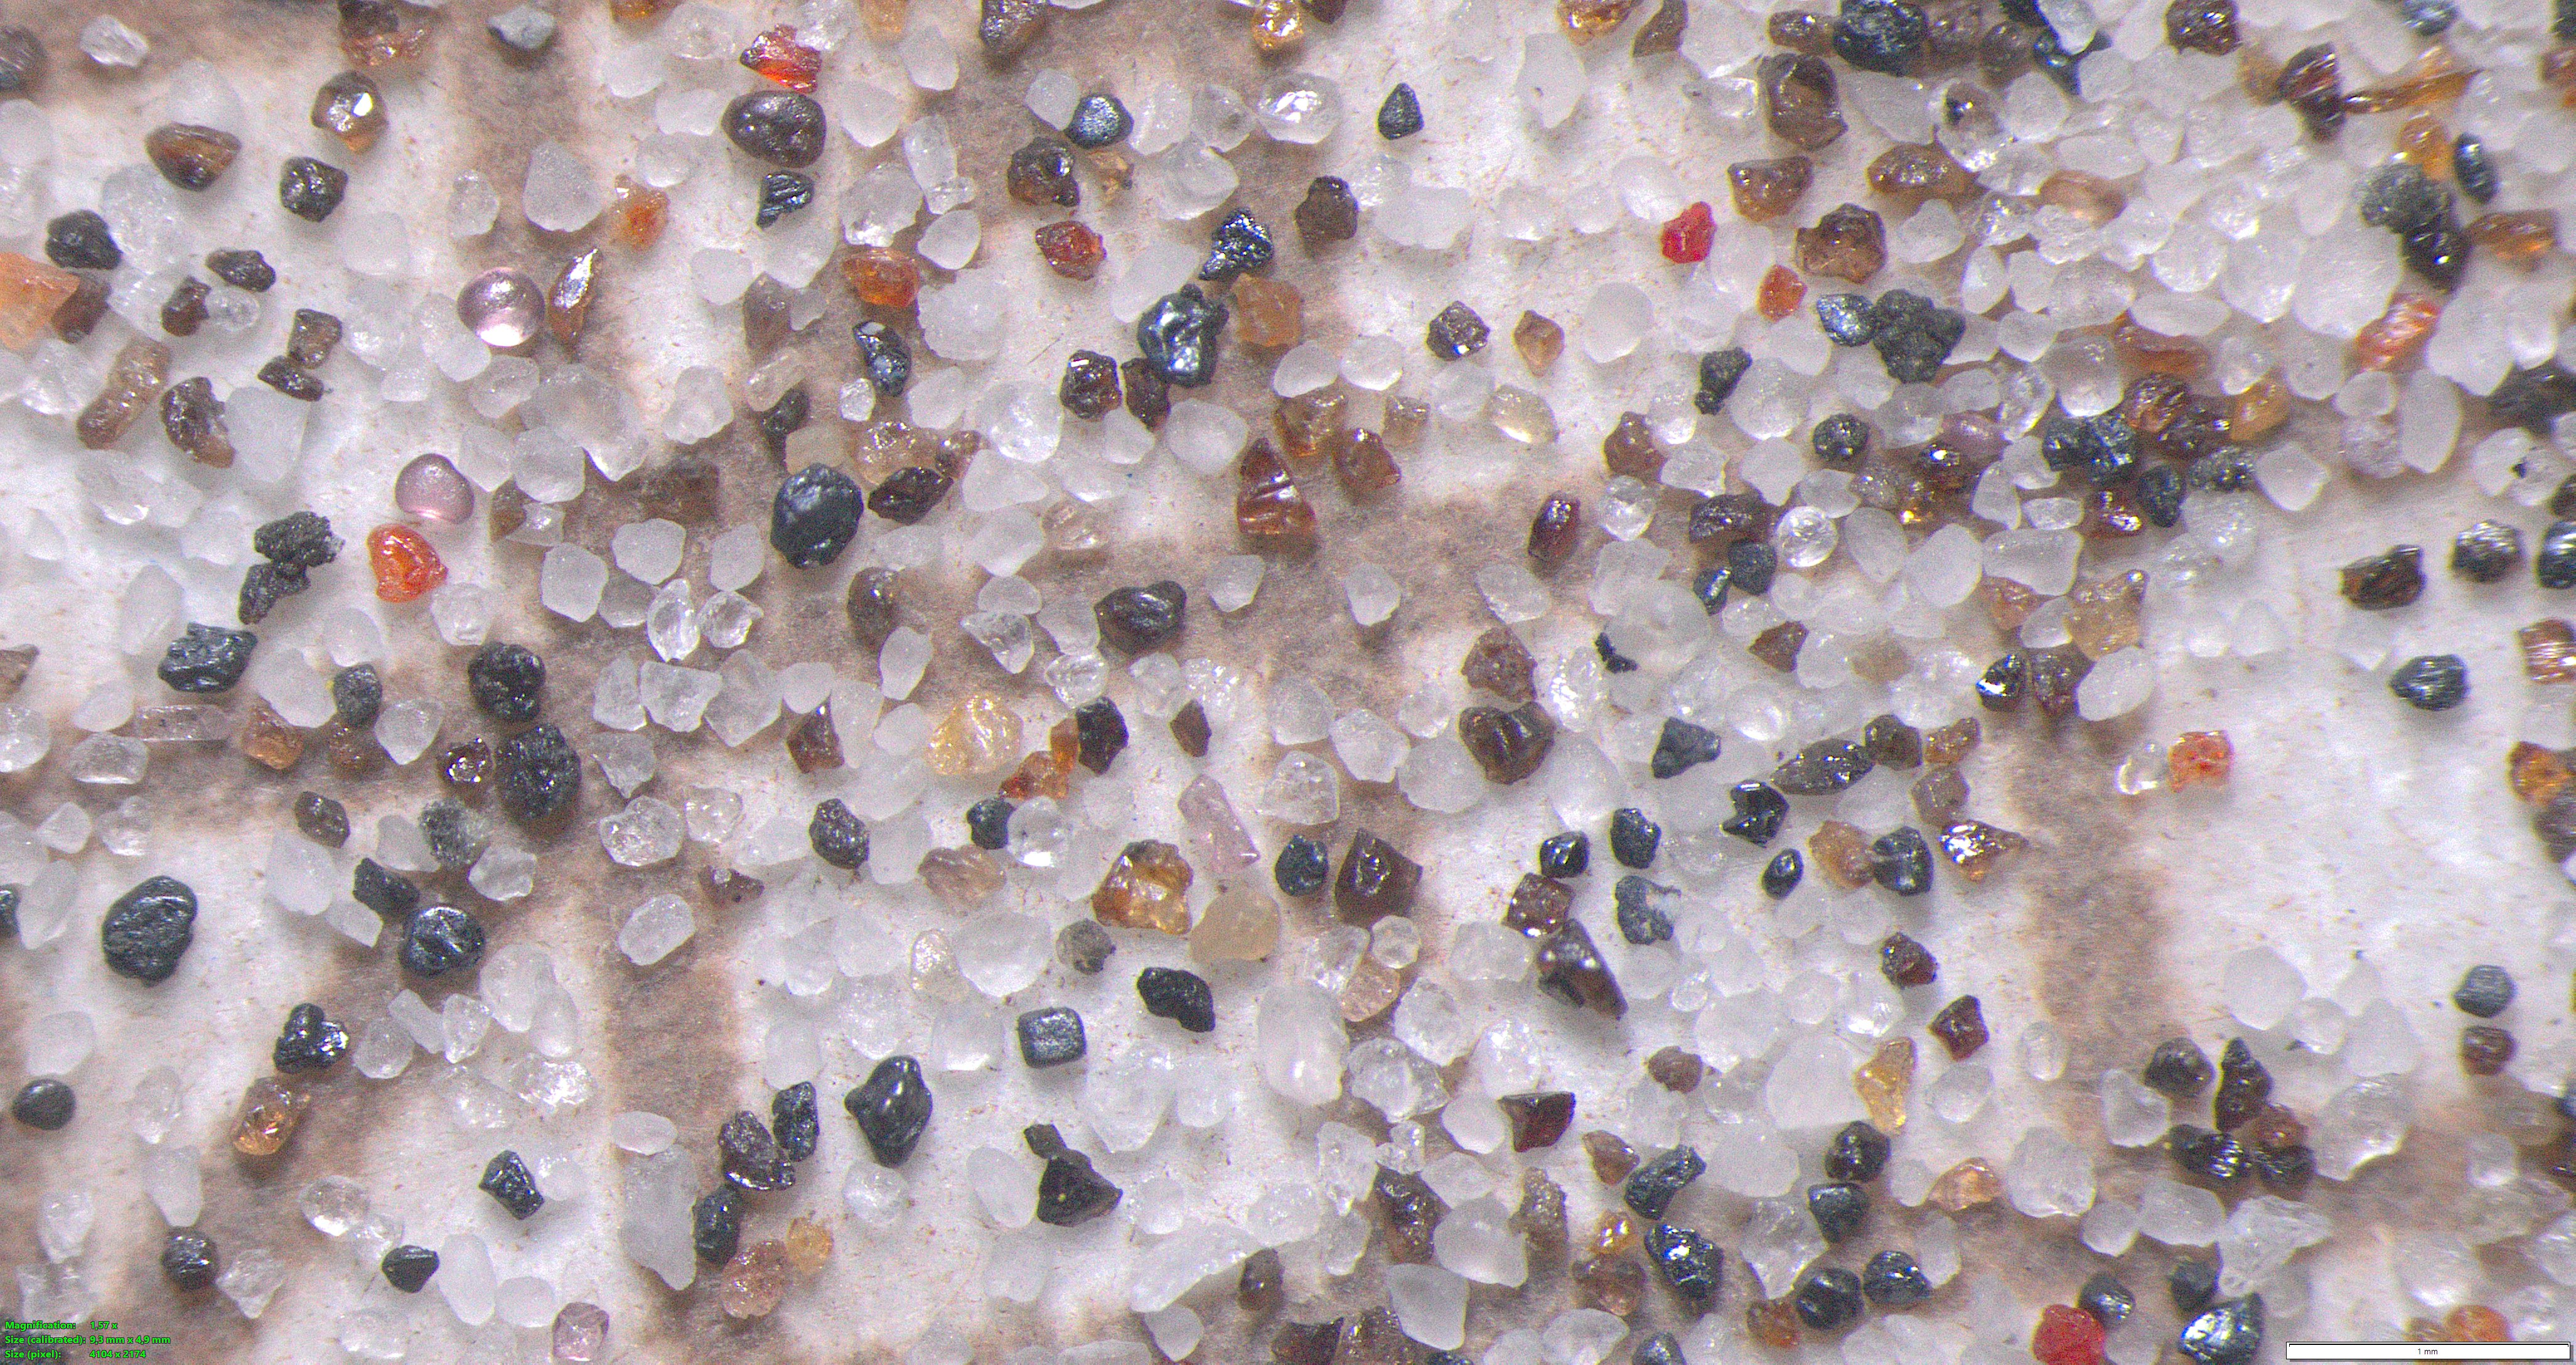
\includegraphics[width=\textwidth]{figure/sebeleumResize.jpg}
%         \caption{Citra Awal tanpa \textit{Rotate}}
%         \label{fig:4.RotateAwal}
%     \end{subfigure}
%     \hfill
%     \begin{subfigure}[b]{0.475\textwidth}
%         \centering
%         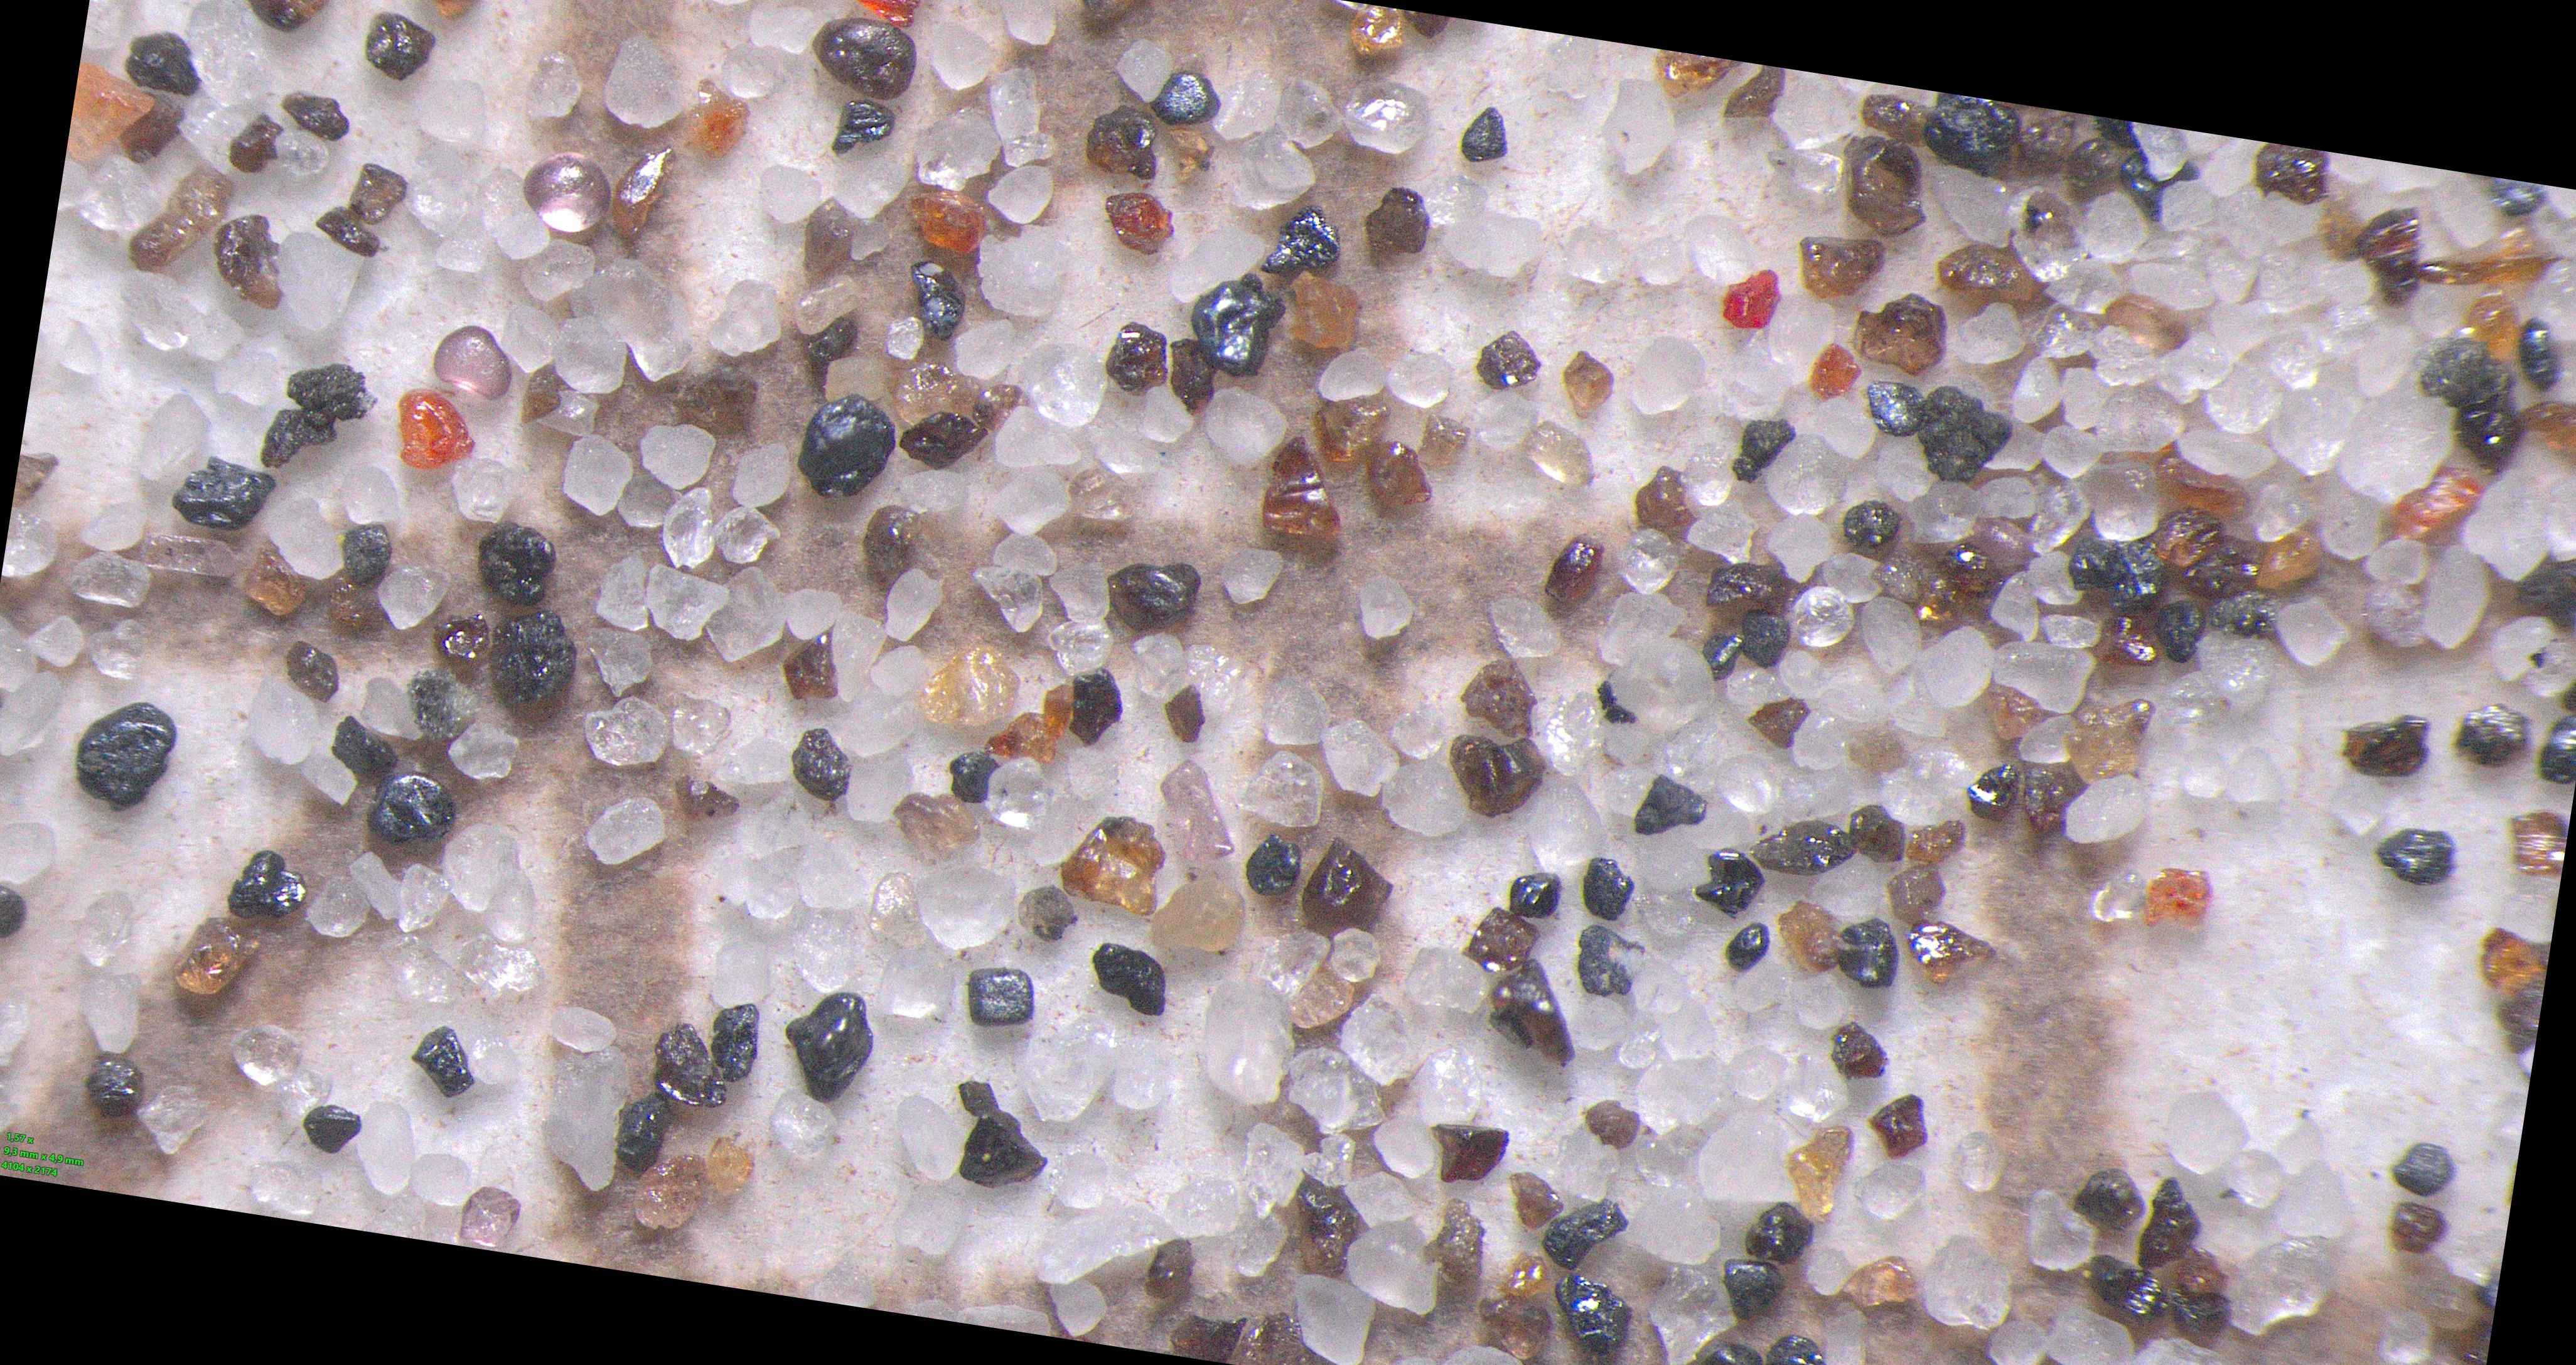
\includegraphics[width=\textwidth]{figure/hasilRotate.jpg}
%         \caption{Hasil \textit{Rotate} dengan 15\textdegree}
%         \label{fig:4.HasilRotate}
%     \end{subfigure}

% 	\caption{Hasil \textit{Rotate} Data}
%     \label{fig:4.HasilRotateData}
% \end{figure}

\subsubsection*{\textnormal{3. \textit{Gaussian Noise}}}
Penerapan augmentasi \textit{Gaussian noise} dilakukan menggunakan pustaka \textit{Albumentations} dengan menerapkan fungsi \texttt{A.GaussNoise(std\_range=(0.44721359549995793928183473374626, 0.44721359549995793928183473374626), mean\_range=(0.0, 0.0), per\_channel=True, p=0.4)}. Teknik ini menghasilkan variasi citra kasiterit dengan gangguan visual ringan tanpa mengubah struktur objek utama. Variasi ini menggunakan standar deviasi 0{,}44721359549995793928183473374626 \texttt{(std\_range=(0.44721359549995793928183473374626, 0.44721359549995793928183473374626))} yang hasilnya variansi 0{,}2 dengan perhitungan yang sudah di jelaskan pada \ref{eq:2.gaussian_distribution} dan menggunakan probabilitas 0{,}4 \texttt{(p=0.4)} untuk menerapkan augmentasi. Contoh hasil \textit{Gaussian noise} ditunjukkan pada Gambar \ref{fig:3.HasilGaussianNoiseData}. \par

% \begin{figure}[H]
%     \centering
%     % Baris pertama: dua gambar sejajar
%     \begin{subfigure}[b]{0.475\textwidth}
%         \centering
%         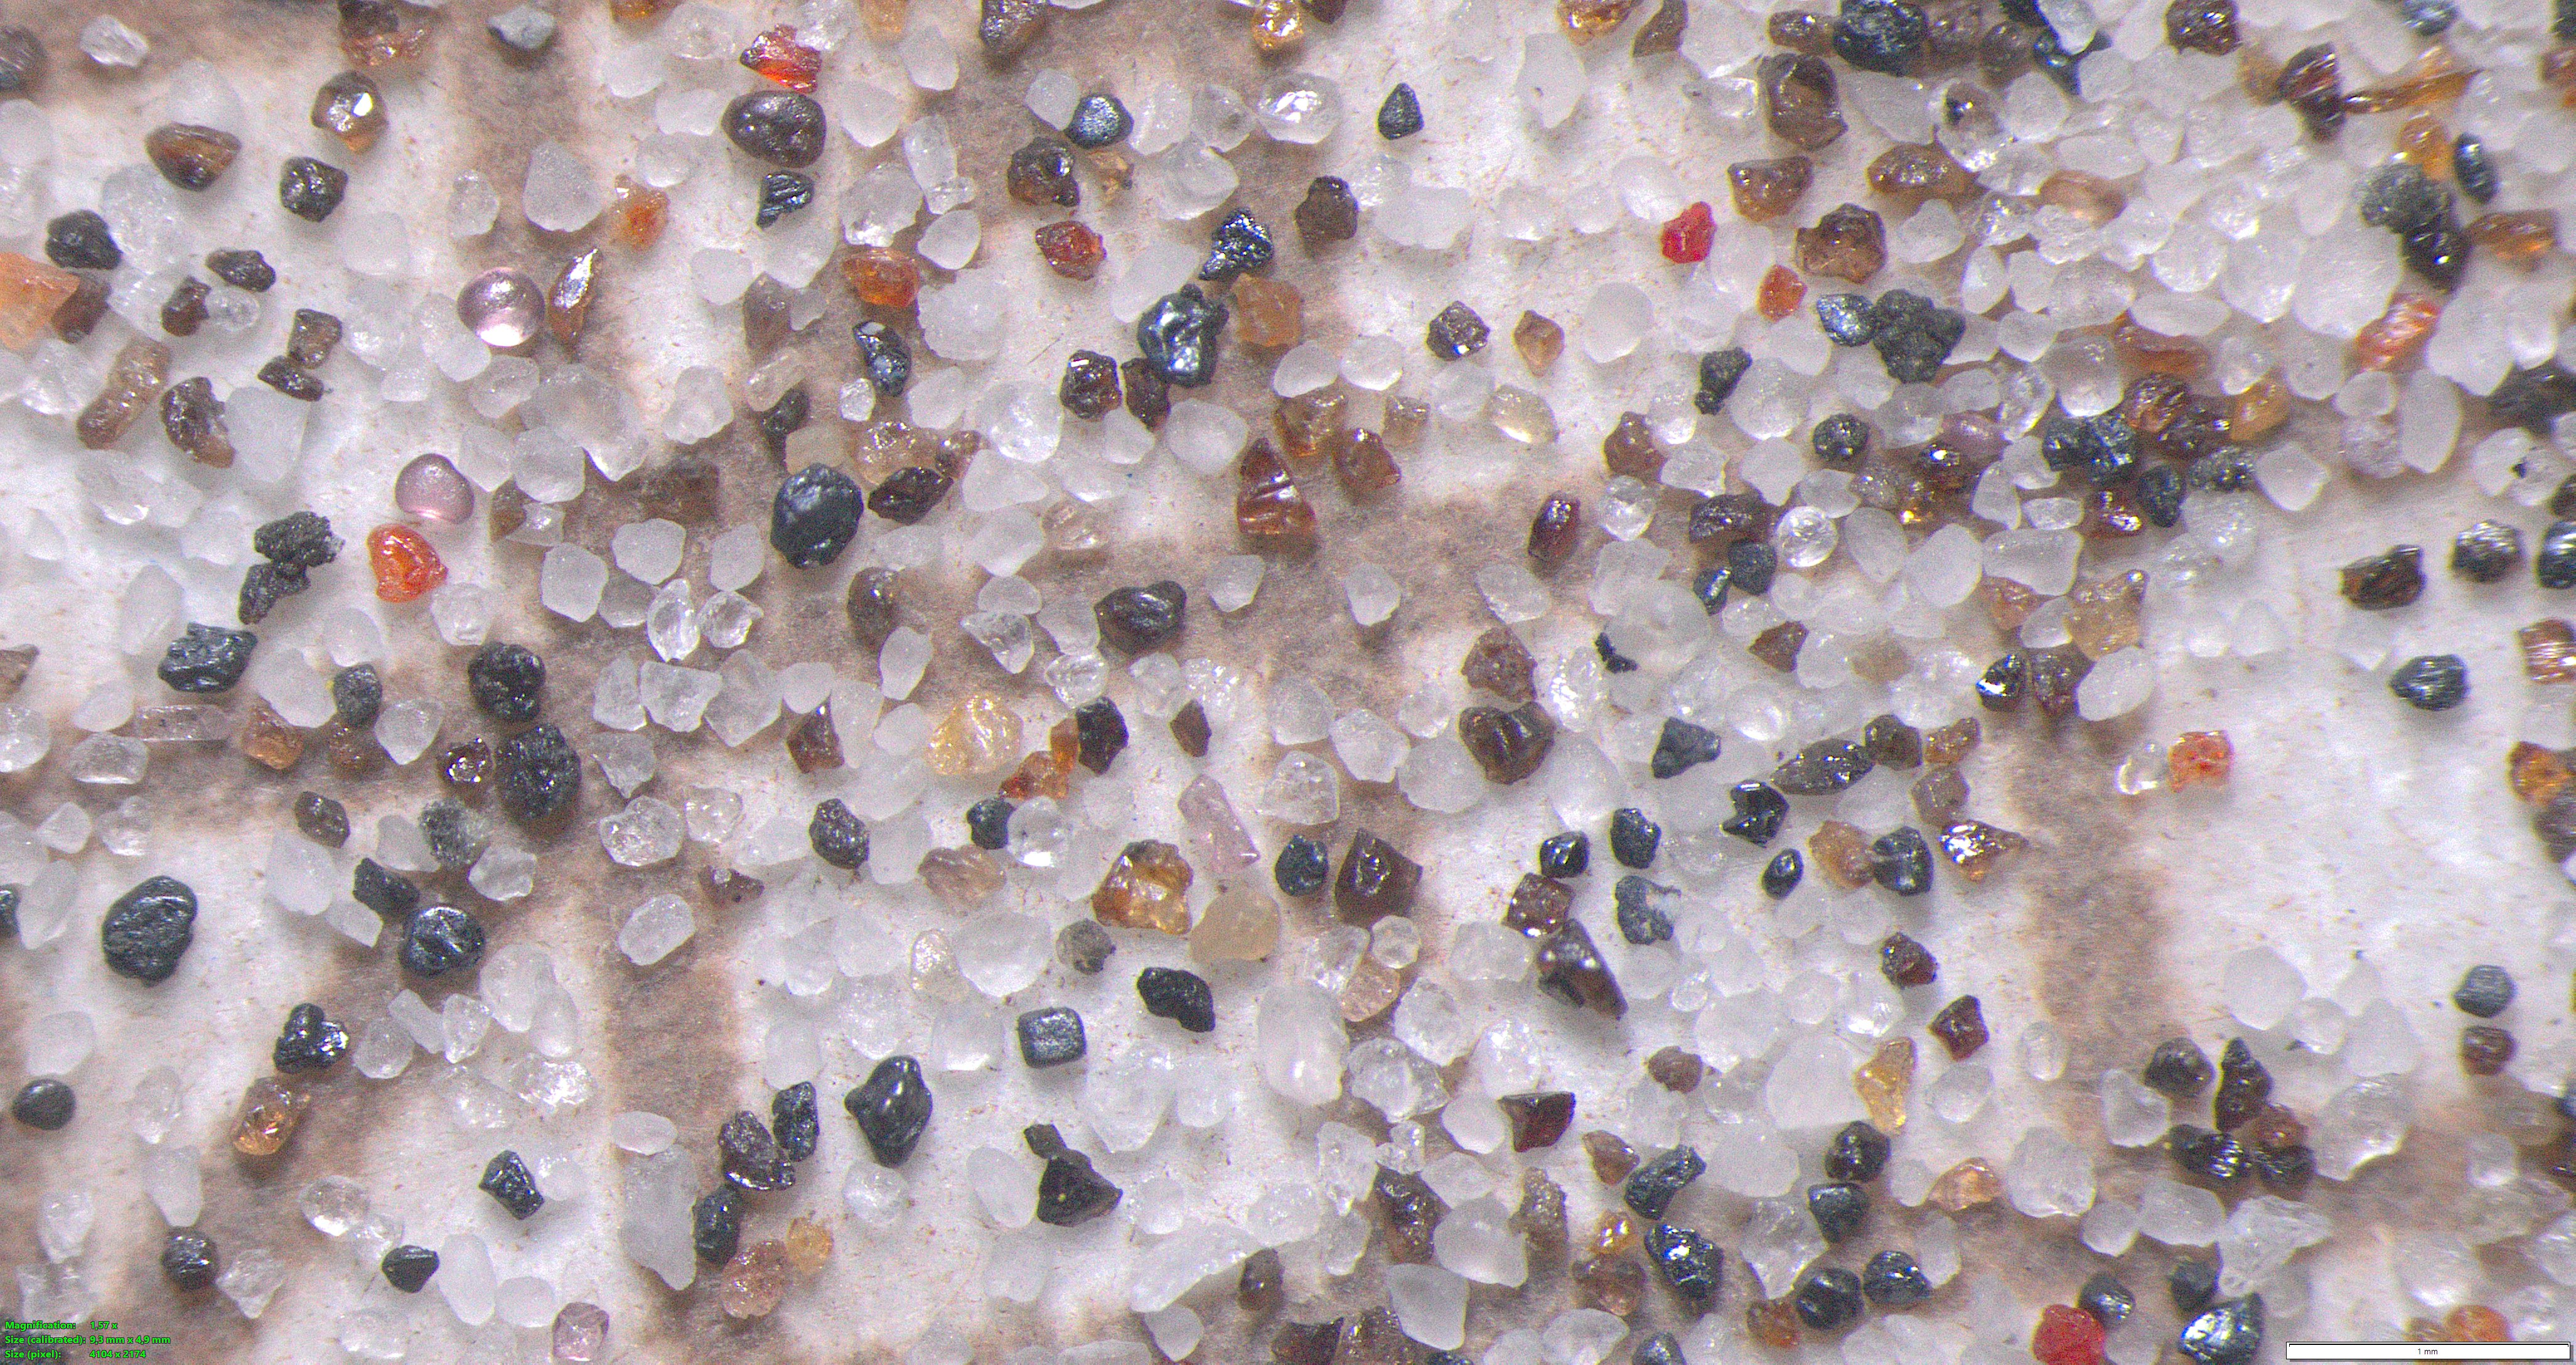
\includegraphics[width=\textwidth]{figure/sebeleumResize.jpg}
%         \caption{Citra Awal tanpa \textit{Gaussian Noise}}
%         \label{fig:4.GaussianAwal}
%     \end{subfigure}
%     \hfill
%     \begin{subfigure}[b]{0.475\textwidth}
%         \centering
%         \includegraphics[width=\textwidth]{figure/hasilGaussianNoise.jpg}
%         \caption{Hasil \textit{Gaussian Noise} dengan variansi 0{,}2}
%         \label{fig:4.HasilGaussianNoise}
%     \end{subfigure}

% 	\caption{Hasil \textit{Gaussian Noise} Data}
%     \label{fig:4.HasilGaussianNoiseData}
% \end{figure}

\subsubsection{\textit{Normalization}}
Penerapan \textit{normalization} atau normalisasi menghasilkan citra dengan rentang nilai piksel yang seragam, sehingga data pelatihan menjadi lebih stabil dan konsisten. Proses ini dilakukan dengan menggunakan nilai \textit{mean} [0{,}0, 0{,}0, 0{,}0] dan standar deviasi [1{,}0, 1{,}0, 1{,}0], sehingga nilai piksel dinormalisasi dengan rata-rata nol dan variansi satu. Kondisi ini mendukung stabilitas proses pelatihan dan meningkatkan efektivitas pembelajaran model. Kode untuk tahap augmentasi dan normalisasi dapat dilihat pada Kode \ref{code:4.code_augmentasi_normalisasi}. \par

% Menulis blok kode
\begin{lstlisting}[caption={Proses Augmentasi dan Normalisasi}, label={code:4.code_augmentasi_normalisasi}]
def get_train_transform():
    """
    Augmentasi tipis untuk training - flip, rotate, noise ringan.
    """
    return A.Compose([
        A.HorizontalFlip(p=0.4),
        A.VerticalFlip(p=0.4),
        A.Rotate(limit=(-15, 15), p=0.5, border_mode=cv2.BORDER_CONSTANT),
        A.GaussNoise(std_range=(0.44721359549995793928183473374626, 0.44721359549995793928183473374626), mean_range=(0.0, 0.0), per_channel=True, p=0.3), # Gaussian noise dengan variansi 0.2
        A.Normalize(mean=(0.0, 0.0, 0.0), std=(1.0, 1.0, 1.0), max_pixel_value=255.0),
        ToTensorV2(),
    ])


def get_val_transform():
    """
    Transformasi untuk validation - hanya normalisasi.
    """
    return A.Compose([
        A.Normalize(mean=(0.0, 0.0, 0.0), std=(1.0, 1.0, 1.0), max_pixel_value=255.0),
        ToTensorV2(),
    ])

\end{lstlisting}

Tahap augmentasi dan normalisasi citra dapat dilihat pada fungsi \texttt{get\_train\_transform()} yang digunakan untuk menerapkan augmentasi dan juga fungsi \texttt{A.Normalize()} digunakan untuk menormalisasi nilai piksel citra berdasarkan parameter \textit{mean} dan standar deviasi, sementara \texttt{ToTensorV2()} berfungsi untuk mengubah format citra menjadi \textit{tensor} agar dapat diproses oleh model PyTorch. Fungsi \texttt{get\_val\_transform()} juga menerapkan normalisasi dan konversi \textit{tensor} yang sama untuk keperluan validasi agar format data tetap konsisten. \par

\subsection{Pengembangan Model} \label{IV.Pengembangan_Model}
Pada tahap pengembangan model, dilakukan pembagian data menggunakan metode \textit{k-fold cross validation}. Selanjutnya, proses pelatihan dan evaluasi dilaksanakan pada masing-masing arsitektur model yang digunakan dalam penelitian.

\subsubsection{Pembagian Data}
Proses pembagian data dilakukan untuk memisahkan dataset menjadi data pelatihan dan data validasi. Jumlah data yang digunakan berjumlah 537 \textit{tiles}, yang terbagi ke dalam 5 \textit{fold} dengan rasio pembagian 80:20 pada setiap iterasi. Kode yang digunakan untuk proses pembagian data tersebut dapat dilihat pada Kode \ref{code:4.kfold_pembagian_data}. \par
% Menulis blok kode
\begin{lstlisting}[caption={Proses Pembagian Data}, label={code:4.kfold_pembagian_data}]
class CassiteriteDataset(Dataset):
...
    def __getitem__(self, idx):
        # Get image file and tile index
        img_name, tile_id = self.tile_index[idx]
        img_path = os.path.join(self.root_dir, img_name)
        
        # Load full image
        image = cv2.imread(img_path)
        
        if image is None:
            raise ValueError(f"Failed to load image: {img_path}")
        
        image = cv2.cvtColor(image, cv2.COLOR_BGR2RGB)
        original_h, original_w = image.shape[:2]
        
        # Load annotation
        json_name = os.path.splitext(img_name)[0] + '.json'
        json_path = os.path.join(self.root_dir, json_name)

    ...
def prepare_kfold_datasets(root_dir=ROOT_DIR, n_splits=5, grid=(2, 2)):
    """
    Mempersiapkan 5-fold cross-validation datasets dengan automatic splitting.
    """
    # Get all image files
    all_files = [f for f in os.listdir(root_dir) if f.endswith(('.jpg', '.jpeg', '.png'))]
    all_files = sorted(all_files)
    
    print(f"Total images found: {len(all_files)}")
    print(f"Grid split: {grid[0]}x{grid[1]} = {grid[0] * grid[1]} tiles per image")
    
    # Pre-compute semua valid tiles dari semua images
    print("\nPre-computing all valid tiles...")
    all_tiles = []
    for img_file in all_files:
        valid_tiles = get_valid_tiles_from_image(root_dir, img_file, grid)
        all_tiles.extend(valid_tiles)
    
    print(f"Total valid tiles: {len(all_tiles)}")
    
    # K-Fold split pada tiles
    kfold = KFold(n_splits=n_splits, shuffle=True, random_state=42)
    fold_datasets = []
    
    for fold, (train_idx, val_idx) in enumerate(kfold.split(all_tiles)):
        print(f"\nFold {fold + 1}/{n_splits}")
        
        train_tiles = [all_tiles[i] for i in train_idx]
        val_tiles = [all_tiles[i] for i in val_idx]
        
        print(f"  Train tiles: {len(train_tiles)}")
        print(f"  Val tiles: {len(val_tiles)}")
        
        # Create datasets dengan tile_list langsung
        train_dataset = CassiteriteDataset(
            root_dir=root_dir,
            tile_list=train_tiles,
            grid=grid,
            transform=get_train_transform(),
            is_train=True
        )
        
        val_dataset = CassiteriteDataset(
            root_dir=root_dir,
            tile_list=val_tiles,
            grid=grid,
            transform=get_val_transform(),
            is_train=False
        )
        
        fold_datasets.append((train_dataset, val_dataset))
    
    return fold_datasets
\end{lstlisting}

Kelas \textit{CassiteriteDataset} berfungsi untuk memuat citra dan anotasi berdasarkan indeks \textit{tile}. Metode \texttt{\_\_getitem\_\_()} melakukan pembacaan citra dalam format RGB dan pemuatan anotasi JSON yang disesuaikan secara otomatis dengan nama berkas citra, sebagaimana ditunjukkan pada baris 18 dan 19 Kode~\ref{code:4.kfold_pembagian_data}. Sementara itu, fungsi \texttt{prepare\_kfold\_datasets()} bertugas mengumpulkan seluruh \textit{tile} valid melalui \texttt{get\_valid\_tiles\_from\_image()} dan membaginya ke dalam lima \textit{fold} menggunakan metode \textit{K-Fold Cross Validation}. Dalam setiap iterasi, indeks \textit{tile} dipisahkan menjadi \textit{train\_tiles} dan \textit{val\_tiles} untuk inisialisasi objek \textit{CassiteriteDataset} dengan transformasi yang sesuai. Seluruh pasangan dataset pelatihan dan validasi kemudian disimpan dalam variabel \textit{fold\_datasets} untuk tahap pelatihan, dengan ringkasan pembagian data yang disajikan pada Tabel~\ref{table:4.pembagian_kfold}. \par

\begin{table}[H]
\centering
\caption{Ilustrasi \textit{K-Fold Cross Validation}}
\label{table:4.pembagian_kfold}
\begin{tabular}{|c|c|c|c|c|c|c|c|}
\hline
\multirow{2}{*}{\textbf{Iterasi}} & \multicolumn{5}{c|}{\textbf{\textit{K-Fold}}} & \multicolumn{2}{c|}{\textbf{Data}} \\
\cline{2-8}
& \textbf{1} & \textbf{2} & \textbf{3} & \textbf{4} & \textbf{5} & \textbf{\textit{Train}} & \textbf{\textit{Validation}} \\
\hline
1 & \cellcolor{blue!20}108 & 108 & 107 & 107 & 107 & 429 & 108 \\
\hline
2 & 108 & \cellcolor{blue!20}108 & 107 & 107 & 107 & 429 & 108 \\
\hline
3 & 108 & 108 & \cellcolor{blue!20}107 & 107 & 107 & 430 & 107 \\
\hline
4 & 108 & 108 & 107 & \cellcolor{blue!20}107 & 107 & 430 & 107 \\
\hline
5 & 108 & 108 & 107 & 107 & \cellcolor{blue!20}107 & 430 & 107 \\
\hline
\multicolumn{6}{|c|}{\textbf{Total Keseluruhan \textit{Tiles}}} & \multicolumn{2}{c|}{\textbf{537}} \\
\hline
\end{tabular}

\end{table}
Pada Tabel \ref{table:4.pembagian_kfold} terlihat bahwa dataset dibagi menjadi data pelatihan (\textit{train}) dan data validasi (\textit{validation}). Pada proses \textit{k-fold cross validation} dengan lima \textit{fold}, setiap blok berwarna biru menunjukkan \textit{fold} yang berfungsi sebagai data validasi pada iterasi ke-$n$. Sebagai contoh, pada iterasi pertama Fold 1 yang berisi 108 \textit{tiles} digunakan sebagai data validasi, sedangkan Fold 2 hingga Fold 5 berperan sebagai data pelatihan dengan total 429 \textit{tiles}. Proses ini berlanjut hingga setiap \textit{fold} mendapatkan giliran menjadi data validasi satu kali. Pada setiap iterasi, jumlah data pelatihan berkisar antara 429--430 \textit{tiles} dan data validasi sebanyak 107--108 \textit{tiles}, bergantung pada distribusi \textit{fold} yang digunakan. Secara keseluruhan, total \textit{tiles} yang digunakan dalam proses \textit{k-fold cross validation} adalah 537 \textit{tiles}. \par

\subsubsection{Pelatihan Model}
Pelatihan model akan dilakukan dengan menggunakan model \textit{pre-trained} \textit{Mask} R-CNN ResNet50 FPN V1 dan \textit{Mask} R-CNN ResNet50 FPN V2 yang sudah ada di \textit{library} PyTorch. \par

\subsubsection*{\textnormal{1. Pendefinisian model \textit{pre-trained} \textit{Mask} R-CNN ResNet50 FPN V1}}
Pada tahap ini dilakukan pendefinisian model \textit{pre-trained} \textit{Mask} R-CNN dengan \textit{backbone} ResNet50 FPN V1 yang digunakan sebagai dasar pelatihan dalam penelitian ini.

% Menulis blok kode
\begin{lstlisting}[caption={Pendefinisian Model \textit{pre-trained} \textit{Mask} R-CNN ResNet50 FPN V1}, label={code:4.definisi_v1}]
def get_maskrcnn_resnet50_fpn_v1(num_classes=2, trainable_layers=3):
    """
    Create Mask R-CNN with ResNet50 + FPN V1 pretrained on COCO.
        model: Mask R-CNN V1 with COCO pretrained weights
    """
    # Load pretrained Mask R-CNN V1 with COCO weights
    model = maskrcnn_resnet50_fpn(
        weights=MaskRCNN_ResNet50_FPN_Weights.COCO_V1,
        trainable_backbone_layers=trainable_layers
    )
    
    # Replace box predictor for custom num_classes
    in_features = model.roi_heads.box_predictor.cls_score.in_features
    model.roi_heads.box_predictor = FastRCNNPredictor(in_features, num_classes)
    
    # Replace mask predictor for custom num_classes
    in_features_mask = model.roi_heads.mask_predictor.conv5_mask.in_channels
    hidden_layer = 256
    model.roi_heads.mask_predictor = MaskRCNNPredictor(
        in_features_mask,
        hidden_layer,
        num_classes
    )
    
    return model
\end{lstlisting}

Fungsi \texttt{get\_maskrcnn\_resnet50\_fpn\_v1()} pada Kode \ref{code:4.definisi_v1} digunakan untuk membangun model \textit{Mask} R-CNN dengan \textit{backbone} ResNet50 FPN V1 yang telah dilatih sebelumnya menggunakan dataset COCO. Parameter \texttt{num\_classes=2} menentukan jumlah kelas keluaran, yaitu satu kelas untuk objek kasiterit dan satu kelas untuk latar belakang, sedangkan \texttt{trainable\_layers=3} mengatur jumlah lapisan \textit{backbone} yang dapat dilatih ulang selama proses \textit{fine-tuning}. Model dimuat dengan bobot \textit{pre-trained} melalui \texttt{MaskRCNN\_ResNet50\_FPN\_Weights.COCO\_V1}. Selanjutnya, komponen \textit{box predictor} diganti menggunakan \texttt{FastRCNNPredictor} untuk menyesuaikan jumlah fitur masukan dengan jumlah kelas yang baru, dan komponen \textit{mask predictor} diganti menggunakan \texttt{MaskRCNNPredictor} dengan jumlah \textit{hidden layer} sebanyak 256 untuk menghasilkan \textit{mask} segmentasi yang sesuai dengan jumlah kelas kustom. \par

\subsubsection*{\textnormal{2. Pendefinisian model \textit{pre-trained} \textit{Mask} R-CNN ResNet50 FPN V2}}
Pada tahap ini dilakukan pendefinisian model \textit{pre-trained} \textit{Mask} R-CNN dengan \textit{backbone} ResNet50 FPN V2 yang digunakan sebagai dasar pelatihan dalam penelitian ini.

% Menulis blok kode
\begin{lstlisting}[caption={Pendefinisian Model \textit{pre-trained} \textit{Mask} R-CNN ResNet50 FPN V2}, label={code:4.definisi_v2}]
def get_maskrcnn_resnet50_fpn_v2(num_classes=2, trainable_layers=3):
    """
    Create Mask R-CNN with ResNet50 + FPN V2 pretrained on COCO.
        model: Mask R-CNN V2 with COCO pretrained weights
    """
    # Load pretrained Mask R-CNN V2 with COCO weights
    model = maskrcnn_resnet50_fpn_v2(
        weights=MaskRCNN_ResNet50_FPN_V2_Weights.COCO_V1,
        trainable_backbone_layers=trainable_layers
    )
    
    # Replace box predictor for custom num_classes
    in_features = model.roi_heads.box_predictor.cls_score.in_features
    model.roi_heads.box_predictor = FastRCNNPredictor(in_features, num_classes)
    
    # Replace mask predictor for custom num_classes
    in_features_mask = model.roi_heads.mask_predictor.conv5_mask.in_channels
    hidden_layer = 256
    model.roi_heads.mask_predictor = MaskRCNNPredictor(
        in_features_mask,
        hidden_layer,
        num_classes
    )
    
    return model
\end{lstlisting}

Fungsi \texttt{get\_maskrcnn\_resnet50\_fpn\_v2()} pada Kode \ref{code:4.definisi_v2} digunakan untuk membangun model \textit{Mask} R-CNN dengan \textit{backbone} ResNet50 FPN V2 yang merupakan versi terbaru dengan arsitektur yang lebih optimal dibandingkan V1. Parameter \texttt{num\_classes=2} menentukan jumlah kelas keluaran untuk objek kasiterit dan latar belakang, sedangkan \texttt{trainable\_layers=3} mengatur jumlah lapisan \textit{backbone} yang dapat dilatih ulang. Model dimuat dengan bobot \textit{pre-trained} melalui \texttt{MaskRCNN\_ResNet50\_FPN\_V2\_Weights.COCO\_V1}. Serupa dengan versi V1, komponen \textit{box predictor} diganti menggunakan \texttt{FastRCNNPredictor} untuk menyesuaikan jumlah fitur masukan dengan jumlah kelas baru, dan komponen \textit{mask predictor} diganti menggunakan \texttt{MaskRCNNPredictor} dengan jumlah \textit{hidden layer} sebanyak 256 untuk menghasilkan \textit{mask} segmentasi sesuai jumlah kelas kustom. 

\subsubsection*{\textnormal{3. Proses Pelatihan Model per Epoch}}
Pada tahap ini dilakukan proses pelatihan model untuk setiap \textit{epoch} menggunakan data pelatihan pada masing-masing \textit{fold}. Proses pelatihan bertujuan untuk memperbarui bobot model secara iteratif berdasarkan nilai \textit{loss} yang dihasilkan dari prediksi dan anotasi \textit{ground truth}. \par

\begin{lstlisting}[caption={Proses Pelatihan Model per Epoch}, label={code:4.train_one_epoch}]
def train_one_epoch(model, dataloader, optimizer, device, epoch,            scheduler=None, scaler=None, use_amp=False,                     warmup_iters=0, warmup_factor=0.1, global_step=0,               base_lr=0.0001, model_type='standard'):

    model.train()
    loss_meter = AverageMeter()
    amodal_loss_meter = AverageMeter()  # Track amodal loss separately
    
    pbar = tqdm(dataloader, desc=f'Epoch {epoch}')
    
    for batch_idx, (images, targets) in enumerate(pbar):
        try:
            # Clear cache before processing batch
            if batch_idx > 0:
                torch.cuda.empty_cache()
            
            # Move to device
            images = [img.to(device) for img in images]
            targets = [{k: v.to(device) for k, v in t.items()} for t in targets]
            
            # Manual warmup (avoid scheduler warning)
            if global_step < warmup_iters:
                alpha = global_step / warmup_iters
                warmup_lr = warmup_factor * (1 - alpha) + alpha
                for param_group in optimizer.param_groups:
                    param_group['lr'] = base_lr * warmup_lr
            
            # Forward pass with optional AMP
            if use_amp and scaler is not None:
                with torch.amp.autocast(device_type='cuda', dtype=torch.float16):
                    loss_dict = model(images, targets)
                    losses = sum(loss for loss in loss_dict.values())
                
                optimizer.zero_grad()
                scaler.scale(losses).backward()
                scaler.unscale_(optimizer)
                torch.nn.utils.clip_grad_norm_(model.parameters(), max_norm=10.0)
                scaler.step(optimizer)
                scaler.update()
            else:
                loss_dict = model(images, targets)
                losses = sum(loss for loss in loss_dict.values())
                optimizer.zero_grad()
                losses.backward()
                torch.nn.utils.clip_grad_norm_(model.parameters(), max_norm=10.0)
                optimizer.step()

            global_step += 1
            
            # Update metrics
            loss_meter.update(losses.item(), len(images))
            
            # Track amodal loss separately for amodal models
            if model_type == 'amodal' and 'loss_amodal_mask' in loss_dict:
                amodal_loss_meter.update(loss_dict['loss_amodal_mask'].item(), len(images))
                pbar.set_postfix({
                    'loss': f'{loss_meter.avg:.4f}',
                    'amodal': f'{amodal_loss_meter.avg:.4f}'
                })
            else:
                pbar.set_postfix({'loss': f'{loss_meter.avg:.4f}'})
            
            # Delete tensors to free memory
            del images, targets, loss_dict, losses
            if batch_idx % 10 == 0:  # More aggressive cache clearing
                torch.cuda.empty_cache()
...
    # Return amodal loss if available
    amodal_loss = amodal_loss_meter.avg if amodal_loss_meter.count > 0 else None
    return loss_meter.avg, global_step, amodal_loss
\end{lstlisting}

Fungsi \texttt{train\_one\_epoch()} pada Kode \ref{code:4.train_one_epoch} menunjukkan proses pelatihan model untuk satu \textit{epoch} dengan menggunakan data pelatihan yang dimuat melalui \texttt{dataloader}. Model diatur pada mode \texttt{model.train()} untuk menghitung nilai \textit{loss} berdasarkan keluaran prediksi dan anotasi, kemudian dilakukan proses \textit{backpropagation} untuk memperbarui bobot model menggunakan \texttt{optimizer} yang telah ditentukan. Untuk menjaga stabilitas pelatihan, diterapkan mekanisme \textit{learning rate warm-up} pada tahap awal iterasi serta \textit{gradient clipping} menggunakan \texttt{clip\_grad\_norm\_} untuk mencegah gradien berlebih. Nilai \textit{loss} rata-rata pada setiap \textit{epoch} dicatat menggunakan \texttt{loss\_meter}, sedangkan pada model \textit{amodal} nilai \texttt{loss\_amodal\_mask} juga dipantau secara terpisah melalui \texttt{amodal\_loss\_meter}. \par

\subsubsection*{\textnormal{4. Pelatihan Model \textit{K-Fold Cross-Validation}}}
Pada tahap ini, pelatihan model dilakukan dengan menerapkan metode \textit{k-fold cross-validation}. Fungsi \texttt{train\_one\_epoch()} dipanggil secara iteratif untuk melatih model pada setiap \textit{epoch} menggunakan data pelatihan dari masing-masing \textit{fold}.

\begin{lstlisting}[caption={Proses Pelatihan Model dengan \textit{K-Fold Cross-Validation}}, label={code:4.train_kfold}]
def train_kfold(config):
...
    # Prepare K-Fold datasets
    print("\nPreparing K-Fold datasets...")
    fold_datasets = prepare_kfold_datasets(
        root_dir=config['data_dir'],
        n_splits=config['n_folds']
    )
    
    all_fold_results = []
    total_training_start = time.time()
    
    # Train each fold
    for fold_idx, (train_dataset, val_dataset) in enumerate(fold_datasets):
        fold_num = fold_idx + 1
...
        fold_start_time = time.time()
        
        # Create model configuration directory name
        lr_str = f"{config['lr']:.0e}" if config['lr'] < 0.01 else f"{config['lr']}"
        model_config_dir = f"{config['backbone']}_{config['model_type']}
         _{config['optimizer']}_lr{lr_str}"
...
        # Create fold directory inside configuration directory
        fold_dir = os.path.join(config_output_dir, f'fold{fold_num}')
        os.makedirs(fold_dir, exist_ok=True)
        
        # DataLoaders
        train_loader = get_dataloader(
            train_dataset,
            batch_size=config['batch_size'],
            shuffle=True,
            num_workers=config['num_workers']
        )
        
        val_loader = get_dataloader(
            val_dataset,
            batch_size=config['batch_size'],
            shuffle=False,
            num_workers=config['num_workers']
        )
        
        # Create model
        print(f"Creating {config['model_type']} model...")
        model = get_model(
            num_classes=config['num_classes'],
            model_type=config['model_type'],
            backbone=config['backbone'],
            trainable_layers=config['trainable_layers']
        )
        model = model.to(device)
        count_parameters(model)
        
        # Optimizer
        params = [p for p in model.parameters() if p.requires_grad]
        if config['optimizer'] == 'sgd':
            optimizer = optim.SGD(
                params, 
                lr=config['lr'], 
                momentum=config.get('momentum', 0.9),
                weight_decay=config['weight_decay']
            )
        elif config['optimizer'] == 'adam':
            optimizer = optim.Adam(
                params, 
                lr=config['lr'], 
                weight_decay=config['weight_decay']
            )
...
        # Main scheduler: CosineAnnealingWarmRestarts
        scheduler = CosineAnnealingWarmRestarts(
            optimizer, 
            T_0=config.get('COSINE_T0', 20),
            T_mult=config.get('COSINE_T_MULT', 1),
            eta_min=config.get('COSINE_ETA_MIN', 1e-6)
        )
        
        # Warmup parameters (manual warmup untuk avoid warning)
        warmup_iters = min(1000, len(train_loader))
        warmup_factor = 0.1
        
        # GradScaler
        use_amp = config.get('use_amp', False)
        scaler = torch.amp.GradScaler(device='cuda', enabled=use_amp)
        
        # Early stopping
        early_stopping = EarlyStopping(
            patience=config.get('early_stopping_patience', 3),
            min_delta=0.0001,
            mode='max',
            verbose=True
        )
...
        best_ap = 0.0  # Track best AP@0.50:0.95 (PRIMARY METRIC)
        best_epoch = 0
        global_step = 0  # Track global step for warmup
        
        for epoch in range(1, config['epochs'] + 1): # Training loop
            print(f"\n--- Epoch {epoch}/{config['epochs']} ---")
            start_time = time.time()

            # Train
            train_loss, global_step, amodal_loss = train_one_epoch(
                model, train_loader, optimizer, device, epoch,
                scheduler=scheduler,
                scaler=scaler,
                use_amp=use_amp,
                warmup_iters=warmup_iters,
                warmup_factor=warmup_factor,
                global_step=global_step,
                base_lr=config['lr'],
                model_type=config['model_type']
            )
            
            # Validate with COCO 2025 metrics
            val_results = validate(model, val_loader, device, use_amp=use_amp, model_type=config['model_type'])
            scheduler.step()
            epoch_time = time.time() - start_time

            val_loss = val_results['val_loss']
            ap_50_95 = val_results['AP@0.50:0.95']  # PRIMARY METRIC      
\end{lstlisting}
Fungsi \texttt{train\_kfold()} pada Kode \ref{code:4.train_kfold} mengimplementasikan alur pelatihan model menggunakan metode \textit{k-fold cross-validation}. Proses diawali dengan pembagian dataset melalui \texttt{prepare\_kfold\_datasets()} sesuai jumlah \textit{fold} yang ditentukan. Pada setiap iterasi \textit{fold}, data dimuat menggunakan \texttt{get\_dataloader()} dan arsitektur model dibangun melalui fungsi \texttt{get\_model()}. Optimasi bobot dilakukan menggunakan \texttt{optim.SGD} atau \texttt{optim.Adam}. Pengaturan laju pembelajaran dikelola secara adaptif menggunakan \texttt{CosineAnnealingWarmRestarts}. Di dalam \textit{training loop}, fungsi \texttt{train\_one\_epoch()} dipanggil untuk memperbarui parameter model, diikuti oleh fungsi \texttt{validate()} untuk mengevaluasi performa pada data validasi. Dengan demikian, pada setiap \textit{fold}, proses pelatihan model dilakukan selama sejumlah \textit{epoch} yang telah ditentukan, di mana pada setiap \textit{epoch} fungsi \texttt{train\_one\_epoch()} dipanggil untuk memperbarui parameter model menggunakan data pelatihan pada \textit{fold} tersebut. Hasil evaluasi berupa \texttt{AP@0.50:0.95} digunakan sebagai metrik untuk menentukan model terbaik, yang juga dipantau oleh mekanisme \texttt{EarlyStopping} guna mencegah \textit{overfitting}. \par

\subsubsection*{\textnormal{5. Evaluasi Model}}
Pada tahap evaluasi, model yang telah dilatih diuji menggunakan data validasi untuk mengukur kemampuan deteksi dan segmentasi objek kasiterit. Evaluasi dilakukan untuk menilai kesesuaian prediksi model terhadap \textit{ground truth} secara kuantitatif menggunakan metrik standar \textit{COCO}, sehingga kinerja model dapat dianalisis secara objektif dan terukur.

% Menulis blok kode
\begin{lstlisting}[caption={Proses Evaluasi Model}, label={code:4.evaluasi_validate}]
@torch.no_grad()
def validate(model, dataloader, device, use_amp=False,                        model_type='standard'):

    model.eval()
    loss_meter = AverageMeter()
    amodal_loss_meter = AverageMeter()  # Track amodal loss for validation
    
    all_predictions = []
    all_targets = []
    
    pbar = tqdm(dataloader, desc='Validation')
    
    for batch_idx, (images, targets) in enumerate(pbar):
        images = [img.to(device) for img in images]
        targets = [{k: v.to(device) for k, v in t.items()} for t in targets]
        
        # Compute loss
        model.train()
        if use_amp:
            with torch.amp.autocast(device_type='cuda', dtype=torch.float16):
                loss_dict = model(images, targets)
                losses = sum(loss for loss in loss_dict.values())
        else:
            loss_dict = model(images, targets)
            losses = sum(loss for loss in loss_dict.values())
        model.eval()
        
        loss_meter.update(losses.item(), len(images))
        
        # Track amodal loss separately for amodal models
        if model_type == 'amodal' and 'loss_amodal_mask' in loss_dict:
            amodal_loss_meter.update(loss_dict['loss_amodal_mask'].item(), len(images))
        
        # Get predictions
        if use_amp:
            with torch.amp.autocast(device_type='cuda', dtype=torch.float16):
                predictions = model(images)
        else:
            predictions = model(images)
            
        all_predictions.extend(predictions)
        all_targets.extend(targets)
        
        pbar.set_postfix({'val_loss': f'{loss_meter.avg:.4f}'})
        
        # Clean up memory
        del images, targets, loss_dict, losses, predictions
        if batch_idx % 10 == 0:
            torch.cuda.empty_cache()
    
    # Use low score_threshold (0.05) to capture early training detections
    eval_metrics = calculate_batch_iou_map(all_predictions, all_targets, score_threshold=0.05)
    
    # Return dictionary with COCO-compliant keys
    results = {
        'val_loss': loss_meter.avg,
        
        # PRIMARY METRIC (wajib bold di Table 1)
        'AP@0.50:0.95': eval_metrics['AP@0.50:0.95'],
        
        # Secondary AP metrics
        'AP@0.50': eval_metrics['AP@0.50'],
        'AP@0.75': eval_metrics['AP@0.75'],
        
        # IoU metrics (modern standard)
        'IoU@0.50:0.95': eval_metrics['IoU@0.50:0.95'],
        'IoU@0.50': eval_metrics['IoU@0.50'],
        'IoU@0.75': eval_metrics['IoU@0.75'],
    }
    
    # Add validation amodal loss if available
    if amodal_loss_meter.count > 0:
        results['val_loss_amodal'] = amodal_loss_meter.avg
    
    return results
\end{lstlisting}
Hasil evaluasi yang diperoleh melalui implementasi pada Kode~\ref{code:4.contoh} menunjukkan performa model dalam memproses data validasi dengan menghitung \texttt{val\_loss} serta metrik standar \textit{COCO}. Proses ini mengagregasi \texttt{all\_predictions} dan \texttt{all\_targets} untuk kemudian diproses oleh fungsi \texttt{calculate\_batch\_iou\_map} dengan \texttt{score\_threshold} sebesar 0.05. Hasil akhir yang disimpan dalam \textit{dictionary} \texttt{results} mencakup metrik utama \texttt{AP@0.50:0.95} dan \texttt{IoU@0.50:0.95}, yang memberikan gambaran komprehensif mengenai tingkat presisi dan kesesuaian segmentasi model secara aktual. Capaian metrik tersebut menjadi basis data hasil penelitian untuk membandingkan efektivitas berbagai variasi konfigurasi model yang telah diuji.

\subsubsection*{\textnormal{6. Argument Parser Pelatihan Model}}
Setelah kedua model pre-trained sudah didefinisikan, selanjutnya dilakukan pelatihan dan evaluasi pada masing-masing model. Variasi konfigurasi pelatihan yang digunakan untuk pelatihan model dapat dilihat pada Tabel \ref{table:3.konfigurasi-model}. Argument parser yang digunakan untuk melakukan pelatihan model adalah sebagai berikut: 

\begin{enumerate}  % [label=(\alph*)]
\item \textit{Mask} R-CNN ResNet50 FPN V1 + \textit{Amodal} + SGD \smallskip
\begin{lstlisting}
python train.py --data_dir dataset142 --backbone resnet50_fpn_v1 --model_type amodal --optimizer sgd --batch_size 1 --no_amp --num_workers 14 
\end{lstlisting}
\medskip

\item \textit{Mask} R-CNN ResNet50 FPN V1 + \textit{Amodal} + \textit{Adam} \smallskip
\begin{lstlisting}
python train.py --data_dir dataset142 --backbone resnet50_fpn_v1 --model_type amodal --optimizer adam --batch_size 1 --no_amp --num_workers 14 
\end{lstlisting}
\medskip

\item \textit{Mask} R-CNN ResNet50 FPN V1 + \textit{Standard} + SGD \smallskip
\begin{lstlisting}
python train.py --data_dir dataset142 --backbone resnet50_fpn_v1 --model_type standard --optimizer sgd --batch_size 1 --no_amp --num_workers 14 
\end{lstlisting}
\medskip

\item \textit{Mask} R-CNN ResNet50 FPN V1 + \textit{Standard} + \textit{Adam} \smallskip
\begin{lstlisting}
python train.py --data_dir dataset142 --backbone resnet50_fpn_v1 --model_type standard --optimizer adam --batch_size 1 --no_amp --num_workers 14 
\end{lstlisting}
\medskip

\item \textit{Mask} R-CNN ResNet50 FPN V2 + \textit{Amodal} + SGD \smallskip
\begin{lstlisting}
python train.py --data_dir dataset142 --backbone resnet50_fpn_v2 --model_type amodal --optimizer sgd --batch_size 1 --no_amp --num_workers 14 
\end{lstlisting}
\medskip

\item \textit{Mask} R-CNN ResNet50 FPN V2 + \textit{Amodal} + \textit{Adam} \smallskip
\begin{lstlisting}
python train.py --data_dir dataset142 --backbone resnet50_fpn_v2 --model_type amodal --optimizer adam --batch_size 1 --no_amp --num_workers 14 
\end{lstlisting}
\medskip

\item \textit{Mask} R-CNN ResNet50 FPN V2 + \textit{Standard} + SGD \smallskip
\begin{lstlisting}
python train.py --data_dir dataset142 --backbone resnet50_fpn_v2 --model_type standard  --optimizer sgd --batch_size 1 --no_amp --num_workers 14 
\end{lstlisting}
\medskip

\item \textit{Mask} R-CNN ResNet50 FPN V2 + \textit{Standard} + \textit{Adam} \smallskip
\begin{lstlisting}
python train.py --data_dir dataset142 --backbone resnet50_fpn_v2 --model_type standard --optimizer adam --batch_size 1 --no_amp --num_workers 14 
\end{lstlisting}
\end{enumerate}

% \begin{lstlisting}
% python train.py --data_dir dataset142 --backbone resnet50_fpn_v1 --model_type amodal --optimizer sgd --lr 1e-2 --batch_size 1 --no_amp --num_workers 14 --COSINE_ETA_MIN 1e-4
% \end{lstlisting}
% \medskip

% \item \textit{Mask} R-CNN ResNet50 FPN V1 + \textit{Amodal} + \textit{Adam} \smallskip
% \begin{lstlisting}
% python train.py --data_dir dataset142 --backbone resnet50_fpn_v1 --model_type amodal --optimizer adam --lr 1e-4 --batch_size 1 --weight_decay 1e-5 --no_amp --num_workers 14 
% \end{lstlisting}
% \medskip

% \item \textit{Mask} R-CNN ResNet50 FPN V1 + \textit{Standard} + SGD \smallskip
% \begin{lstlisting}
% python train.py --data_dir dataset142 --backbone resnet50_fpn_v1 --model_type standard --optimizer sgd --lr 1e-2 --batch_size 1 --no_amp --num_workers 14 --COSINE_ETA_MIN 1e-4
% \end{lstlisting}
% \medskip

% \item \textit{Mask} R-CNN ResNet50 FPN V1 + \textit{Standard} + \textit{Adam} \smallskip
% \begin{lstlisting}
% python train.py --data_dir dataset142 --backbone resnet50_fpn_v1 --model_type standard --optimizer adam --lr 1e-4 --batch_size 1 --weight_decay 1e-5 --no_amp --num_workers 14 
% \end{lstlisting}
% \medskip

% \item \textit{Mask} R-CNN ResNet50 FPN V2 + \textit{Amodal} + SGD \smallskip
% \begin{lstlisting}
% python train.py --data_dir dataset142 --backbone resnet50_fpn_v2 --model_type amodal --optimizer sgd --lr 1e-2 --batch_size 1 --no_amp --num_workers 14 --COSINE_ETA_MIN 1e-4
% \end{lstlisting}
% \medskip

% \item \textit{Mask} R-CNN ResNet50 FPN V2 + \textit{Amodal} + \textit{Adam} \smallskip
% \begin{lstlisting}
% python train.py --data_dir dataset142 --backbone resnet50_fpn_v2 --model_type amodal --optimizer adam --lr 1e-4 --batch_size 1 --weight_decay 1e-5 --no_amp --num_workers 14 
% \end{lstlisting}
% \medskip

% \item \textit{Mask} R-CNN ResNet50 FPN V2 + \textit{Standard} + SGD \smallskip
% \begin{lstlisting}
% python train.py --data_dir dataset142 --backbone resnet50_fpn_v2 --model_type standard  --optimizer sgd --lr 1e-2 --batch_size 1 --no_amp --num_workers 14 --COSINE_ETA_MIN 1e-4
% \end{lstlisting}
% \medskip

% \item \textit{Mask} R-CNN ResNet50 FPN V2 + \textit{Standard} + \textit{Adam} \smallskip
% \begin{lstlisting}
% python train.py --data_dir dataset142 --backbone resnet50_fpn_v2 --model_type standard --optimizer adam --lr 1e-4 --batch_size 1 --weight_decay 1e-5 --no_amp --num_workers 14 
% \end{lstlisting}
% \end{enumerate}

\section{Hasil Evaluasi} \label{IV.Hasil_Evaluasi}
Berdasarkan hasil evaluasi yang telah dilakukan, hasil evaluasi ditampilkan berdasarkan dua \textit{Model Pre-trained} dari arsitektur \textit{Mask} R-CNN yakni \textit{Mask} R-CNN ResNet50 FPN V1 dan \textit{Mask} R-CNN ResNet50 FPN V2. Evaluasi dilakukan menggunakan metrik \textit{Average Precision} (AP) dan \textit{Intersection over Union} (IoU) pada beberapa ambang batas, yaitu \textit{0.5}, \textit{0.75}, dan \textit{0.5:0.95} dengan metrik evaluasi utama yang digunakan adalah \textit{AP50:95} dan \textit{IoU50:95} karena mampu merepresentasikan kinerja model secara lebih menyeluruh pada berbagai tingkat ketelitian deteksi. Evaluasi dilakukan dengan skema \textit{k-fold cross validation} pada beberapa variasi konfigurasi pelatihan meliputi model \textit{Amodal} dan \textit{Standard} serta \textit{optimizer} SGD dan \textit{Adam}. \par

\subsection{Hasil Evaluasi \textit{Mask} R-CNN ResNet50 FPN V1}
Hasil evaluasi \textit{Model Pre-trained} \textit{Mask} R-CNN ResNet50 FPN V1 dengan variasi konfigurasi pelatihan dan dihitung metrik AP dan IoU ditampilkan pada Tabel \ref{table:4.hasil_evaluasi_model_v1}.

\begin{table}[H]
\centering
\caption{Hasil Evaluasi \textit{Mask} R-CNN ResNet50 FPN V1}
\label{table:4.hasil_evaluasi_model_v1}
% \footnotesize
\small
% \setlength{\tabcolsep}{6pt} % Menyesuaikan jarak antar kolom agar lebih ramping
\makebox[\textwidth][c]{
\begin{tabular}{|c|c|c|c|c|c|c|c|c|c|}
\hline
\multirow{2}{*}{\textbf{No}} & \multirow{2}{*}{\textbf{Model}} & \multirow{2}{*}{\textbf{Optim}} & \multirow{2}{*}{\textbf{Fold}} & \multicolumn{3}{c|}{\textbf{AP}} & \multicolumn{3}{c|}{\textbf{IoU}} \\
\cline{5-10}
& & & & \textbf{0.5} & \textbf{0.75} & \textbf{0.5:0.95} & \textbf{0.5} & \textbf{0.75} & \textbf{0.5:0.95} \\
\hline
\multirow{6}{*}{1} & \multirow{6}{*}{\textit{Amodal}} & \multirow{6}{*}{SGD} & 1 & 0{,}571 & 0{,}524 & 0{,}468 & 0{,}889 & 0{,}909 & 0{,}911 \\
\cline{4-10}
& & & 2 & 0{,}554 & 0{,}524 & 0{,}462 & 0{,}896 & 0{,}915 & 0{,}918 \\
\cline{4-10}
& & & 3 & 0{,}519 & 0{,}478 & 0{,}423 & 0{,}887 & 0{,}906 & 0{,}910 \\
\cline{4-10}
& & & 4 & 0{,}537 & 0{,}503 & 0{,}449 & 0{,}899 & 0{,}916 & \textbf{0{,}919} \\
\cline{4-10}
& & & 5 & 0{,}525 & 0{,}491 & 0{,}430 & 0{,}889 & 0{,}907 & 0{,}911 \\
\cline{4-10}
& & & Avg & 0{,}541 & 0{,}504 & 0{,}446 & 0{,}892 & 0{,}911 & 0{,}914 \\
\hline
\multirow{6}{*}{2} & \multirow{6}{*}{\textit{Amodal}} & \multirow{6}{*}{\textit{Adam}} & 1 & 0{,}589 & 0{,}540 & \textbf{0{,}487} & 0{,}890 & 0{,}913 & 0{,}915 \\
\cline{4-10}
& & & 2 & 0{,}550 & 0{,}514 & 0{,}455 & 0{,}894 & 0{,}914 & 0{,}916 \\
\cline{4-10}
& & & 3 & 0{,}538 & 0{,}493 & 0{,}446 & 0{,}893 & 0{,}913 & 0{,}915 \\
\cline{4-10}
& & & 4 & 0{,}549 & 0{,}515 & 0{,}456 & 0{,}896 & 0{,}912 & 0{,}915 \\
\cline{4-10}
& & & 5 & 0{,}544 & 0{,}509 & 0{,}445 & 0{,}890 & 0{,}909 & 0{,}913 \\
\cline{4-10}
& & & \cellcolor{black!15}Avg & 0{,}554 & 0{,}514 & \cellcolor{black!15}\textbf{0{,}458} & 0{,}893 & 0{,}912 & \cellcolor{black!15}\textbf{0{,}915} \\
\hline
\multirow{6}{*}{3} & \multirow{6}{*}{\textit{Standard}} & \multirow{6}{*}{SGD} & 1 & 0{,}572 & 0{,}531 & 0{,}462 & 0{,}886 & 0{,}904 & 0{,}908 \\
\cline{4-10}
& & & 2 & 0{,}533 & 0{,}497 & 0{,}431 & 0{,}885 & 0{,}905 & 0{,}909 \\
\cline{4-10}
& & & 3 & 0{,}526 & 0{,}489 & 0{,}423 & 0{,}882 & 0{,}899 & 0{,}904 \\
\cline{4-10}
& & & 4 & 0{,}536 & 0{,}508 & 0{,}448 & 0{,}897 & 0{,}914 & 0{,}917 \\
\cline{4-10}
& & & 5 & 0{,}518 & 0{,}484 & 0{,}422 & 0{,}888 & 0{,}908 & 0{,}912 \\
\cline{4-10}
& & & Avg & 0{,}537 & 0{,}502 & 0{,}437 & 0{,}888 & 0{,}906 & 0{,}910 \\
\hline
\multirow{6}{*}{4} & \multirow{6}{*}{\textit{Standard}} & \multirow{6}{*}{\textit{Adam}} & 1 & 0{,}586 & 0{,}542 & 0{,}477 & 0{,}887 & 0{,}909 & 0{,}912 \\
\cline{4-10}
& & & 2 & 0{,}554 & 0{,}521 & 0{,}454 & 0{,}886 & 0{,}908 & 0{,}912 \\
\cline{4-10}
& & & 3 & 0{,}533 & 0{,}489 & 0{,}435 & 0{,}888 & 0{,}907 & 0{,}911 \\
\cline{4-10}
& & & 4 & 0{,}547 & 0{,}509 & 0{,}451 & 0{,}890 & 0{,}911 & 0{,}913 \\
\cline{4-10}
& & & 5 & 0{,}530 & 0{,}494 & 0{,}431 & 0{,}889 & 0{,}907 & 0{,}911 \\
\cline{4-10}
& & & Avg & 0{,}536 & 0{,}499 & 0{,}450 & 0{,}888 & 0{,}908 & 0{,}912 \\
\hline
\end{tabular}
}
\end{table}

Visualisasi dari hasil evaluasi \textit{Mask} R-CNN ResNet50 FPN V1 ditampilkan pada Gambar \ref{fig:4.hasil_evaluasi_model_v1}.

\begin{figure}[H] % Kalau menggunakan H, posisi gambar akan tepat dibawah teks
    \centering
    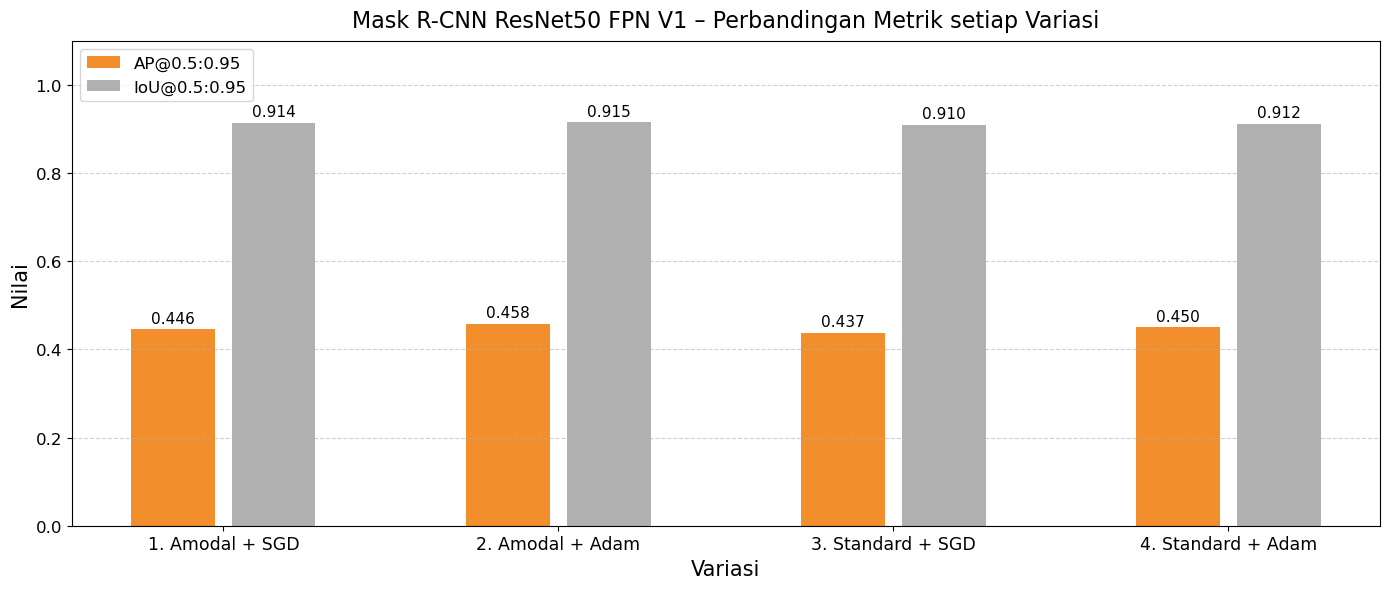
\includegraphics[width=1\textwidth]{figure/v1-version2d.png}
    \caption{Hasil Evaluasi \textit{Mask} R-CNN ResNet50 FPN V1}
    \label{fig:4.hasil_evaluasi_model_v1}
\end{figure}

Berdasarkan Tabel \ref{table:4.hasil_evaluasi_model_v1} dan Gambar \ref{fig:4.hasil_evaluasi_model_v1}, hasil evaluasi menggunakan metode \textit{K-Fold Cross Validation} menunjukkan bahwa variasi model \textit{Amodal} dengan \textit{optimizer} \textit{Adam} (variasi ke-2) menghasilkan performa rata-rata terbaik, dengan nilai \textit{AP50:95} sebesar 0{,}458 dan \textit{IoU50:95} sebesar 0{,}915. Secara spesifik, model terbaik diperoleh pada \textit{fold} pertama dengan capaian nilai \textit{AP50:95} mencapai 0{,}487 dengan \textit{IoU50:95} sebesar 0{,}915. Meskipun demikian, nilai \textit{IoU50:95} tertinggi justru diraih oleh variasi model \textit{Amodal} dengan \textit{optimizer} SGD (variasi ke-1), yaitu sebesar 0{,}919 pada \textit{fold} ke-4, meskipun dengan nilai \textit{AP50:95} yang sedikit lebih rendah, yaitu 0{,}449. \par

\subsection{Hasil Evaluasi \textit{Mask} R-CNN ResNet50 FPN V2}
Hasil evaluasi \textit{Model Pre-trained} \textit{Mask} R-CNN ResNet50 FPN V2 dengan variasi konfigurasi pelatihan dan dihitung metrik AP dan IoU ditampilkan pada Tabel \ref{table:4.hasil_evaluasi_model_v2}.

\begin{table}[H]
\centering
\caption{Hasil Evaluasi \textit{Mask} R-CNN ResNet50 FPN V2}
\label{table:4.hasil_evaluasi_model_v2}
% \footnotesize
\small
% \setlength{\tabcolsep}{6pt} % Menyesuaikan jarak antar kolom agar lebih ramping
\makebox[\textwidth][c]{
\begin{tabular}{|c|c|c|c|c|c|c|c|c|c|}
\hline
\multirow{2}{*}{\textbf{No}} & \multirow{2}{*}{\textbf{Model}} & \multirow{2}{*}{\textbf{Optim}} & \multirow{2}{*}{\textbf{Fold}} & \multicolumn{3}{c|}{\textbf{AP}} & \multicolumn{3}{c|}{\textbf{IoU}} \\
\cline{5-10}
& & & & \textbf{0.5} & \textbf{0.75} & \textbf{0.5:0.95} & \textbf{0.5} & \textbf{0.75} & \textbf{0.5:0.95} \\
\hline
\multirow{6}{*}{1} & \multirow{6}{*}{\textit{Amodal}} & \multirow{6}{*}{SGD} & 1 & 0{,}524 & 0{,}474 & 0{,}421 & 0{,}882 & 0{,}910 & 0{,}911 \\
\cline{4-10}
& & & 2 & 0{,}486 & 0{,}443 & 0{,}386 & 0{,}883 & 0{,}905 & 0{,}908 \\
\cline{4-10}
& & & 3 & 0{,}510 & 0{,}469 & 0{,}412 & 0{,}888 & 0{,}909 & 0{,}913 \\
\cline{4-10}
& & & 4 & 0{,}495 & 0{,}453 & 0{,}404 & 0{,}897 & 0{,}916 & 0{,}919 \\
\cline{4-10}
& & & 5 & 0{,}478 & 0{,}438 & 0{,}382 & 0{,}881 & 0{,}903 & 0{,}907 \\
\cline{4-10}
& & & Avg & 0{,}499 & 0{,}455 & 0{,}401 & 0{,}886 & 0{,}909 & 0{,}912 \\
\hline
\multirow{6}{*}{2} & \multirow{6}{*}{\textit{Amodal}} & \multirow{6}{*}{\textit{Adam}} & 1 & 0{,}545 & 0{,}509 & 0{,}447 & 0{,}893 & 0{,}912 & 0{,}915 \\
\cline{4-10}
& & & 2 & 0{,}524 & 0{,}481 & 0{,}424 & 0{,}892 & 0{,}910 & 0{,}913 \\
\cline{4-10}
& & & 3 & 0{,}503 & 0{,}456 & 0{,}405 & 0{,}888 & 0{,}909 & 0{,}912 \\
\cline{4-10}
& & & 4 & 0{,}504 & 0{,}466 & 0{,}408 & 0{,}888 & 0{,}908 & 0{,}911 \\
\cline{4-10}
& & & 5 & 0{,}510 & 0{,}473 & 0{,}417 & 0{,}889 & 0{,}908 & 0{,}912 \\
\cline{4-10}
& & & Avg & 0{,}517 & 0{,}477 & 0{,}420 & 0{,}890 & 0{,}909 & 0{,}913 \\
\hline
\multirow{6}{*}{3} & \multirow{6}{*}{\textit{Standard}} & \multirow{6}{*}{SGD} & 1 & 0{,}574 & 0{,}530 & \textbf{0{,}472} & 0{,}894 & 0{,}914 & 0{,}916 \\
\cline{4-10}
& & & 2 & 0{,}550 & 0{,}510 & 0{,}442 & 0{,}886 & 0{,}905 & 0{,}909 \\
\cline{4-10}
& & & 3 & 0{,}541 & 0{,}504 & 0{,}453 & 0{,}893 & 0{,}914 & 0{,}917 \\
\cline{4-10}
& & & 4 & 0{,}543 & 0{,}503 & 0{,}448 & 0{,}898 & 0{,}914 & 0{,}917 \\
\cline{4-10}
& & & 5 & 0{,}526 & 0{,}484 & 0{,}428 & 0{,}891 & 0{,}909 & 0{,}914 \\
\cline{4-10}
& & & \cellcolor{black!15}Avg & 0{,}547 & 0{,}506 & \cellcolor{black!15}\textbf{0{,}449} & 0{,}892 & 0{,}911 & \cellcolor{black!15}\textbf{0{,}915} \\
\hline
\multirow{6}{*}{4} & \multirow{6}{*}{\textit{Standard}} & \multirow{6}{*}{\textit{Adam}} & 1 & 0{,}568 & 0{,}525 & 0{,}463 & 0{,}891 & 0{,}912 & 0{,}914 \\
\cline{4-10}
& & & 2 & 0{,}550 & 0{,}511 & 0{,}444 & 0{,}886 & 0{,}906 & 0{,}909 \\
\cline{4-10}
& & & 3 & 0{,}534 & 0{,}490 & 0{,}437 & 0{,}892 & 0{,}910 & 0{,}914 \\
\cline{4-10}
& & & 4 & 0{,}542 & 0{,}507 & 0{,}454 & 0{,}900 & 0{,}918 & \textbf{0{,}921} \\
\cline{4-10}
& & & 5 & 0{,}550 & 0{,}505 & 0{,}443 & 0{,}892 & 0{,}911 & 0{,}915 \\
\cline{4-10}
& & & Avg & 0{,}547 & 0{,}506 & 0{,}448 & 0{,}892 & 0{,}912 & 0{,}914 \\
\hline
\end{tabular}
}
\end{table}

Visualisasi dari hasil evaluasi \textit{Mask} R-CNN ResNet50 FPN V2 ditampilkan pada Gambar \ref{fig:4.hasil_evaluasi_model_v2}.

\begin{figure}[H] % Kalau menggunakan H, posisi gambar akan tepat dibawah teks
    \centering
    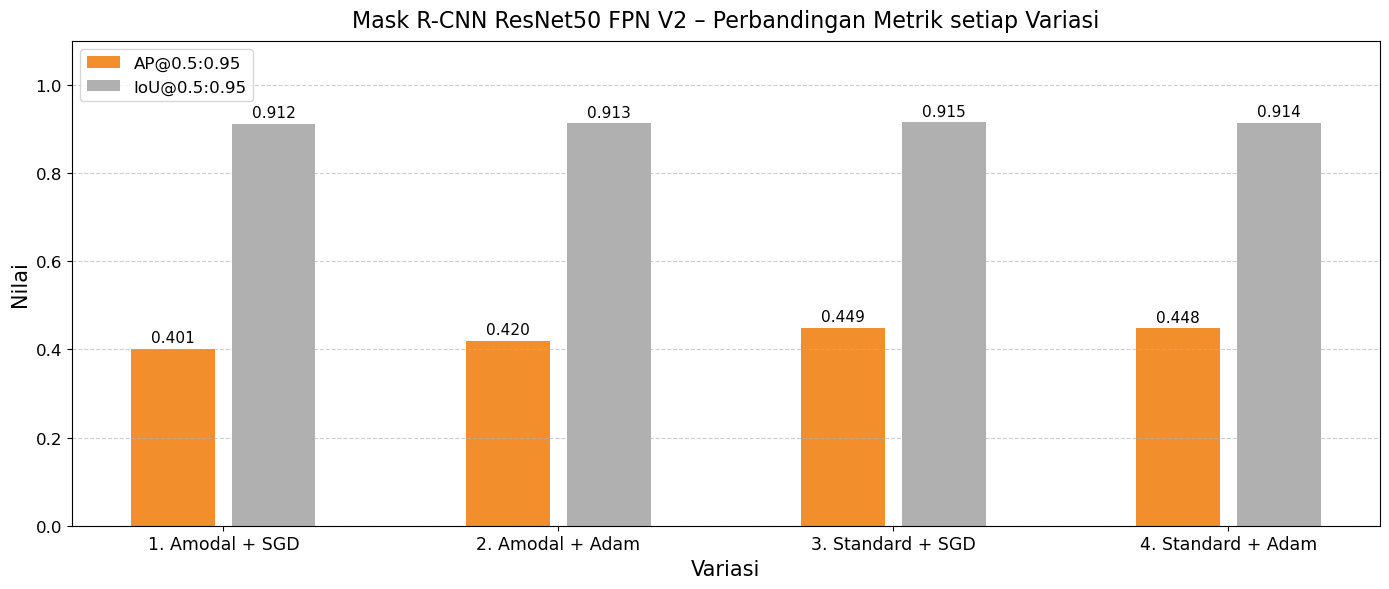
\includegraphics[width=1\textwidth]{figure/v2-version2d.png}
    \caption{Hasil Evaluasi \textit{Mask} R-CNN ResNet50 FPN V2}
    \label{fig:4.hasil_evaluasi_model_v2}
\end{figure}

Berdasarkan Tabel \ref{table:4.hasil_evaluasi_model_v2} dan Gambar \ref{fig:4.hasil_evaluasi_model_v2}, hasil evaluasi menggunakan metode \textit{K-Fold Cross Validation} menunjukkan bahwa variasi model \textit{Standard} dengan \textit{optimizer} SGD (variasi ke-3) menghasilkan performa rata-rata terbaik, dengan nilai \textit{AP50:95} sebesar 0{,}449 dan \textit{IoU50:95} sebesar 0{,}915. Secara spesifik, model terbaik diperoleh pada \textit{fold} pertama dengan capaian nilai \textit{AP50:95} mencapai 0{,}472 dengan \textit{IoU50:95} sebesar 0{,}916. Meskipun demikian, nilai \textit{IoU50:95} tertinggi justru dicapai oleh variasi model \textit{Standard} dengan \textit{optimizer} \textit{Adam} (variasi ke-4), yaitu sebesar 0{,}921 pada \textit{fold} ke-4, meskipun dengan nilai \textit{AP50:95} yang sedikit lebih rendah, yaitu 0{,}454. \par

\section{Perbandingan Evaluasi Model} \label{IV.Perbandingan_Evaluasi_Model}
Hasil pertimbangan dari kedua model \textit{pre-trained} berdasarkan variasi konfigurasi pelatihan dengan performa terbaik berdasarkan rata-rata metrik \textit{AP50:95} dari hasil metode \textit{K-Fold Cross Validation} yang ditampilkan pada Tabel \ref{table:4.perbandingan_evaluasi_model}.

\begin{table}[H]
\centering
\caption{Hasil Perbandingan Evaluasi Model Terbaik}
\label{table:4.perbandingan_evaluasi_model}
\small
\makebox[\textwidth][c]{
\begin{tabular}{|c|c|c|c|c|}
\hline
\multirow{2}{*}{\textbf{Model \textit{Pre-trained}}} & \multirow{2}{*}{\textbf{Model}} & \multirow{2}{*}{\textbf{Optimizer}} & \textbf{AP} & \textbf{IoU} \\
\cline{4-5}
& & & \textbf{0.5:0.95} & \textbf{0.5:0.95} \\
\hline
\textbf{\textit{Mask} R-CNN ResNet50 FPN V1} & \textbf{\textit{Amodal}} & \textbf{\textit{Adam}} & \textbf{0{,}458} & \textbf{0{,}915} \\
\hline
\textit{Mask} R-CNN ResNet50 FPN V1 & \textit{Standard} & SGD & 0{,}437 & 0{,}910 \\
\hline
\textit{Mask} R-CNN ResNet50 FPN V2 & \textit{Amodal} & \textit{Adam} & 0{,}420 & 0{,}913 \\
\hline
\textbf{\textit{Mask} R-CNN ResNet50 FPN V2} & \textbf{\textit{Standard}} & \textbf{SGD} & \textbf{0{,}449} & \textbf{0{,}915} \\
\hline
\end{tabular}
}
\end{table}

Berdasarkan Tabel \ref{table:4.perbandingan_evaluasi_model}, dapat dilihat bahwa hasil perbandingan dua model terbaik didapatkan bahwa model \textit{pre-trained} \textit{Mask} R-CNN ResNet50 FPN V1 dengan variasi model \textit{Amodal} dan \textit{optimizer} \textit{Adam} menunjukkan performa terbaik dengan nilai \textit{AP50:95} sebesar 0{,}458 dan \textit{IoU50:95} sebesar 0{,}915. Model \textit{pre-trained} \textit{Mask} R-CNN ResNet50 FPN V2 dengan variasi model \textit{Standard} dan \textit{optimizer} SGD menunjukkan performa yang sedikit lebih rendah dengan nilai \textit{AP50:95} sebesar 0{,}449 dan \textit{IoU50:95} sebesar 0{,}915. \par

Performa unggul model dengan \textit{optimizer} \textit{Adam} dapat dilihat secara konsisten pada hasil evaluasi. Berdasarkan Tabel \ref{table:4.hasil_evaluasi_model_v1} untuk model V1 dan Tabel \ref{table:4.hasil_evaluasi_model_v2} untuk model V2, penggunaan \textit{optimizer} \textit{Adam} menghasilkan nilai \textit{AP50:95} yang lebih tinggi dibandingkan dengan \textit{optimizer} SGD. Keunggulan ini disebabkan oleh mekanisme \textit{adaptive learning rate} yang dimiliki \textit{Adam}, yang mampu mempercepat dan menstabilkan proses konvergensi, terutama pada objek dengan bentuk kompleks seperti citra mikroskop mineral kasiterit \cite{optimizer}. Sifat adaptif ini menjadikan \textit{Adam} lebih efektif untuk pendekatan \textit{amodal} yang memerlukan kemampuan prediksi lebih kompleks. Sementara itu, \textit{optimizer} SGD tetap menunjukkan stabilitas yang baik dalam proses pembelajaran pada pendekatan segmentasi standar, meskipun nilai \textit{AP50:95} yang dihasilkan sedikit lebih rendah, dengan selisih 0{,}009 dibandingkan model \textit{pre-trained Mask R-CNN ResNet50 FPN V2} dengan variasi model \textit{Standard} dan \textit{optimizer} SGD. Berdasarkan hasil evaluasi tersebut, dapat disimpulkan bahwa konfigurasi terbaik dalam penelitian ini adalah model \textit{pre-trained Mask R-CNN ResNet50 FPN V1} dengan variasi model \textit{Amodal} dan \textit{optimizer} \textit{Adam}. \par

\begin{table}[H]
\centering
\caption{Hasil Perbandingan Penerapan Amodal}
\label{table:4.perbandingan_penerapan_amodal}
\small
\makebox[\textwidth][c]{
\begin{tabular}{|c|c|c|c|c|c|c|}
\hline
\multirow{2}{*}{\textbf{Model \textit{Pre-trained}}} & \multirow{2}{*}{\textbf{Model}} & \multirow{2}{*}{\textbf{Optimizer}} & \multirow{2}{*}{\textbf{Parameter}} & \textbf{AP} & \textbf{IoU} & \multirow{2}{*}{\textbf{Waktu \textit{Train}}} \\
\cline{5-6}
& & & & \textbf{0.5:0.95} & \textbf{0.5:0.95} & \\
\hline
\textbf{\textit{Mask} R-CNN V1} & \textbf{\textit{Amodal}} & \textbf{\textit{Adam}} & \textbf{46,650,909} & \textbf{0{,}458} & \textbf{0{,}915} & \textbf{4.46 jam} \\
\hline
\textit{Mask} R-CNN V1 & \textit{Standard} & SGD & 43,699,995  & 0{,}437 & 0{,}910 & 4.09 jam \\
\hline
\textit{Mask} R-CNN V2 & \textit{Amodal} & \textit{Adam} & 48,605,981 & 0{,}420 & 0{,}913 & 4.14 jam \\
\hline
\textbf{\textit{Mask} R-CNN V2} & \textbf{\textit{Standard}} & \textbf{SGD} & \textbf{45,655,067} & \textbf{0{,}449} & \textbf{0{,}915} & \textbf{3.69 jam} \\
\hline
\end{tabular}
}
\end{table}

Berdasarkan Tabel \ref{table:4.perbandingan_penerapan_amodal}, penerapan teknik \textit{Amodal Instance Segmentation} menunjukkan pengaruh yang berbeda pada masing-masing model \textit{pre-trained} \textit{Mask} R-CNN yang diuji. Pada model \textit{pre-trained} \textit{Mask} R-CNN ResNet50 FPN V1 dengan \textit{optimizer} \textit{Adam}, penambahan teknik \textit{amodal} yang meningkatkan jumlah parameter sebesar 2{,}950{,}914 (sekitar 6{,}75\%) menghasilkan peningkatan performa, ditunjukkan oleh kenaikan nilai \textit{AP50:95} sebesar 0{,}021 (dari 0{,}437 menjadi 0{,}458) serta peningkatan \textit{IoU50:95} sebesar 0{,}005 (dari 0{,}910 menjadi 0{,}915). Peningkatan ini disertai dengan penambahan waktu pelatihan sebesar 0{,}37 jam, yang masih berada dalam batas komputasi yang dapat diterima untuk skenario segmentasi objek dengan tingkat oklusi tinggi.

Sebaliknya, pada model \textit{pre-trained} \textit{Mask} R-CNN ResNet50 FPN V2 dengan \textit{optimizer} SGD, penerapan teknik \textit{amodal}  yang meningkatkan jumlah parameter sebesar 2{,}950{,}914 (sekitar 6{,}46\%) tidak memberikan peningkatan performa. Nilai \textit{AP50:95} justru mengalami penurunan sebesar 0{,}029 (dari 0{,}449 menjadi 0{,}420), sementara nilai \textit{IoU50:95} menurun sebesar 0{,}002 (dari 0{,}915 menjadi 0{,}913), meskipun waktu pelatihan hanya bertambah 0{,}45 jam. Hasil ini menunjukkan bahwa penambahan kompleksitas model melalui pendekatan \textit{amodal} tidak selalu berbanding lurus dengan peningkatan kinerja, serta mengindikasikan bahwa efektivitas penerapan teknik \textit{Amodal Instance Segmentation} sangat bergantung pada kesesuaian dengan model \textit{pre-trained} dan pemilihan \textit{optimizer} yang digunakan.

\begin{table}[H]
\centering
\caption{Hasil Perbandingan Evaluasi Model Terbaik per Parameter}
\label{table:4.perbandingan_parameter_model}
\small
\makebox[\textwidth][c]{
\begin{tabular}{|c|c|c|c|c|c|c|}
\hline
\multirow{2}{*}{\parbox{2.5cm}{\centering\textbf{Model \textit{Pre-trained}}}} & \multirow{2}{*}{\textbf{Model}} & \multirow{2}{*}{\textbf{Optim}} & \multirow{2}{*}{\textbf{Parameter}} & \multirow{2}{*}{\parbox{1.1cm}{\centering\textbf{Param Ratio}}} & \multicolumn{2}{c|}{\textbf{Perbandingan (Metrik/Param)}} \\
\cline{6-7}
& & & & & \parbox{1.85cm}{\centering\textbf{AP/Param}} & \textbf{IoU/Param} \\
\hline
\textit{Mask} R-CNN V1 & \textit{Amodal} & \textit{Adam} & 46,650,909 & 1{,}067$\times$ & 9{,}814e-9 & 1{,}962e-8 \\
\hline
\textbf{\textit{Mask} R-CNN V1} & \textbf{\textit{Standard}} & \textbf{SGD} & \textbf{43,699,995} & \textbf{1{,}000$\times$} & \textbf{9{,}999e-9} & \textbf{2{,}082e-8} \\
\hline
\textit{Mask} R-CNN V2 & \textit{Amodal} & \textit{Adam} & 48,605,981 & 1{,}113$\times$ & 8{,}644e-9 & 1{,}878e-8 \\
\hline
\textbf{\textit{Mask} R-CNN V2} & \textbf{\textit{Standard}} & \textbf{SGD} & \textbf{45,655,067} & \textbf{1{,}045$\times$} & \textbf{9{,}835e-9} & \textbf{2{,}004e-8} \\
\hline
\end{tabular}
}
\end{table}

Berdasarkan Tabel \ref{table:4.perbandingan_parameter_model}, evaluasi efisiensi parameter menunjukkan perbedaan kemampuan tiap model dalam memanfaatkan kompleksitas model terhadap kinerja yang dihasilkan. Model \textit{Mask} R-CNN ResNet50 FPN V1 \textit{Standard} dengan \textit{optimizer} SGD digunakan sebagai \textit{baseline} (\textit{Param Ratio} 1{,}000$\times$) dengan total 43.699.995 parameter dan menunjukkan efisiensi parameter tertinggi, ditunjukkan oleh rasio \textit{AP/Param} sebesar 9{,}999e-9 dan \textit{IoU/Param} sebesar 2{,}082e-8. Penerapan teknik \textit{amodal} pada model \textit{Mask} R-CNN V1 meningkatkan jumlah parameter menjadi 46.650.909 (\textit{Param Ratio} 1{,}067$\times$), namun tidak diikuti oleh peningkatan efisiensi, karena nilai \textit{AP/Param} dan \textit{IoU/Param} justru lebih rendah dibandingkan versi \textit{Standard}. \par

Hal yang sama juga terlihat pada model \textit{Mask} R-CNN ResNet50 FPN V2. Model \textit{Standard} dengan \textit{optimizer} SGD (\textit{Param Ratio} 1{,}045$\times$) menunjukkan rasio \textit{AP/Param} dan \textit{IoU/Param} yang lebih seimbang dibandingkan model V2 \textit{Amodal} (\textit{Param Ratio} 1{,}113$\times$). Meskipun model V1 \textit{Standard} \textit{optimizer} dengan SGD memiliki efisiensi parameter tertinggi, model V2 \textit{Standard} \textit{optimizer} dengan SGD merepresentasikan keseimbangan yang lebih baik antara kompleksitas model, efisiensi parameter, dan performa deteksi, sehingga lebih sesuai untuk penerapan praktis pada segmentasi mineral kasiterit. Secara keseluruhan, hasil ini menunjukkan bahwa peningkatan jumlah parameter melalui pendekatan \textit{amodal} tidak selalu berbanding lurus dengan peningkatan efisiensi model. \par


\section{Pengujian Model} \label{IV.Pengujian_Model}
Pengujian model akan di lakukan menggunakan ke dua model terbaik yang telah di dapatkan dari hasil evaluasi pada Bagian \ref{IV.Perbandingan_Evaluasi_Model}, yaitu model \textit{pre-trained} \textit{Mask} R-CNN ResNet50 FPN V1 dengan variasi model \textit{Amodal} dan \textit{optimizer} \textit{Adam} (V1 \textit{Am}) serta model \textit{pre-trained} \textit{Mask} R-CNN ResNet50 FPN V2 dengan variasi model \textit{Standard} dan \textit{optimizer} SGD (V2 \textit{Std}). Pengujian dilakukan pada 6 citra uji yang berbeda dari dataset pelatihan. Hasil pengujian ditampilkan pada Tabel \ref{table:4.Pengujian1}. Evaluasi kinerja prediksi dilakukan berdasarkan beberapa kategori evaluasi prediksi yang ditentukan dengan mempertimbangkan nilai \textit{Intersection over Union} (IoU) antara prediksi dan \textit{ground truth}, skor kepercayaan (\textit{confidence score}), serta kesesuaian label objek. Berdasarkan kriteria tersebut, hasil prediksi dikelompokkan ke dalam lima kategori, yaitu \textit{Correct}, \textit{Low Confidence}, \textit{Wrong Location}, \textit{False Positive}, dan \textit{False Negative}. 

Pada pengujian ini, evaluasi hasil prediksi model dilakukan dengan mengelompokkan setiap prediksi ke dalam beberapa kategori evaluasi prediksi berdasarkan nilai \textit{Intersection over Union} (IoU), skor kepercayaan (\textit{confidence score}), serta kesesuaian label prediksi terhadap \textit{ground truth}. Nilai ambang batas (\textit{threshold}) dan ambang batas IoU (\textit{IoU threshold}) ditetapkan sebesar 0,5 \cite{threshold_pengujian}, sedangkan ambang batas kepercayaan (\textit{confidence threshold}) ditetapkan sebesar 0,7. prediksi dikategorikan sebagai \textit{Correct} apabila memiliki nilai IoU $\geq 0,5$, skor kepercayaan $\geq 0,7$, dan label prediksi sesuai dengan \textit{ground truth}. Kategori \textit{Low Confidence} diberikan pada prediksi dengan IoU $\geq 0,5$ dan label yang benar, namun skor kepercayaan $<$ 0,7. Prediksi dengan label yang sesuai tetapi memiliki nilai IoU $<$ 0,5 diklasifikasikan sebagai \textit{Wrong Location}. Selanjutnya, \textit{False Positive} merupakan prediksi yang tidak memiliki pasangan \textit{ground truth} yang sesuai atau memiliki label yang tidak cocok, sedangkan \textit{False Negative} merupakan objek pada \textit{ground truth} yang tidak berhasil terprediksi oleh model.

% Atur margin untuk landscape - bisa disesuaikan nilai left dan right
\newgeometry{top=2cm, bottom=1.75cm, left=2cm, right=2cm}

\begin{landscape}
% \thispagestyle{landscape} % Untuk page number yang benar di landscape
\renewcommand{\arraystretch}{1.2} % Mengatur jarak antar baris tabel
\centering 
\begin{longtable}{|c|c|c|c|c|c|c|c|c|c|c|c|c|}
    \caption{Hasil Pengujian Model}
    \label{table:4.Pengujian1}\\
    \hline
    \multirow{2}{*}{\parbox{0.375cm}{\centering\textbf{No}}} & 
    \multirow{2}{*}{\parbox{4.0cm}{\centering\textbf{Citra}}} & 
    \multirow{2}{*}{\parbox{0.75cm}{\centering\textbf{GT\\Total}}} & 
    \multicolumn{8}{c|}{\textbf{Prediksi}} &
    \multirow{2}{*}{\parbox{1.2cm}{\centering\textbf{Hitung\\Manual}}} &
    \multirow{2}{*}{\parbox{1cm}{\centering\textbf{Model}}} \\
    \cline{4-11}
    & & &
    \parbox{0.75cm}{\centering\textbf{Total}} &
    \parbox{1.1cm}{\centering\textbf{Correct}} &
    \parbox{0.7cm}{\centering\textbf{\shortstack{Low\\[-0.2em]Conf}}} &
    \parbox{0.95cm}{\centering\textbf{\shortstack{Wrong\\[-0.35em]Loc}}} &
    \parbox{0.7cm}{\centering\textbf{\shortstack{False\\[-0.2em]Pos}}} &
    \parbox{0.7cm}{\centering\textbf{\shortstack{False\\[-0.2em]Neg}}} &
    \parbox{0.95cm}{\centering\textbf{\shortstack{AP\\[-0.2em]50:95}}} &
    \parbox{0.95cm}{\centering\textbf{\shortstack{IoU\\[-0.2em]50:95}}} &
    & \\

    \hline
    \endfirsthead
    
    \hline
    \multirow{2}{*}{\parbox{0.375cm}{\centering\textbf{No}}} & 
    \multirow{2}{*}{\parbox{4.0cm}{\centering\textbf{Citra}}} & 
    \multirow{2}{*}{\parbox{0.75cm}{\centering\textbf{GT\\Total}}} & 
    \multicolumn{8}{c|}{\textbf{Prediksi}} &
    \multirow{2}{*}{\parbox{1.2cm}{\centering\textbf{Hitung\\Manual}}} &
    \multirow{2}{*}{\parbox{1cm}{\centering\textbf{Model}}} \\
    \cline{4-11}
    & & &
    \parbox{0.75cm}{\centering\textbf{Total}} &
    \parbox{1.1cm}{\centering\textbf{Correct}} &
    \parbox{0.7cm}{\centering\textbf{\shortstack{Low\\[-0.2em]Conf}}} &
    \parbox{0.95cm}{\centering\textbf{\shortstack{Wrong\\[-0.35em]Loc}}} &
    \parbox{0.7cm}{\centering\textbf{\shortstack{False\\[-0.2em]Pos}}} &
    \parbox{0.7cm}{\centering\textbf{\shortstack{False\\[-0.2em]Neg}}} &
    \parbox{0.95cm}{\centering\textbf{\shortstack{AP\\[-0.2em]50:95}}} &
    \parbox{0.95cm}{\centering\textbf{\shortstack{IoU\\[-0.2em]50:95}}} &
    & \\
    \hline
    \endhead
    
    \hline
    \endfoot
    
    \hline
    \endlastfoot
    
    % ===== Data ke-1 =====
    \multirow{2}{*}{1} &
    \multirow{2}{*}{%
    \parbox[c][1.5cm][c]{4cm}{%
    \centering
    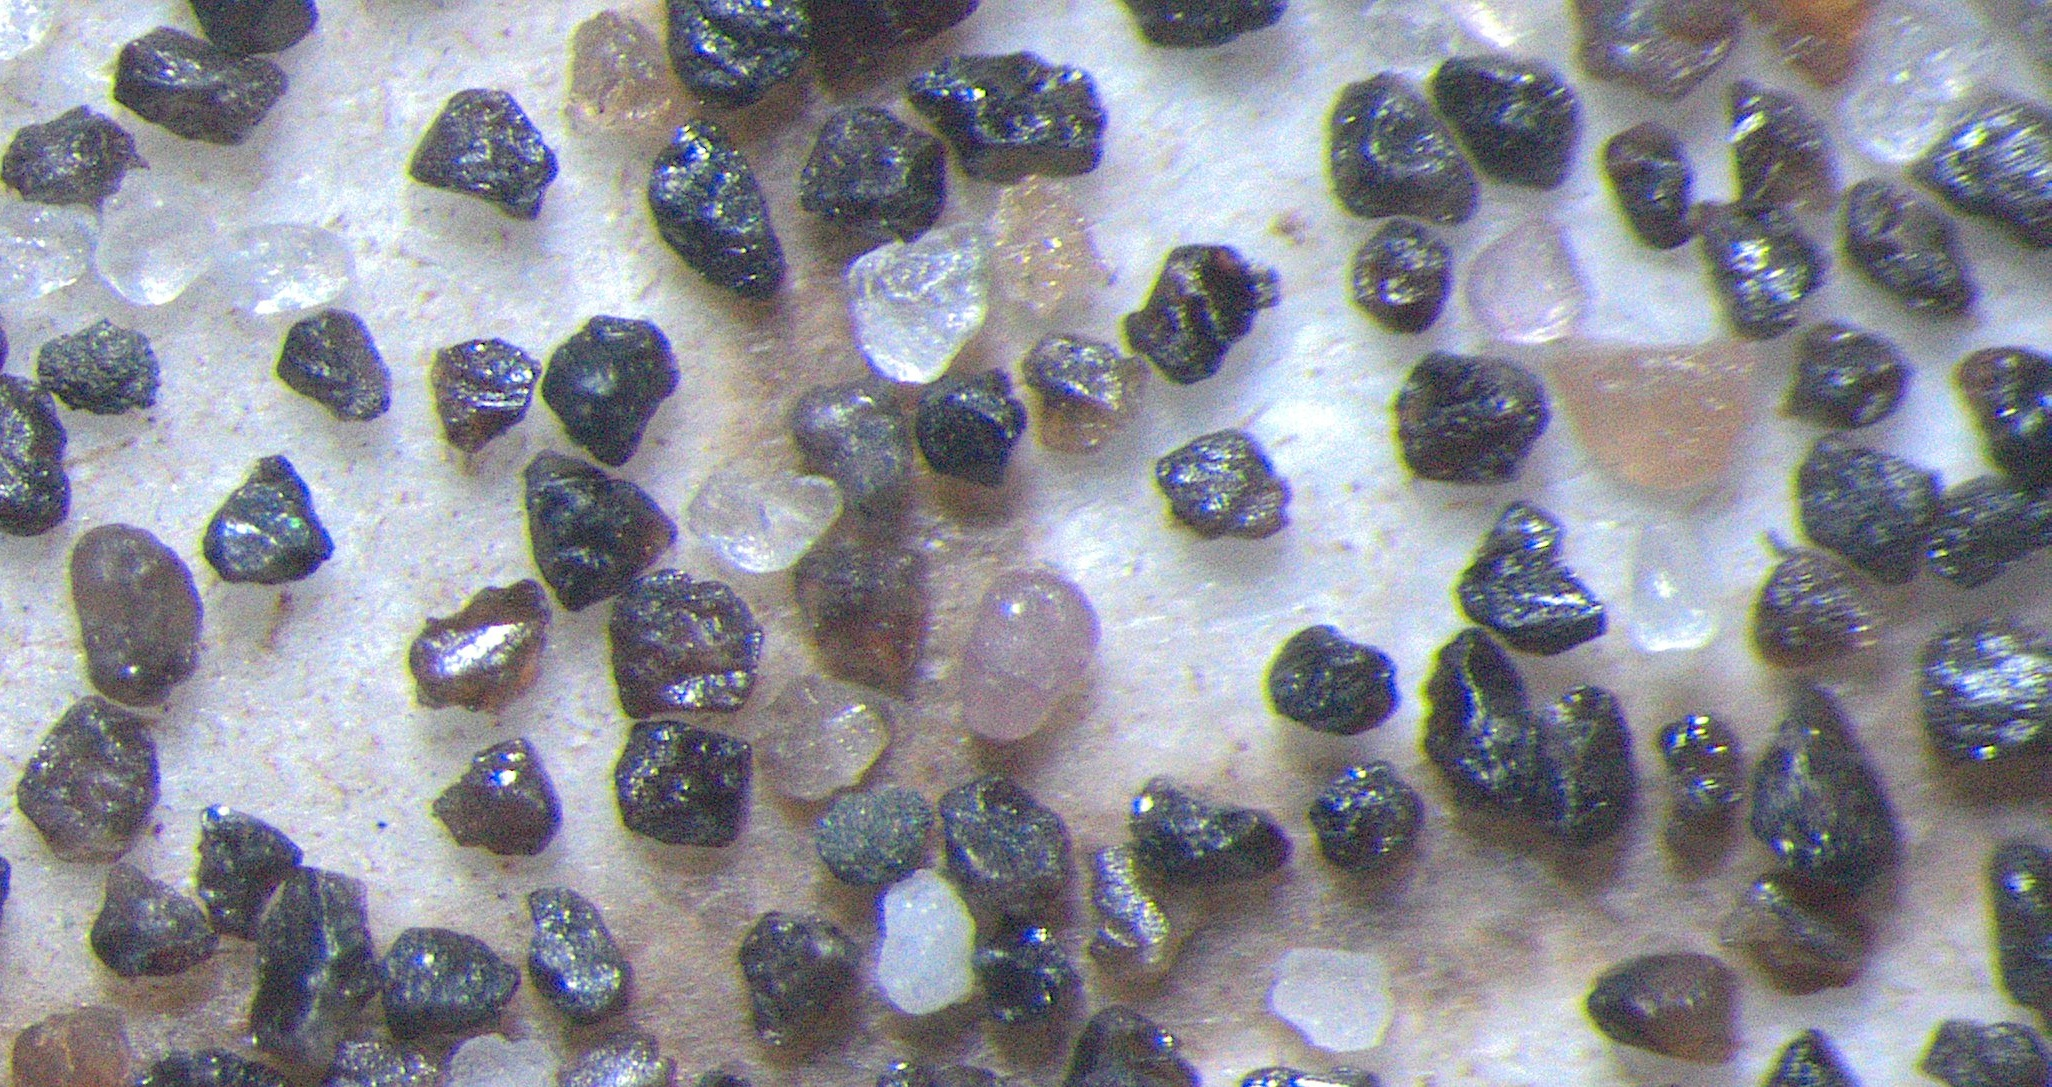
\includegraphics[width=4.05cm,height=4cm,keepaspectratio]{figure/pengujian/1/0384-16_100C_tile1.jpg}}} &
    \multirow{2}{*}{18} &

    34\rule{0pt}{3.0em} & 11 & 0 & 1 & 22 & 6 & 0{,}567 & 0{,}938 & 11 &
    V1 \textit{(Am)} \\

    \cline{4-13}

    & & &   % ← WAJIB: kosongkan No | Citra | GT Total
    36\rule{0pt}{3.0em} & 10 & 1 & 1 & 24 & 6 & 0{,}552 & 0{,}916 & 11 &
    V2 \textit{(Std)} \\

    \hline
    
    % ===== Data ke-2 =====
    \multirow{2}{*}{2} &
    \multirow{2}{*}{%
    \parbox[c][1.5cm][c]{4cm}{%
    \centering
    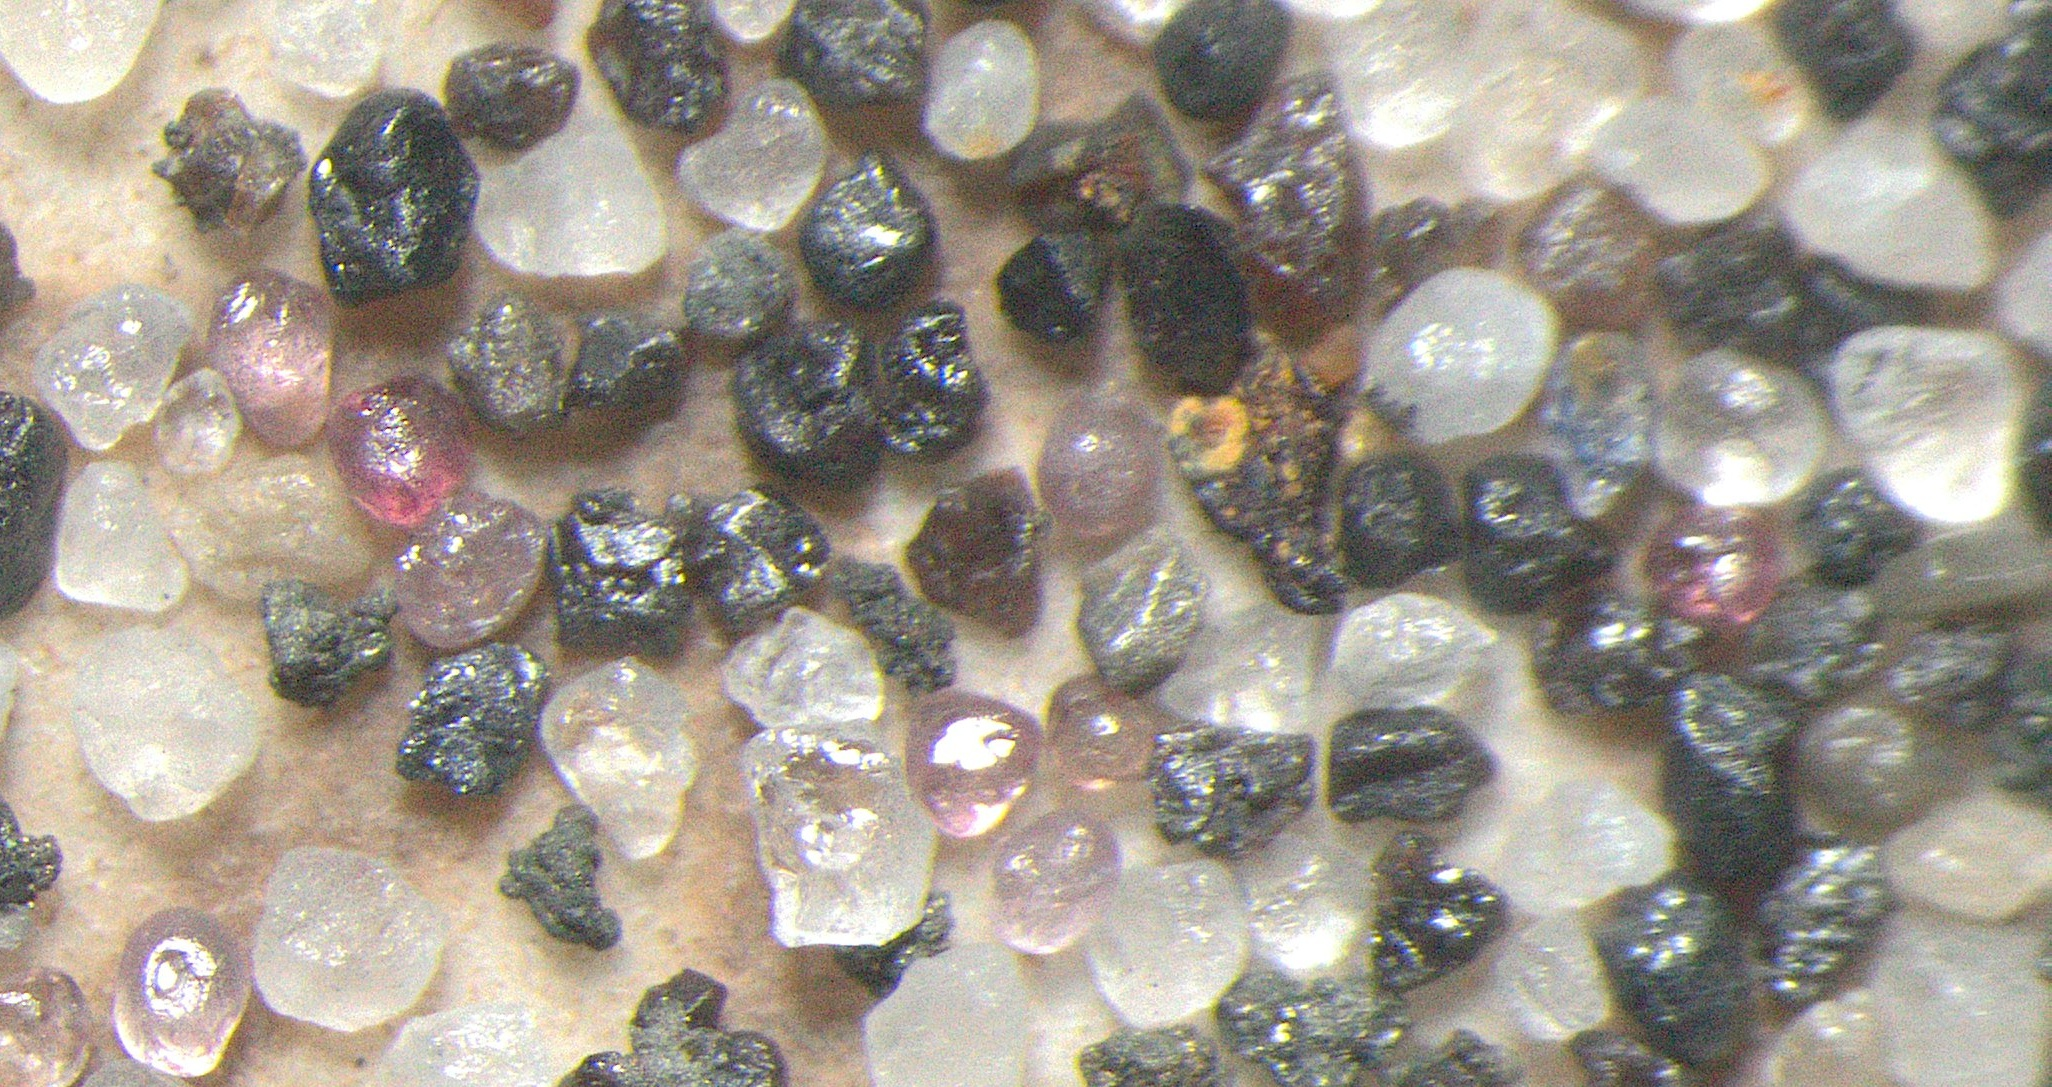
\includegraphics[width=4.05cm,height=4cm,keepaspectratio]{figure/pengujian/2/0384-16_48C_tile1.jpg}}} &
    \multirow{2}{*}{8} &

    16\rule{0pt}{3.0em} & 5 & 1 & 0 & 10 & 2 & 0{,}675 & 0{,}940 & 6 &
    V1 \textit{(Am)} \\

    \cline{4-13}

    & & &   % ← WAJIB: kosongkan No | Citra | GT Total
    28\rule{0pt}{3.0em} & 7 & 1 & 0 & 20 & 0 & 0{,}838 & 0{,}920 & 8 &
    V2 \textit{(Std)} \\

    \hline

    % ===== Data ke-3 =====
    \multirow{2}{*}{3} &
    \multirow{2}{*}{%
    \parbox[c][1.5cm][c]{4cm}{%
    \centering
    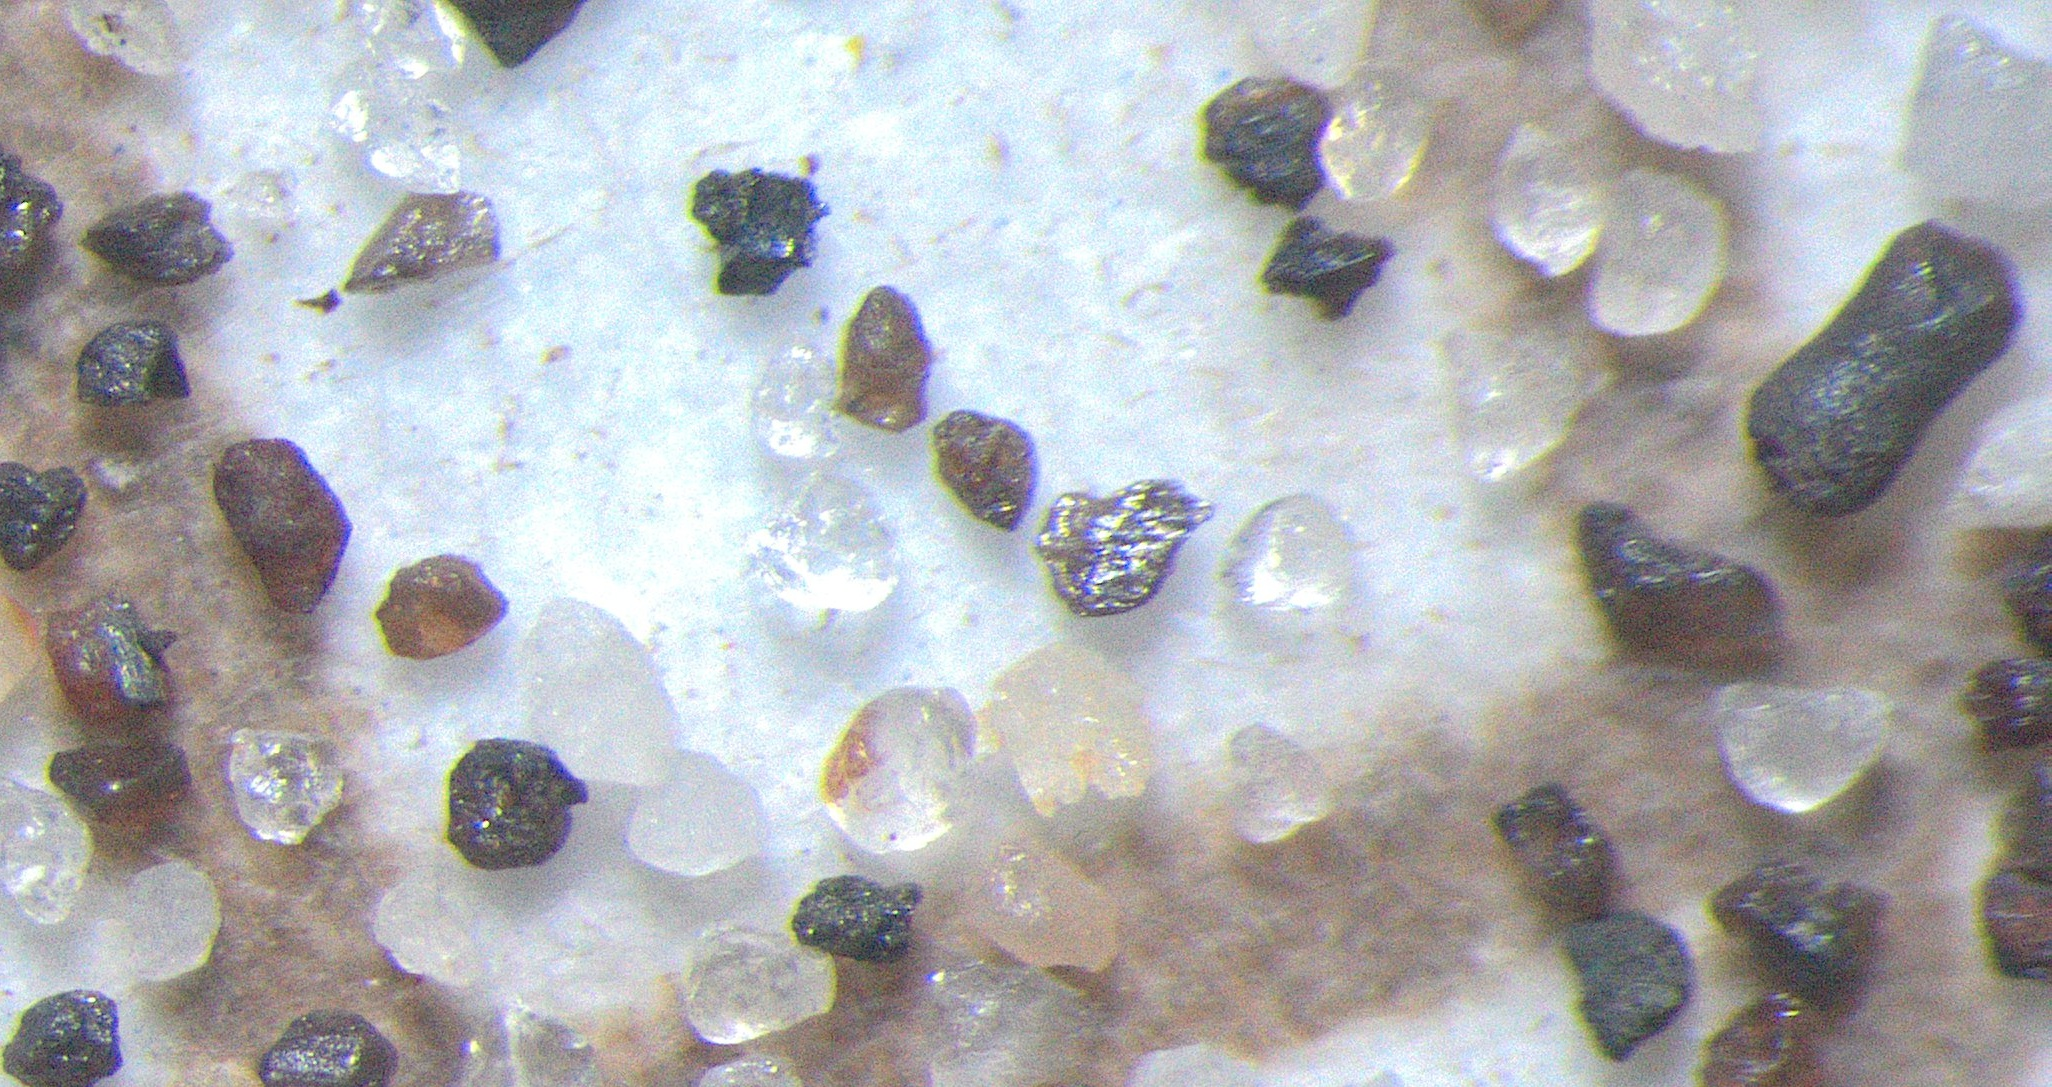
\includegraphics[width=4.05cm,height=4cm,keepaspectratio]{figure/pengujian/3/1347-20_100H_tile1.jpg}}} &
    \multirow{2}{*}{10} &

    21\rule{0pt}{3.0em} & 7 & 2 & 0 & 12 & 1 & 0{,}830 & 0{,}936 & 9 &
    V1 \textit{(Am)} \\

    \cline{4-13}

    & & &   % ← WAJIB: kosongkan No | Citra | GT Total
    19\rule{0pt}{3.0em} & 6 & 3 & 0 & 10 & 1 & 0{,}820 & 0{,}931 & 9 &
    V2 \textit{(Std)} \\

    \hline
\end{longtable}
\end{landscape}
\restoregeometry

    
\newgeometry{top=2cm, bottom=1.75cm, left=2cm, right=2cm}

\begin{landscape}
% \thispagestyle{landscape} % Untuk page number yang benar di landscape
\renewcommand{\arraystretch}{1.2} % Mengatur jarak antar baris tabel
\centering 
\begin{longtable}{|c|c|c|c|c|c|c|c|c|c|c|c|c|}
    % \caption{Hasil Pengujian Model}
    % \label{table:4.Pengujian4}\\
    \hline
    \multirow{2}{*}{\parbox{0.375cm}{\centering\textbf{No}}} & 
    \multirow{2}{*}{\parbox{4.0cm}{\centering\textbf{Citra}}} & 
    \multirow{2}{*}{\parbox{0.75cm}{\centering\textbf{GT\\Total}}} & 
    \multicolumn{8}{c|}{\textbf{Prediksi}} &
    \multirow{2}{*}{\parbox{1.2cm}{\centering\textbf{Hitung\\Manual}}} &
    \multirow{2}{*}{\parbox{0.85cm}{\centering\textbf{Model}}} \\
    \cline{4-11}
    & & &
    \parbox{0.75cm}{\centering\textbf{Total}} &
    \parbox{1.1cm}{\centering\textbf{Correct}} &
    \parbox{0.7cm}{\centering\textbf{\shortstack{Low\\[-0.2em]Conf}}} &
    \parbox{0.95cm}{\centering\textbf{\shortstack{Wrong\\[-0.35em]Loc}}} &
    \parbox{0.7cm}{\centering\textbf{\shortstack{False\\[-0.2em]Pos}}} &
    \parbox{0.7cm}{\centering\textbf{\shortstack{False\\[-0.2em]Neg}}} &
    \parbox{0.95cm}{\centering\textbf{\shortstack{AP\\[-0.2em]50:95}}} &
    \parbox{0.95cm}{\centering\textbf{\shortstack{IoU\\[-0.2em]50:95}}} &
    & \\

    \hline
    \endfirsthead
    
    \hline
    \multirow{2}{*}{\parbox{0.375cm}{\centering\textbf{No}}} & 
    \multirow{2}{*}{\parbox{4.0cm}{\centering\textbf{Citra}}} & 
    \multirow{2}{*}{\parbox{0.75cm}{\centering\textbf{GT\\Total}}} & 
    \multicolumn{8}{c|}{\textbf{Prediksi}} &
    \multirow{2}{*}{\parbox{1.2cm}{\centering\textbf{Hitung\\Manual}}} &
    \multirow{2}{*}{\parbox{0.85cm}{\centering\textbf{Model}}} \\
    \cline{4-11}
    & & &
    \parbox{0.75cm}{\centering\textbf{Total}} &
    \parbox{1.1cm}{\centering\textbf{Correct}} &
    \parbox{0.7cm}{\centering\textbf{\shortstack{Low\\[-0.2em]Conf}}} &
    \parbox{0.95cm}{\centering\textbf{\shortstack{Wrong\\[-0.35em]Loc}}} &
    \parbox{0.7cm}{\centering\textbf{\shortstack{False\\[-0.2em]Pos}}} &
    \parbox{0.7cm}{\centering\textbf{\shortstack{False\\[-0.2em]Neg}}} &
    \parbox{0.95cm}{\centering\textbf{\shortstack{AP\\[-0.2em]50:95}}} &
    \parbox{0.95cm}{\centering\textbf{\shortstack{IoU\\[-0.2em]50:95}}} &
    & \\
    \hline
    \endhead
    
    \hline
    \endfoot
    
    \hline
    \endlastfoot

    % ===== Data ke-4 =====
    \multirow{2}{*}{4} &
    \multirow{2}{*}{%
    \parbox[c][1.5cm][c]{4cm}{%
    \centering
    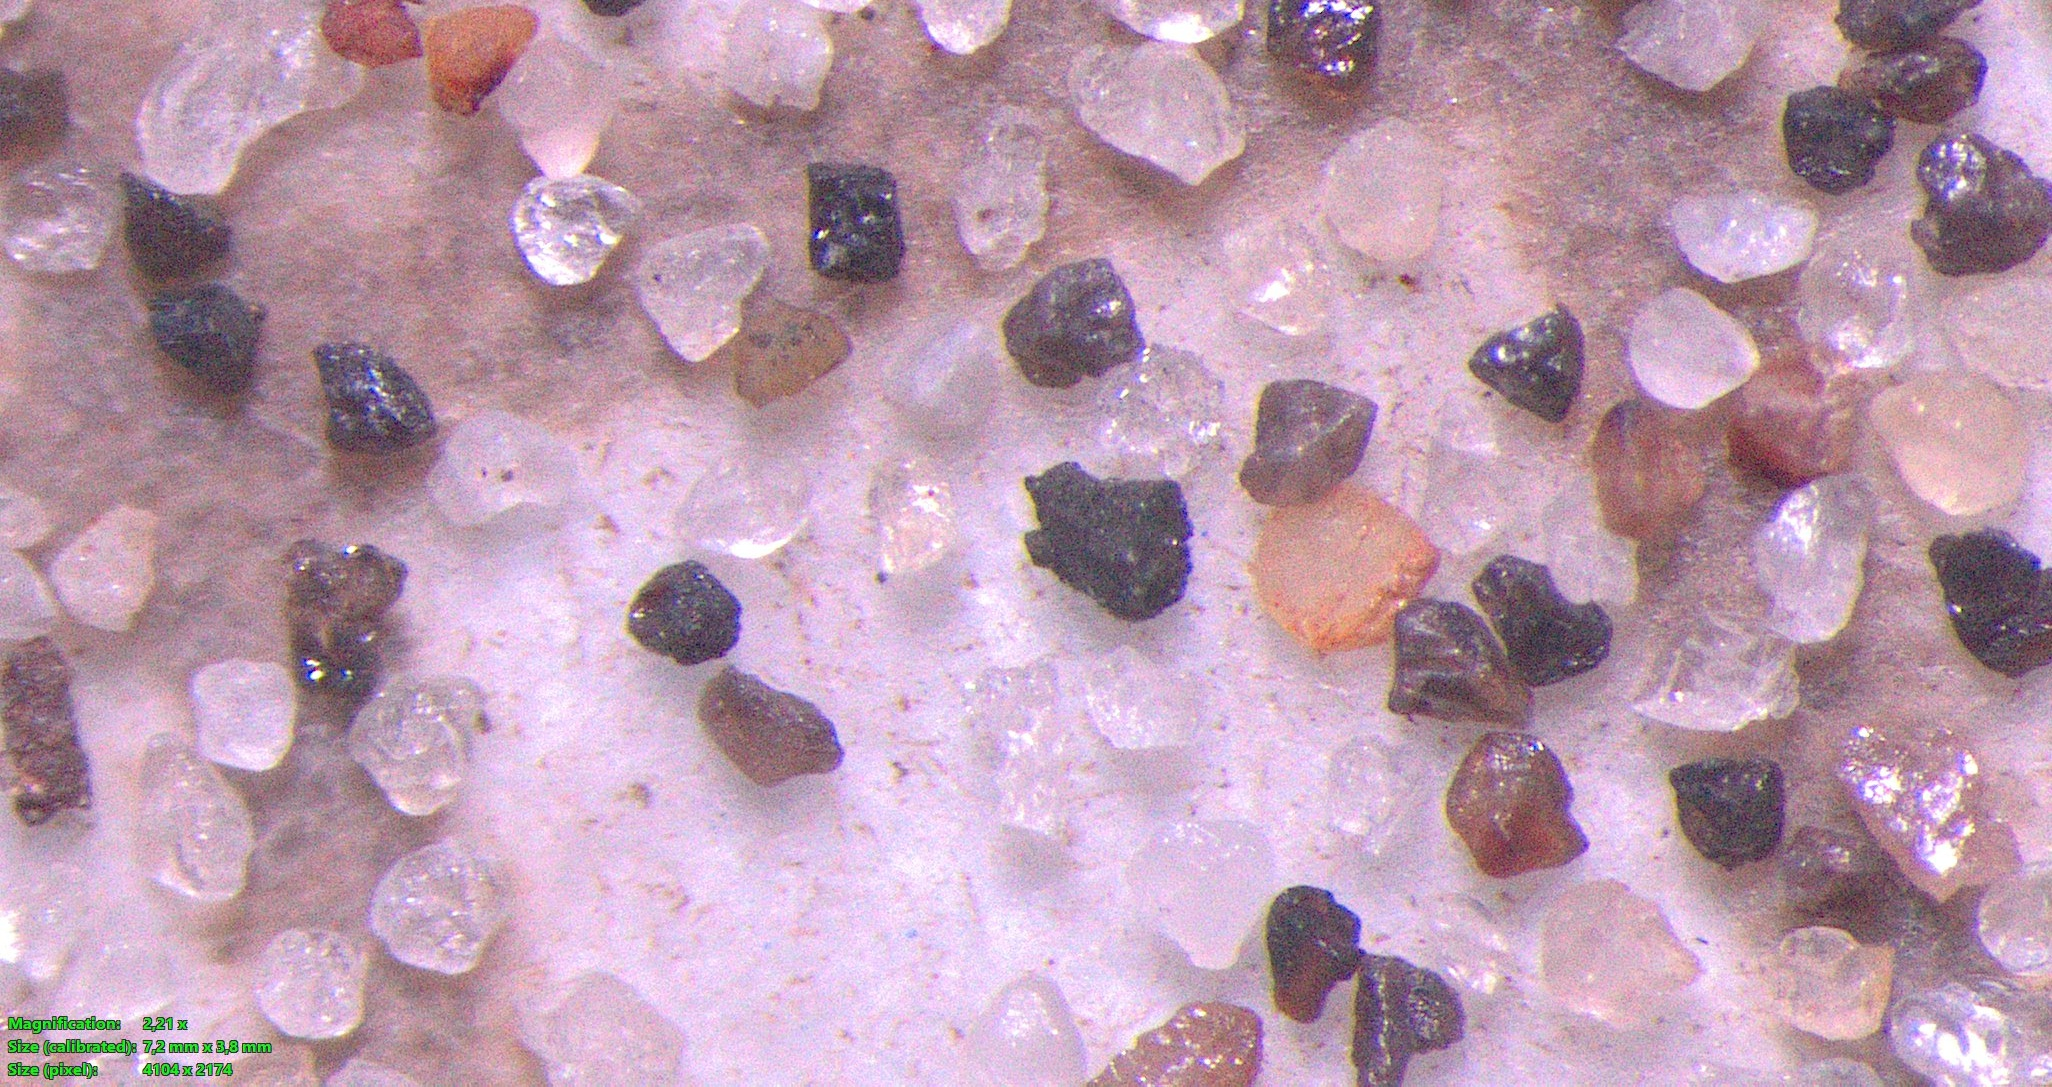
\includegraphics[width=4.05cm,height=4cm,keepaspectratio]{figure/pengujian/4/1347-17_100G_tile2.jpg}}} &
    \multirow{2}{*}{7} &

    12\rule{0pt}{3.0em} & 3 & 2 & 0 & 7 & 2 & 0{,}671 & 0{,}950 & 5 &
    V1 \textit{(Am)} \\

    \cline{4-13}

    & & &   % ← WAJIB: kosongkan No | Citra | GT Total
    21\rule{0pt}{3.0em} & 5 & 1 & 0 & 15 & 1 & 0{,}786 & 0{,}946 & 6 &
    V2 \textit{(Std)} \\

    \hline
    
    % ===== Data ke-5 =====
    \multirow{2}{*}{5} &
    \multirow{2}{*}{%
    \parbox[c][1.5cm][c]{4cm}{%
    \centering
    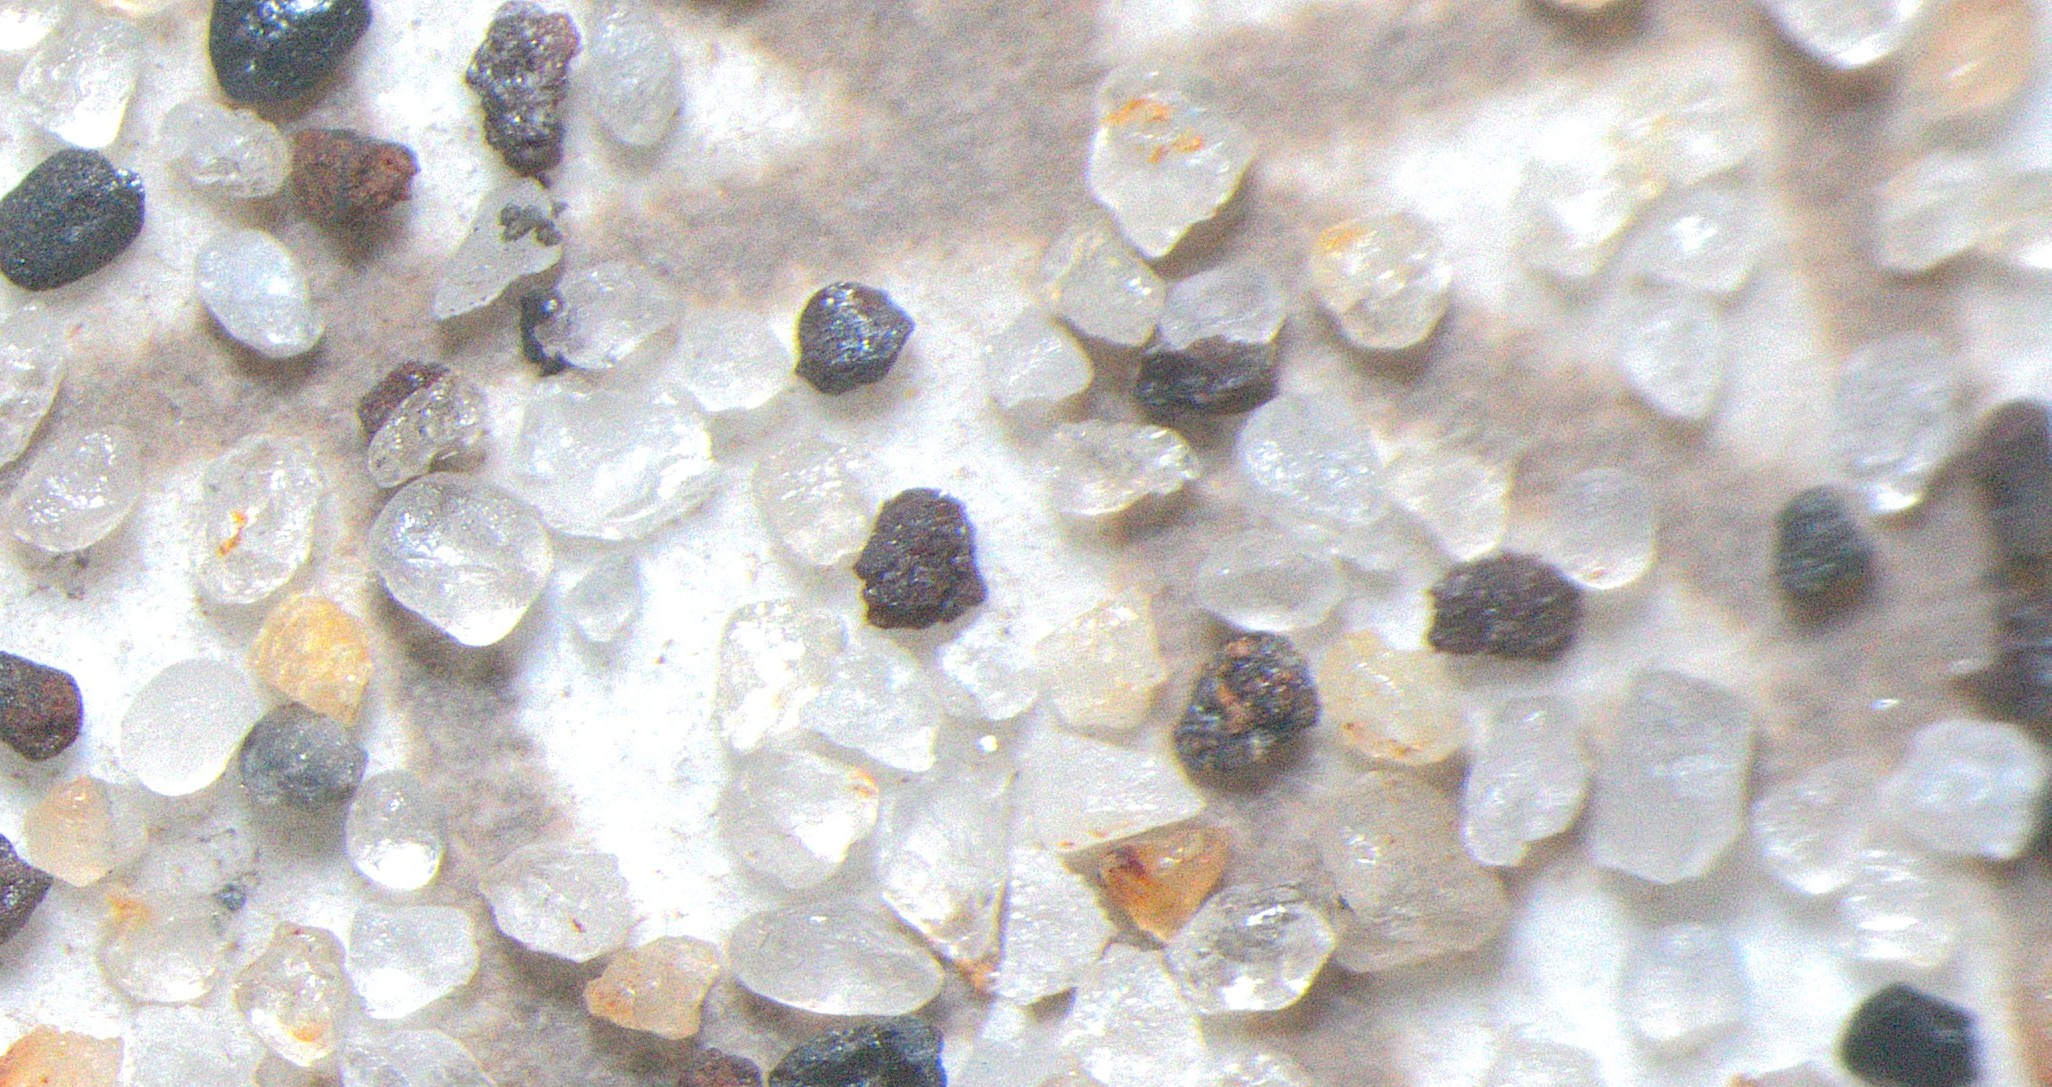
\includegraphics[width=4.05cm,height=4cm,keepaspectratio]{figure/pengujian/5/1347-20_48E_tile1.jpg}}} &
    \multirow{2}{*}{1} &

    10\rule{0pt}{3.0em} & 1 & 0 & 0 & 9 & 0 & 1{,}000 & 0{,}951 & 1 &
    V1 \textit{(Am)} \\

    \cline{4-13}

    & & &   % ← WAJIB: kosongkan No | Citra | GT Total
    11\rule{0pt}{3.0em} & 1 & 0 & 0 & 10 & 0 & 0{,}900 & \textit{NaN} & 1 &
    V2 \textit{(Std)} \\

    \hline

    % ===== Data ke-6 =====
    \multirow{2}{*}{6} &
    \multirow{2}{*}{%
    \parbox[c][1.5cm][c]{4cm}{%
    \centering
    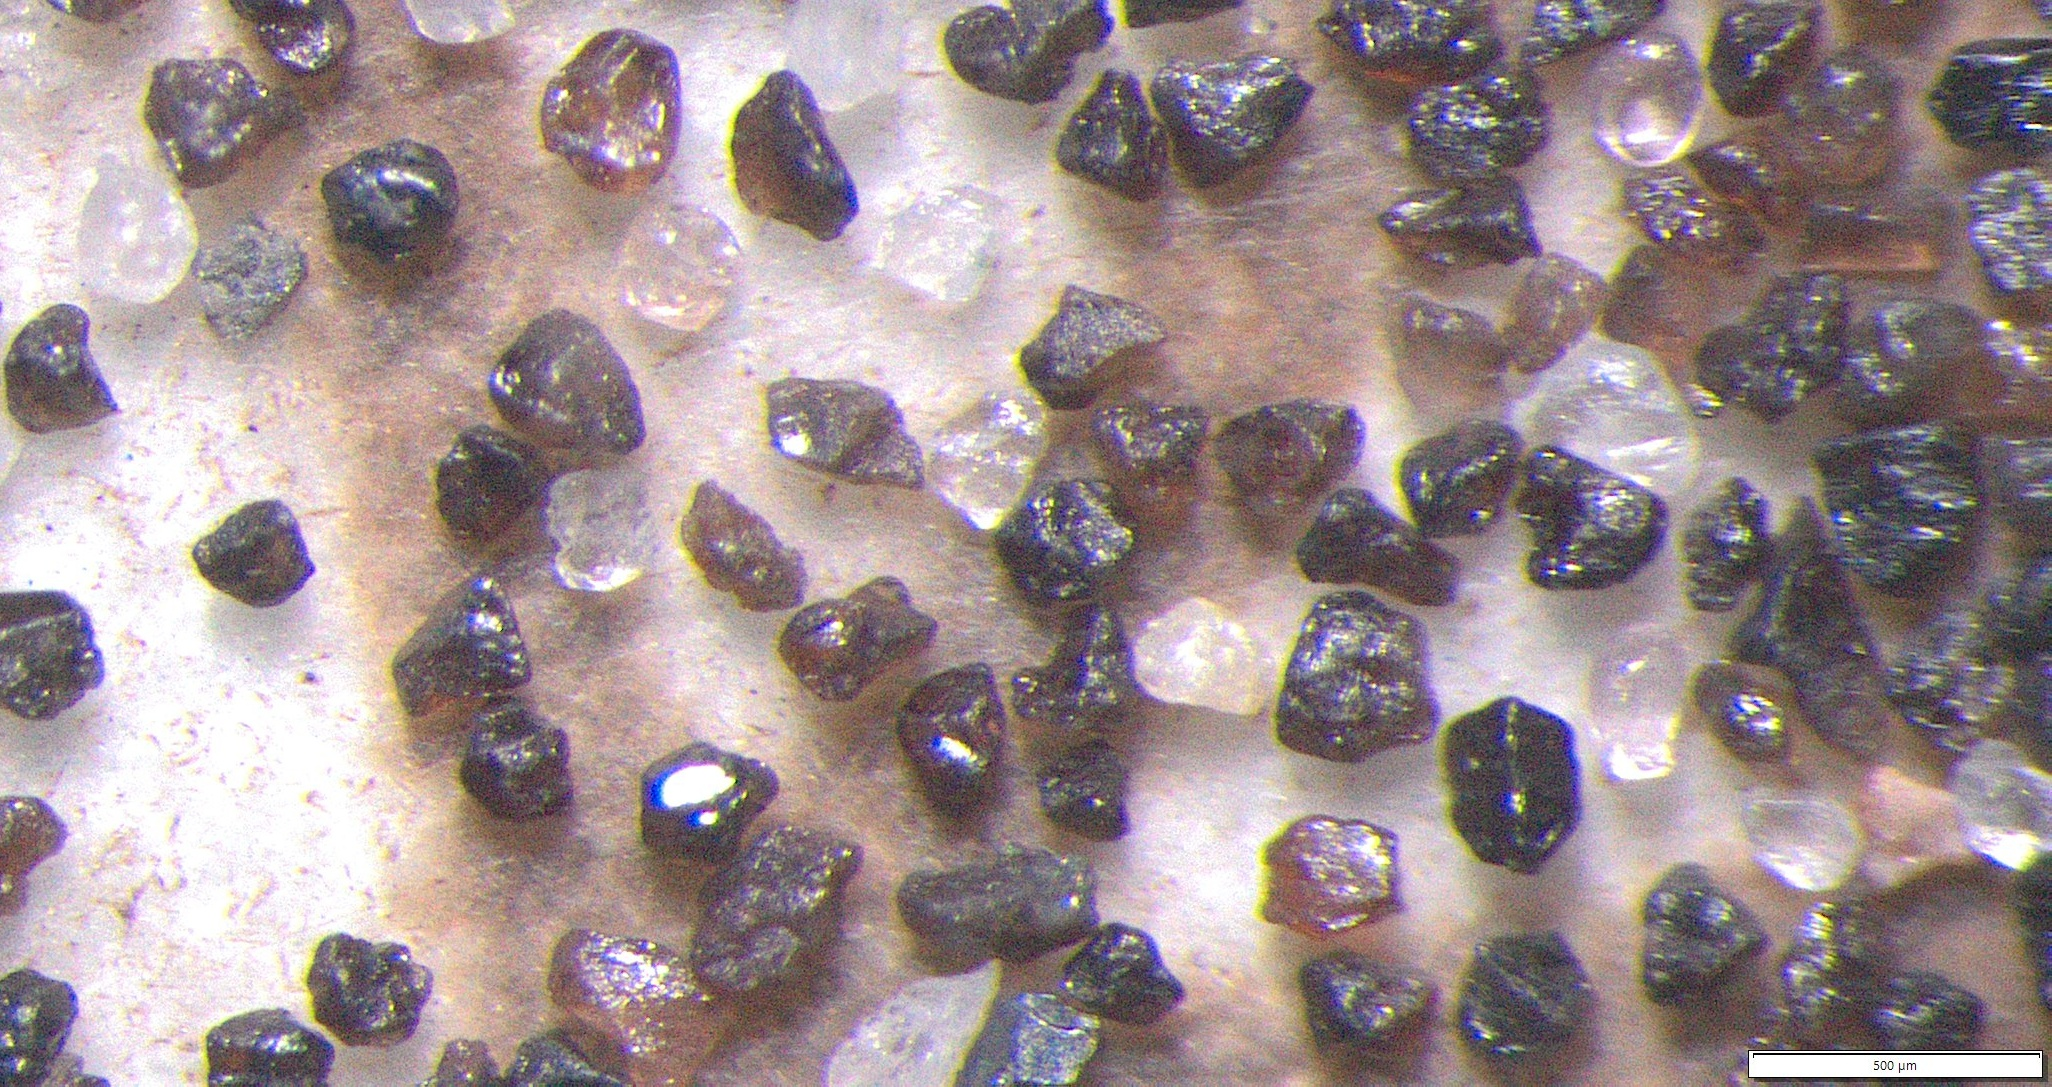
\includegraphics[width=4.05cm,height=4cm,keepaspectratio]{figure/pengujian/6/0384-16_100H_tile3.jpg}}} &
    \multirow{2}{*}{31} &

    46\rule{0pt}{3.0em} & 17 & 7 & 1 & 21 & 6 & 0{,}687 & 0{,}921 & 25 &
    V1 \textit{(Am)} \\

    \cline{4-13}

    & & &   % ← WAJIB: kosongkan No | Citra | GT Total
    71\rule{0pt}{3.0em} & 30 & 0 & 0 & 41 & 1 & 0{,}852 & 0{,}924 & 30 &
    V2 \textit{(Std)} \\

    \hline

\end{longtable}
\end{landscape}
\restoregeometry

Berdasarkan Tabel \ref{table:4.Pengujian1}, hasil pengujian menunjukkan perbedaan karakteristik antara kedua model berdasarkan beberapa kategori evaluasi deteksi. Model V2 \textit{Standard} mampu mengidentifikasi objek kasiterit dengan akurasi yang tinggi, sebagaimana tercermin dari nilai \APrangefiftyy dan \IoUrangefiftyy yang cukup baik. Namun, model ini cenderung melakukan \textit{overprediction}, yang mengakibatkan tingginya angka \textit{False Positive}. Selain itu, pada data uji ke-5, model V2 \textit{Standard} menghasilkan nilai \IoUrangefiftyy berupa \textit{NaN}, yang mengindikasikan kegagalan deteksi pada ambang batas IoU tertentu, khususnya pada IoU tinggi. Sebaliknya, model V1 \textit{Amodal} menunjukkan performa yang lebih baik dalam hal segmentasi, ditandai dengan nilai \IoUrangefiftyy yang lebih tinggi secara konsisten. Model ini juga lebih stabil dalam melakukan prediksi dan tidak mengalami \textit{overprediction} seperti model V2 \textit{Standard}, sehingga menghasilkan jumlah \textit{False Positive} yang lebih rendah. Namun, stabilitas tersebut berdampak pada nilai \APrangefiftyy yang cenderung lebih rendah dibandingkan model V2 \textit{Standard}, mengindikasikan bahwa model V1 \textit{Amodal} lebih konservatif dalam melakukan prediksi. \par

\begin{figure}[H]
    \centering
    % Baris pertama: dua gambar sejajar
    \begin{subfigure}[b]{0.475\textwidth}
        \centering
        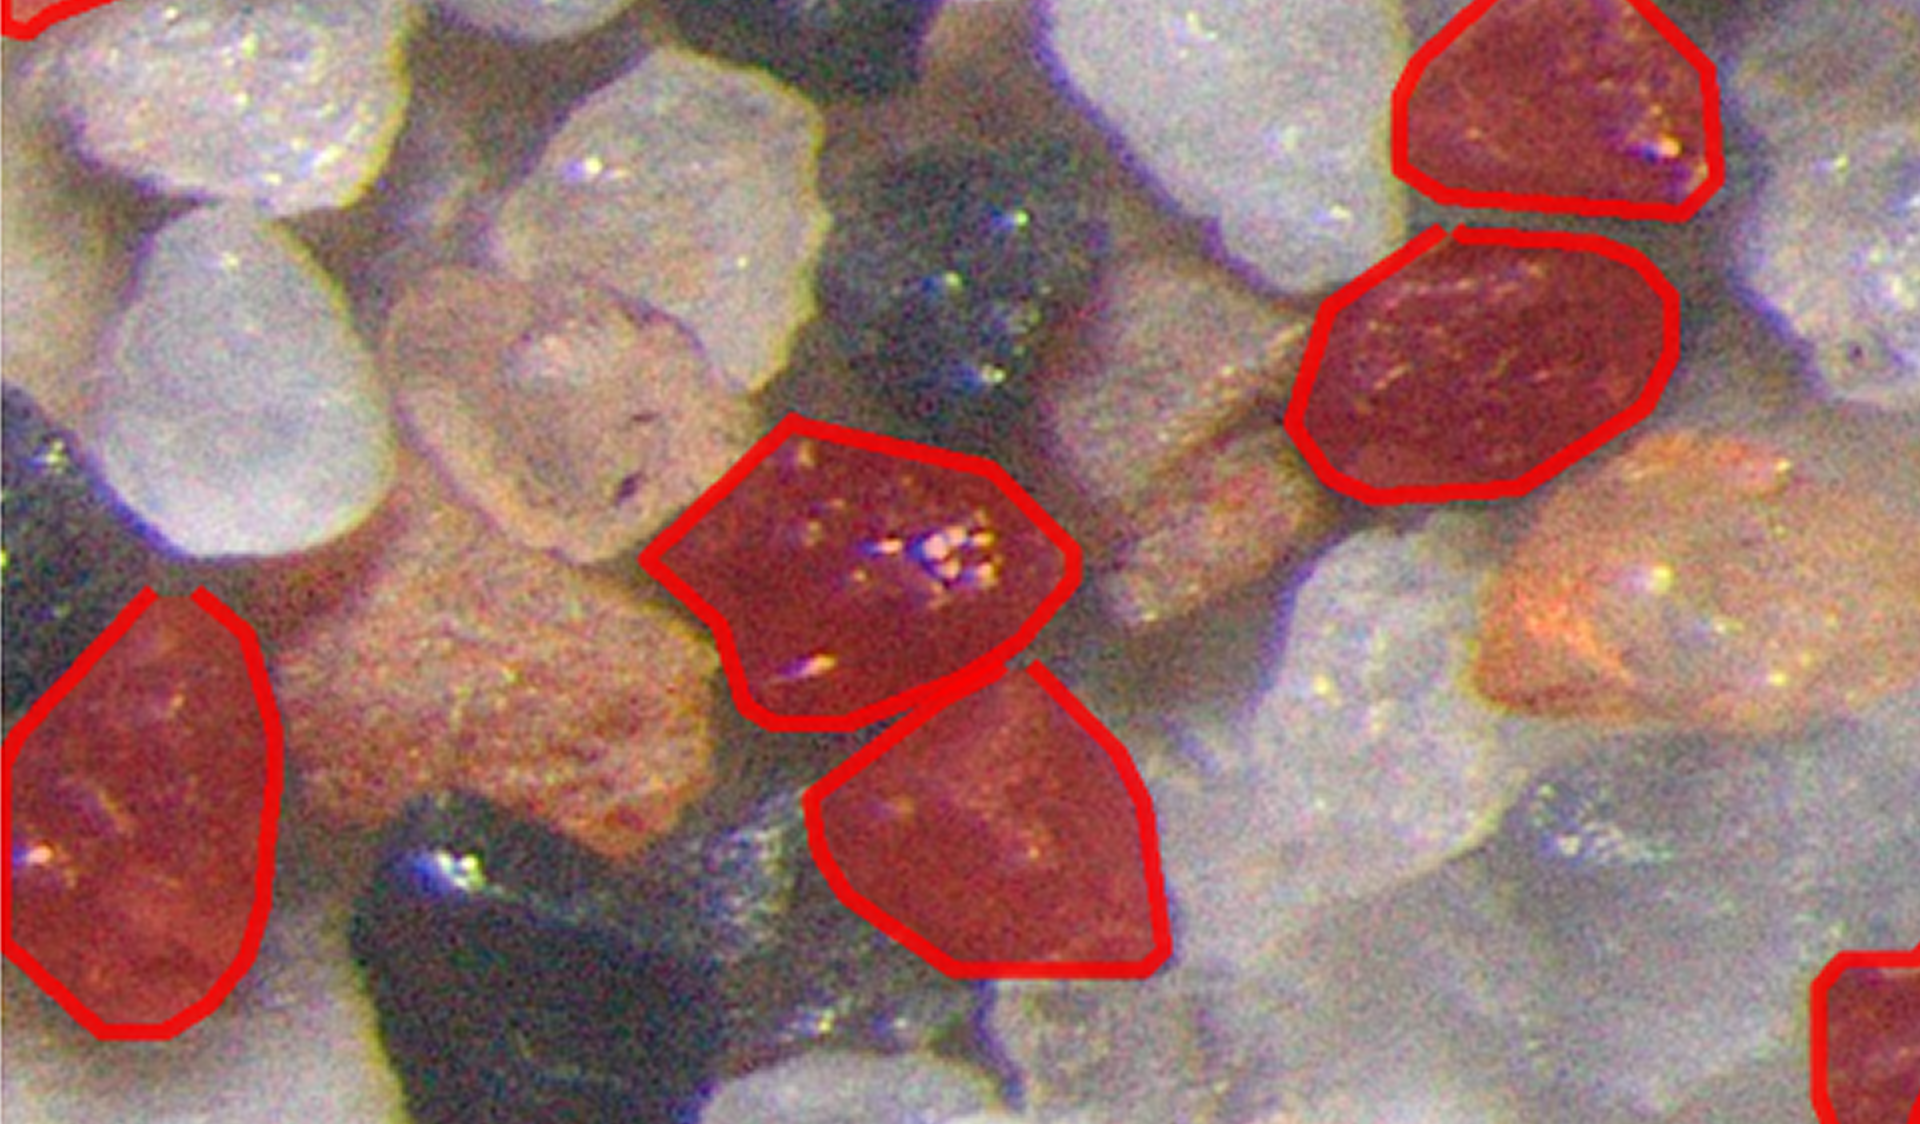
\includegraphics[width=\textwidth]{figure/oklusi/tile_2 - GT.png}
        \caption{Citra Ground Truth}
        \label{fig:4.Citra_gt}
    \end{subfigure}
    
    % Baris kedua: satu gambar di bawah tengah
    \vskip\baselineskip
    \begin{subfigure}[b]{0.475\textwidth}
        \centering
        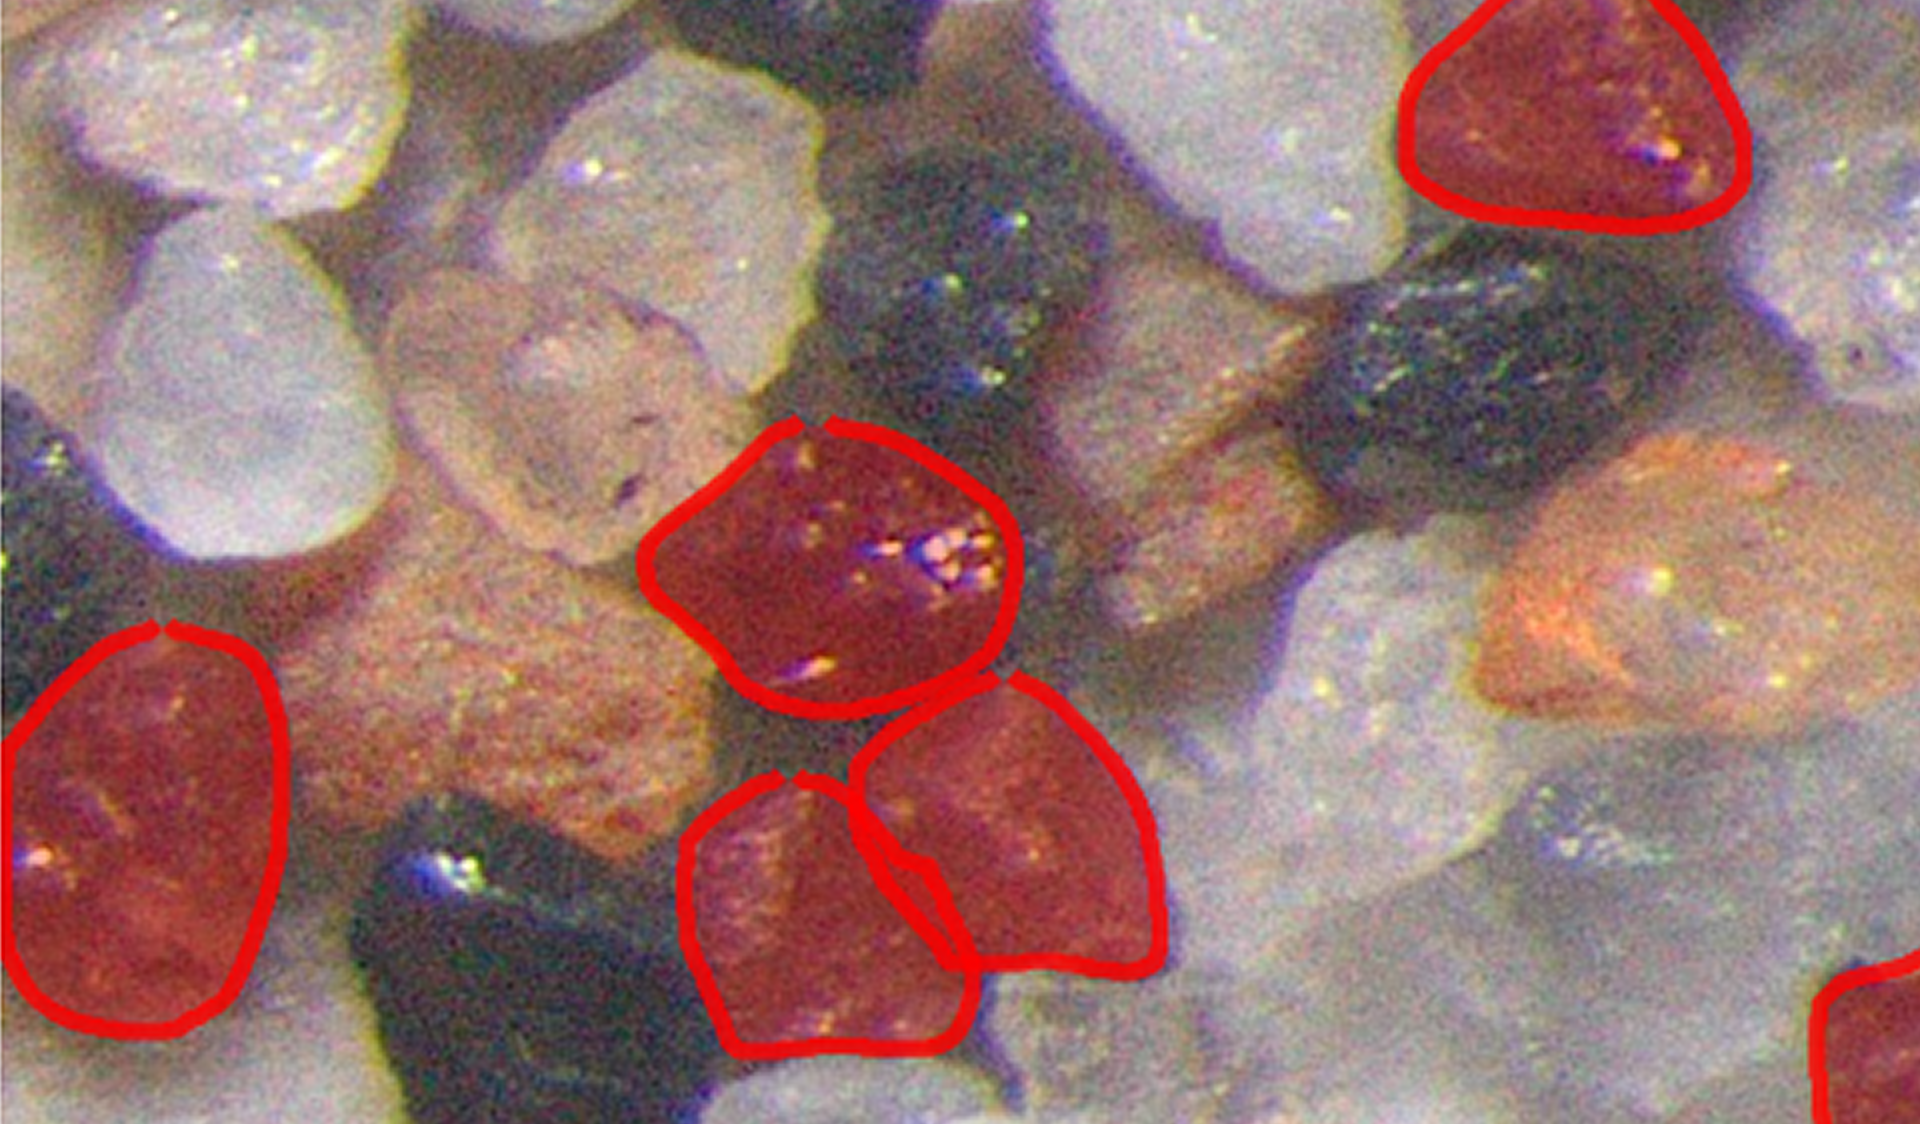
\includegraphics[width=\textwidth]{figure/oklusi/tile_2 - Amodal.png}
        \caption{Hasil Prediksi Model V1 \textit{Amodal} \textit{Adam}}
        \label{fig:4.hasil_amodal}
    \end{subfigure}
    \hfill
    \begin{subfigure}[b]{0.475\textwidth}
        \centering
        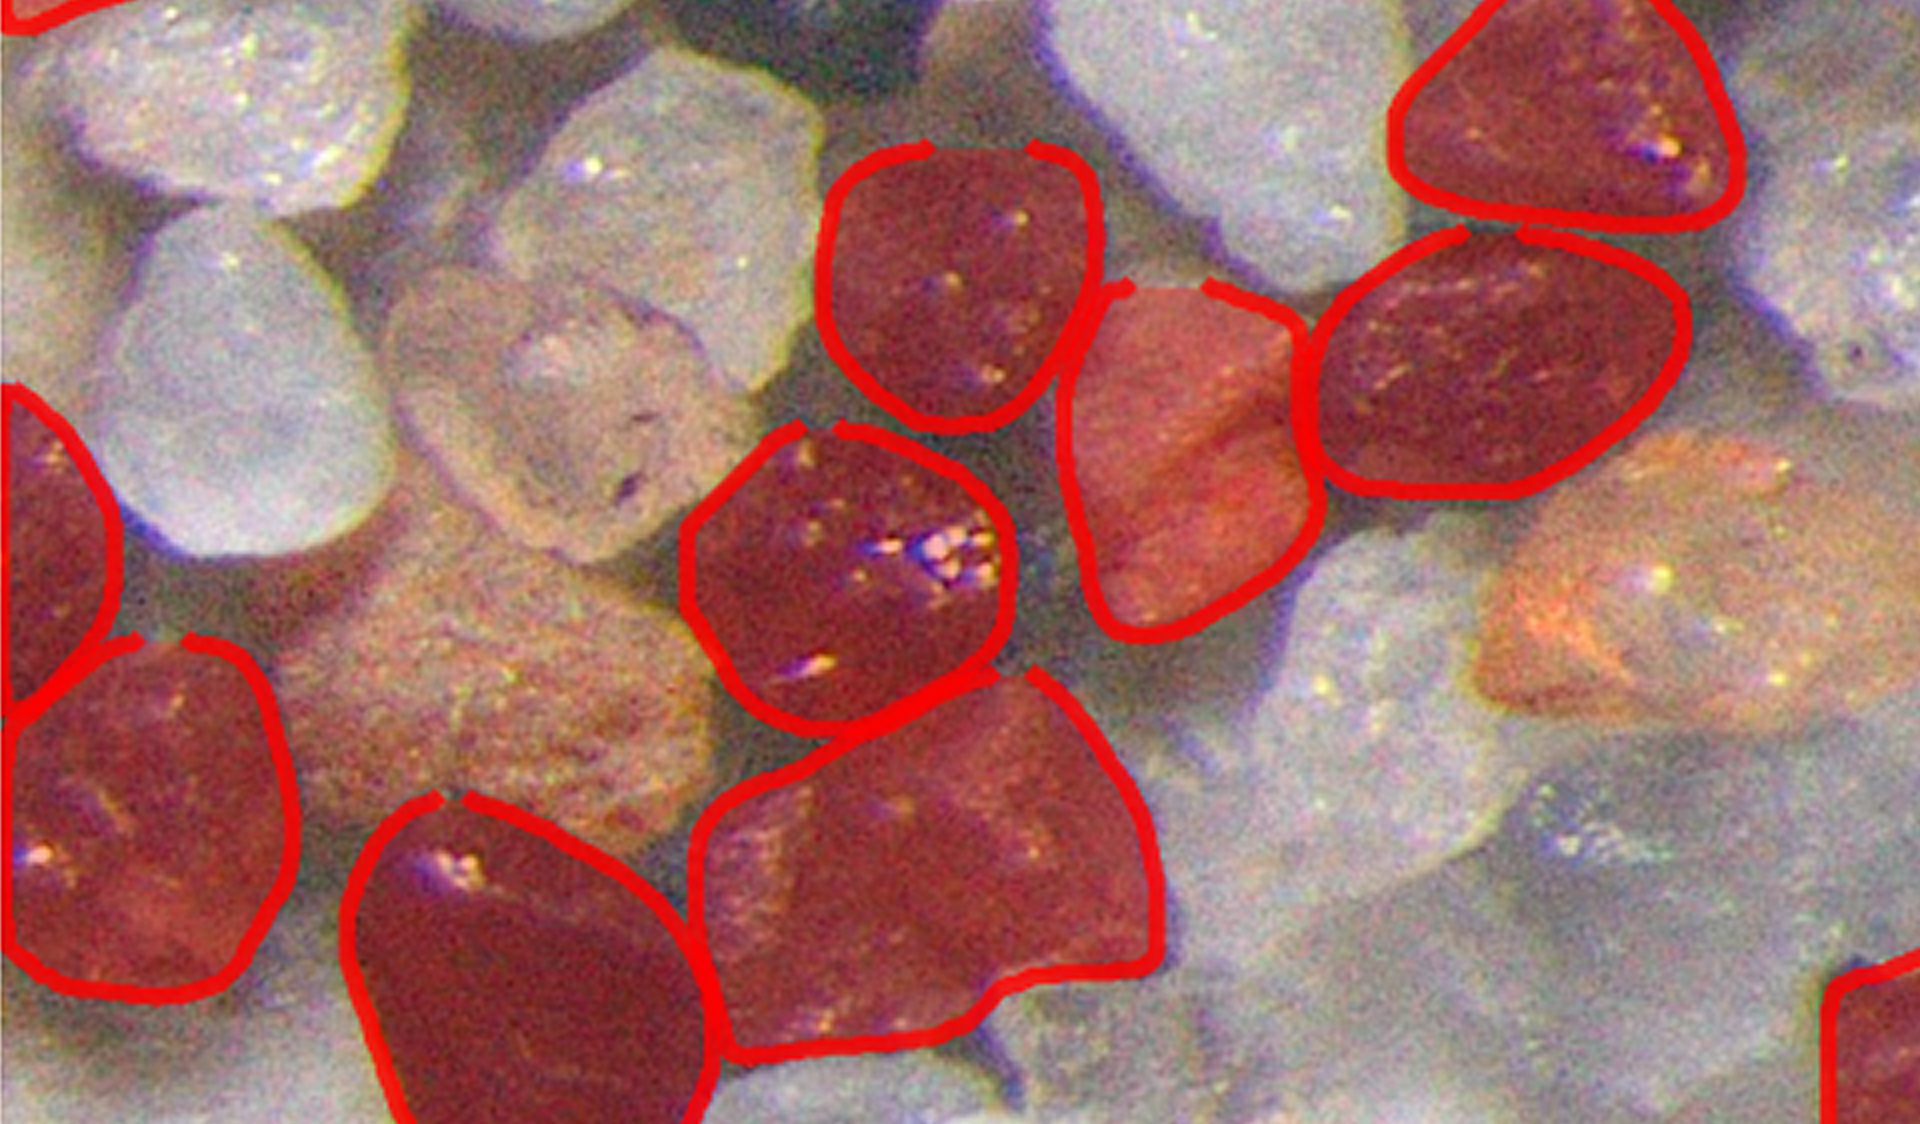
\includegraphics[width=\textwidth]{figure/oklusi/tile_2 - Standard.png}
        % \caption{Hasil \textit{Flip} Vertical ($\shortdownarrow$)}
        \caption{Hasil Prediksi Model V2 \textit{Standard} SGD}
        % \caption{Hasil \textit{Flip} Vertical ($\downarrow$)}

        \label{fig:4.hasil_stadard}
    \end{subfigure}
    \caption{Contoh Hasil Oklusi dengan Objek}
    \label{fig:4.Hasil_oklusi_dengan_objek}
\end{figure}

Berdasarkan pada Gambar \ref{fig:4.Hasil_oklusi_dengan_objek}, terlihat bahwa pada area kasiterit yang saling bersebelahan dan mengalami oklusi, model V1 \textit{Amodal} dengan \textit{optimizer Adam} mampu memisahkan dan memprediksi masing-masing butir kasiterit secara individual, meskipun sebagian bentuk objek tertutup oleh butir lain. Hal ini tampak dari beberapa area berwarna merah yang tetap tersegmentasi sebagai objek terpisah sesuai dengan anotasi \textit{Ground Truth}. Sebaliknya, pada hasil model V2 \textit{Standard} dengan \textit{optimizer} SGD, area kasiterit yang saling menutupi tersebut cenderung diprediksi sebagai satu objek utuh, sehingga batas antar butir yang berdekatan tidak terpisahkan dengan baik. Perbedaan ini menunjukkan bahwa pendekatan \textit{amodal} lebih efektif dalam menangani kondisi oklusi antar butir kasiterit dibandingkan pendekatan \textit{standard} yang bergantung pada area objek yang tampak secara visual.

\begin{figure}[H]
    \centering
    % Baris pertama: dua gambar sejajar
    \begin{subfigure}[b]{0.475\textwidth}
        \centering
        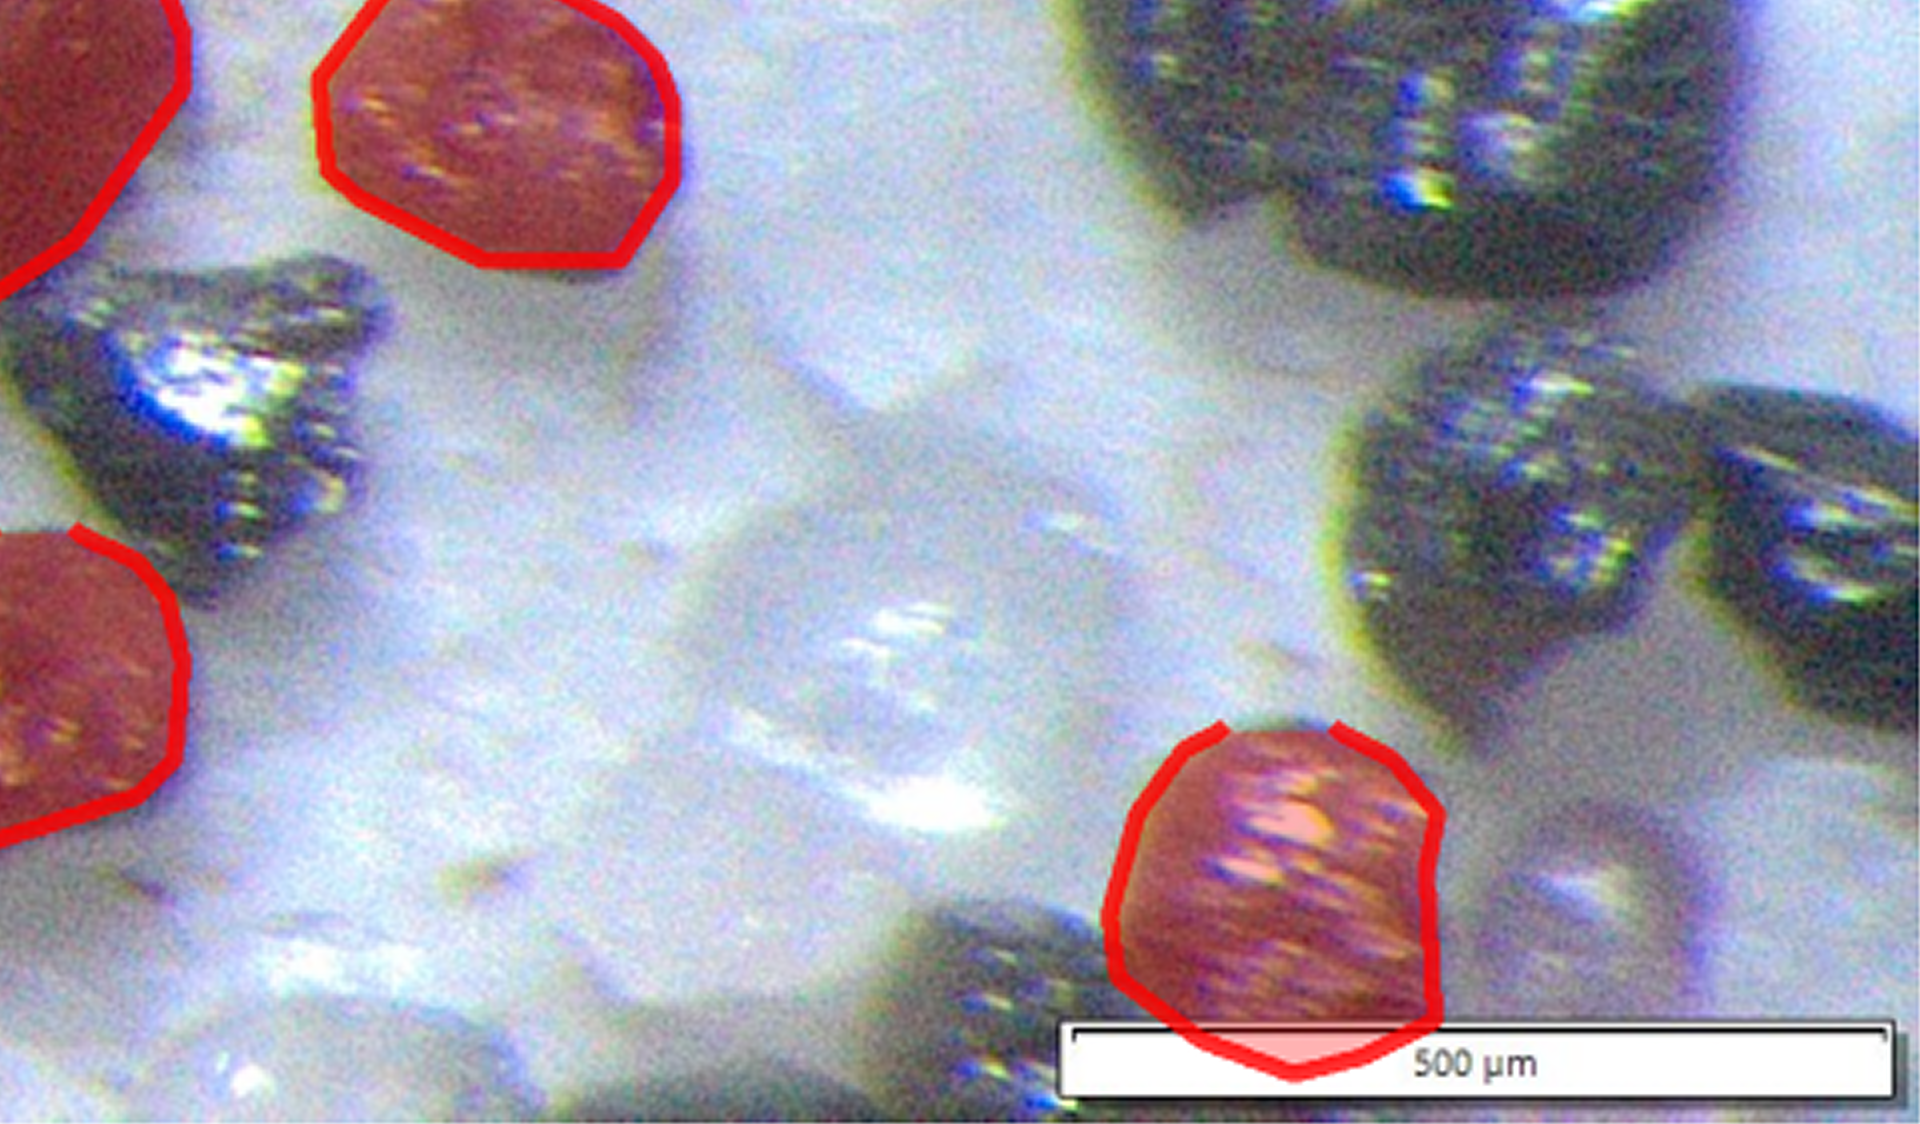
\includegraphics[width=\textwidth]{figure/oklusi/tile_4 - GT.png}
        \caption{Citra Ground Truth}
        \label{fig:4.Citra_gt1}
    \end{subfigure}
    
    % Baris kedua: satu gambar di bawah tengah
    \vskip\baselineskip
    \begin{subfigure}[b]{0.475\textwidth}
        \centering
        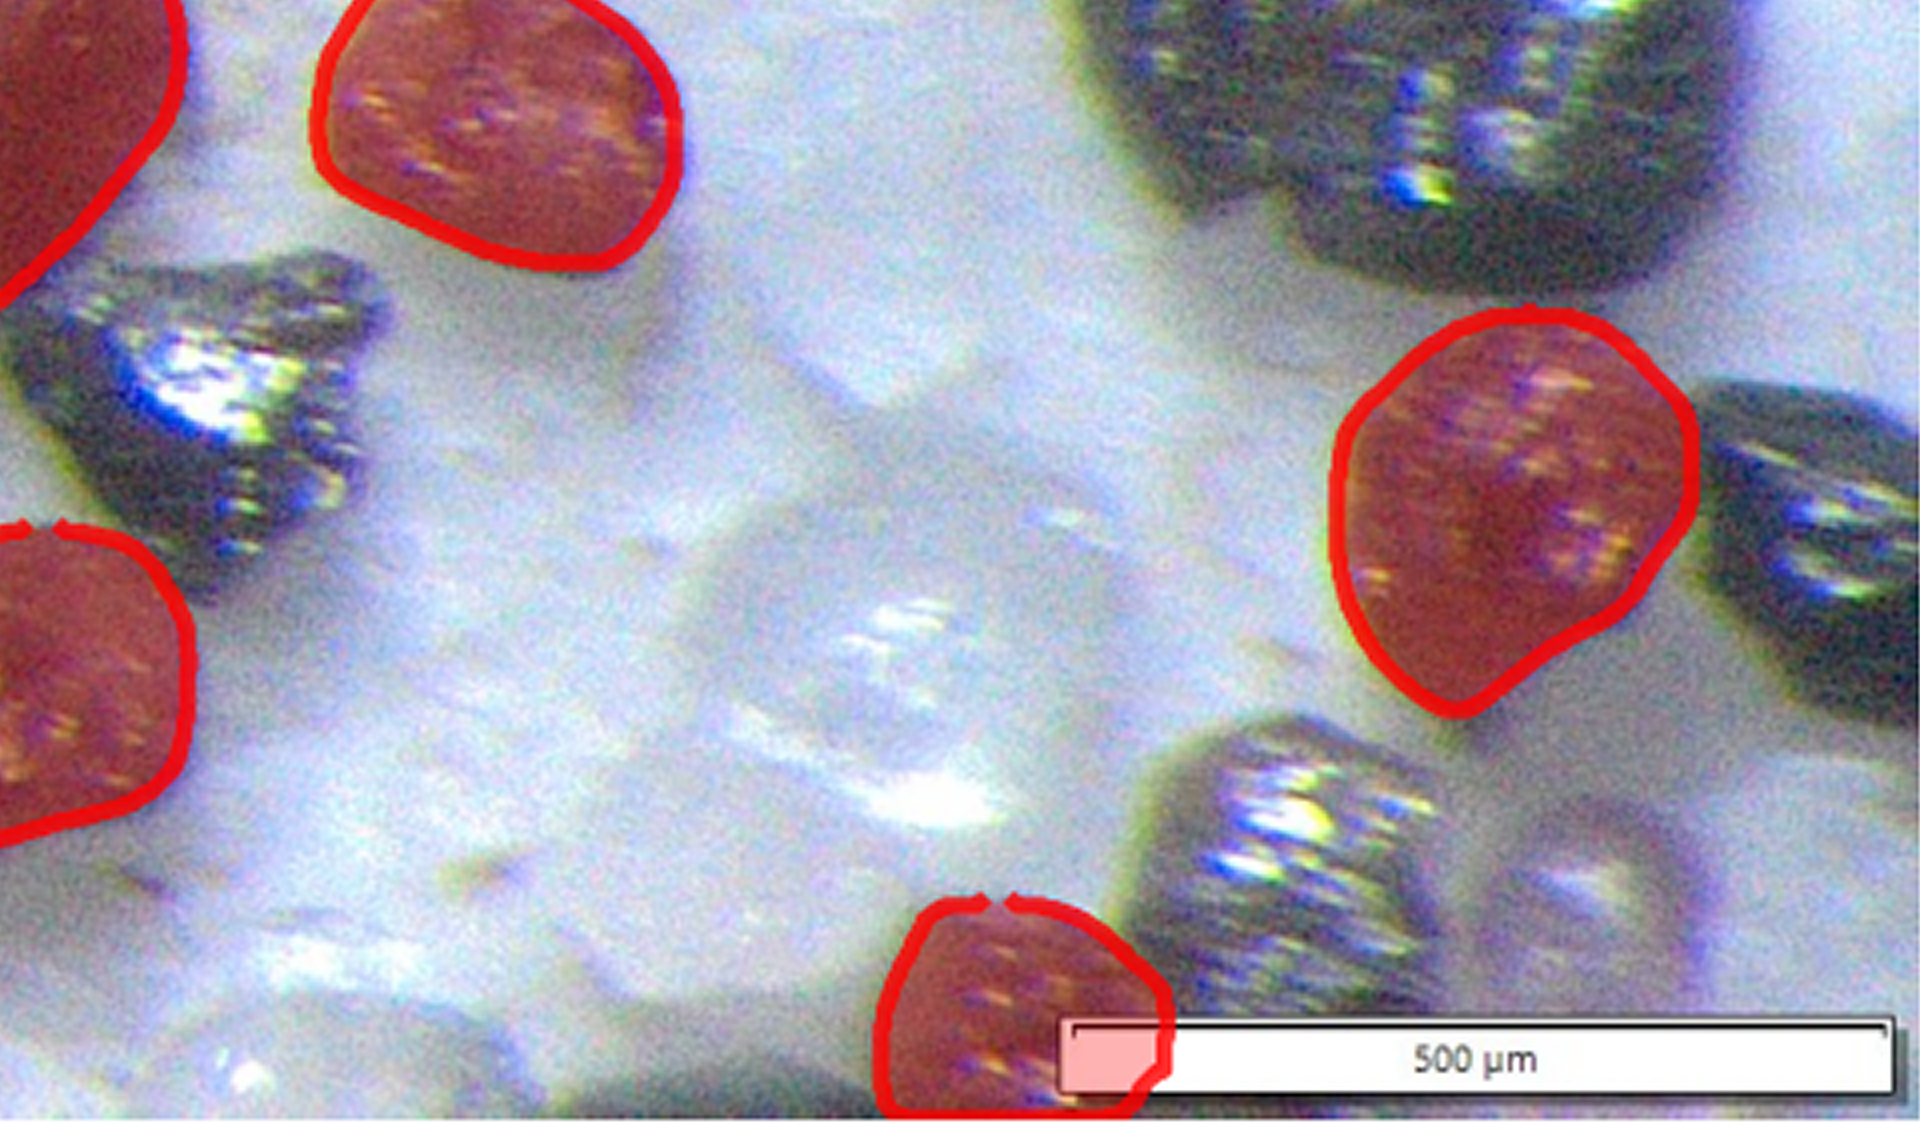
\includegraphics[width=\textwidth]{figure/oklusi/tile_4 - Amodal.png}
        \caption{Hasil Prediksi Model V1 \textit{Amodal} \textit{Adam}}
        \label{fig:4.hasil_amodal1}
    \end{subfigure}
    \hfill
    \begin{subfigure}[b]{0.475\textwidth}
        \centering
        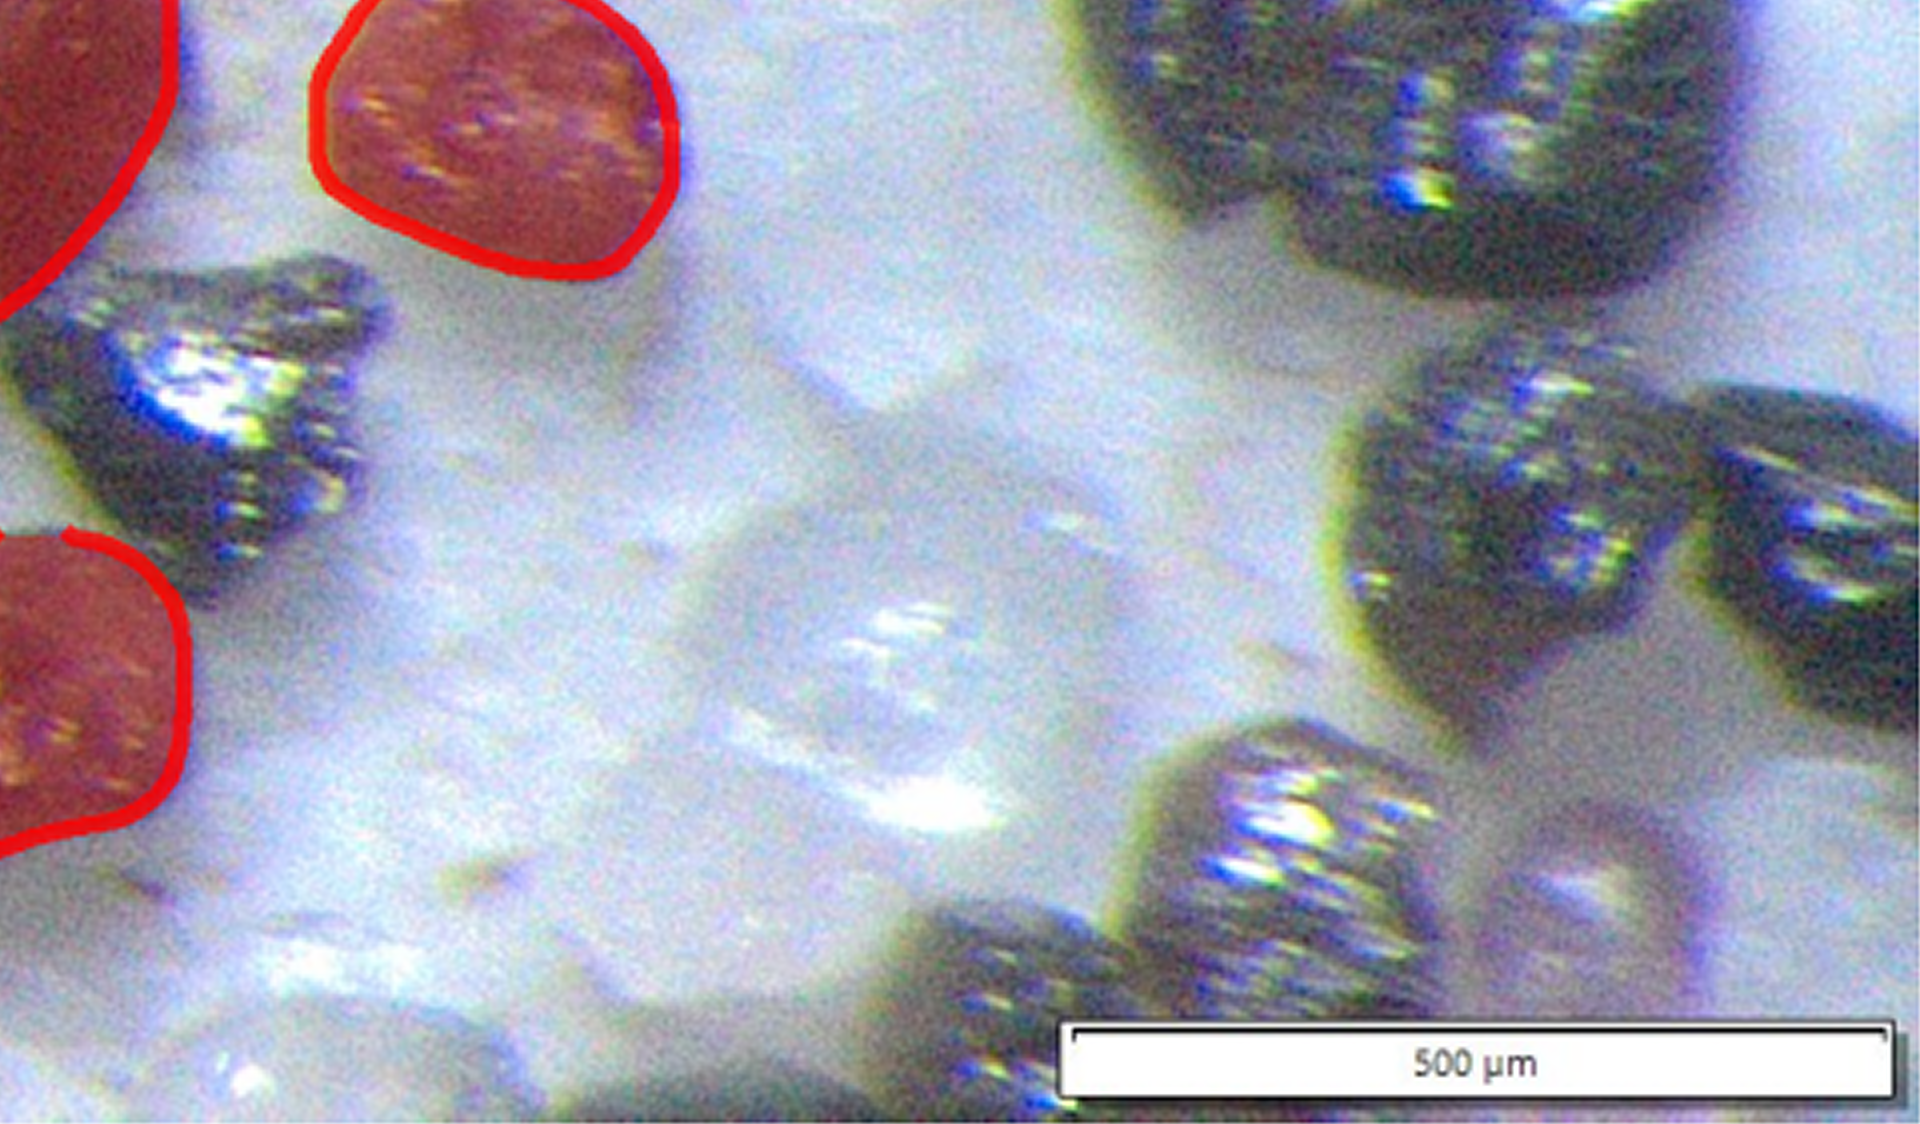
\includegraphics[width=\textwidth]{figure/oklusi/tile_4 - Standard.png}
        % \caption{Hasil \textit{Flip} Vertical ($\shortdownarrow$)}
        \caption{Hasil Prediksi Model V2 \textit{Standard} SGD}
        % \caption{Hasil \textit{Flip} Vertical ($\downarrow$)}

        \label{fig:4.hasil_stadard1}
    \end{subfigure}
    \caption{Contoh Hasil Oklusi dengan Background}
    \label{fig:4.Hasil_oklusi_dengan_bg}
\end{figure}

Berdasarkan pengamatan pada Gambar \ref{fig:4.Hasil_oklusi_dengan_bg}, terlihat bahwa pada bagian pojok kanan citra terdapat elemen latar belakang berupa penanda skala (500 $\mu$m) yang menutupi sebagian objek kasiterit. Pada kondisi ini, berdasarkan perbandingan dengan \textit{ground truth} yang berjumlah empat objek kasiterit, model V1 \textit{amodal} dengan \textit{optimizer} \textit{Adam} menghasilkan lima prediksi, dengan tiga objek terdeteksi dengan benar, satu objek tidak terdeteksi, serta dua prediksi yang termasuk kesalahan deteksi. Meskipun terdapat kesalahan, model V1 tetap mampu melakukan segmentasi pada salah satu objek kasiterit yang teroklusi oleh latar belakang, di mana area objek masih diprediksi meskipun sebagian tertutup elemen non-objek. Sebaliknya, model V2 \textit{standard} dengan \textit{optimizer} SGD hanya menghasilkan tiga deteksi yang benar dan satu objek tidak terdeteksi, serta tidak mampu melakukan segmentasi pada area yang mengalami oklusi sehingga tidak menghasilkan prediksi pada lokasi tersebut. Hal ini menunjukkan bahwa model \textit{amodal} memiliki kemampuan yang lebih baik dalam mengenali keberadaan kasiterit pada kondisi oklusi oleh latar belakang dibandingkan model \textit{standard} yang sangat bergantung pada visibilitas penuh objek. \par

\section{Analisis Hasil Keseluruhan} \label{IV.Analisis_Hasil_Keseluruhan}
Dalam penelitian ini, metrik \textit{Average Precision} pada rentang \textit{Intersection over Union} 0{,}50 hingga 0{,}95 (\APrangefifty) digunakan sebagai indikator utama dalam menentukan konfigurasi model terbaik karena mampu merepresentasikan kinerja model secara konsisten pada berbagai tingkat ambang \textit{IoU}. Metrik ini memberikan gambaran objektif mengenai akurasi deteksi dan presisi segmentasi model pada kondisi evaluasi yang bervariasi. Selain itu, metrik \IoUrangefiftyy digunakan untuk menilai tingkat kesesuaian segmentasi antara hasil prediksi dan \textit{ground truth}. Kombinasi kedua metrik tersebut memungkinkan evaluasi performa model yang lebih komprehensif dan terukur. \par

Pada hasil percobaan dari variasi konfigurasi pelatihan model terbaik pada \textit{Mask} R-CNN ResNet50 FPN V1 dan V2, didapatkan bahwa model \textit{pre-trained} \textit{Mask} R-CNN ResNet50 FPN V1 dengan variasi model \textit{Amodal} dan \textit{optimizer} \textit{Adam} menunjukkan performa terbaik dengan nilai \textit{AP50:95} sebesar 0{,}458 dan \textit{IoU50:95} sebesar 0{,}915. Model \textit{pre-trained} \textit{Mask} R-CNN ResNet50 FPN V2 dengan variasi model \textit{Standard} dan \textit{optimizer} SGD menunjukkan performa yang sedikit lebih rendah dengan nilai \textit{AP50:95} sebesar 0{,}449 dan \textit{IoU50:95} sebesar 0{,}915. Nilai tersebut memiliki selisih nilai \textit{AP50:95} sebesar 0{,}009 (0{,}9\%) dan nilai \textit{IoU50:95} sama, yang menunjukkan variasi model V1 \textit{Amodal} lebih unggul dibandingkan variasi model V2 \textit{Standard}.  \par

Penerapan teknik \textit{Amodal Instance Segmentation} menunjukkan pengaruh yang berbeda-beda pada kinerja model \textit{Mask} R-CNN. Pada model \textit{pre-trained} Mask R-CNN ResNet50 FPN V1 dengan \textit{optimizer} Adam, penambahan pendekatan \textit{amodal} yang meningkatkan jumlah parameter sebesar 2.950.914 (6{,}75\%) mampu meningkatkan performa, ditunjukkan oleh kenaikan nilai \textit{AP50:95} dari 0{,}437 menjadi 0{,}458 serta peningkatan \textit{IoU50:95} dari 0{,}910 menjadi 0{,}915, dengan tambahan waktu pelatihan sebesar 0{,}37 jam. Sebaliknya, pada model \textit{pre-trained} Mask R-CNN ResNet50 FPN V2 dengan \textit{optimizer} SGD, penerapan teknik \textit{amodal} yang menambah parameter sebesar 2.950.914 (6{,}46\%) justru menurunkan performa, dengan nilai \textit{AP50:95} berkurang dari 0{,}449 menjadi 0{,}420 dan \textit{IoU50:95} dari 0{,}915 menjadi 0{,}913, meskipun waktu pelatihan hanya bertambah 0{,}45 jam. Hasil ini menunjukkan bahwa peningkatan kompleksitas melalui pendekatan \textit{amodal} tidak selalu berbanding lurus dengan peningkatan kinerja, serta sangat bergantung pada arsitektur \textit{pre-trained} dan pemilihan \textit{optimizer}. \par

Dari segi efisiensi parameter, peningkatan kompleksitas model tidak selalu berbanding lurus dengan peningkatan efisiensi parameter. Model \textit{Mask} R-CNN ResNet50 FPN V1 \textit{Standard} dengan \textit{optimizer} SGD menunjukkan efisiensi parameter tertinggi dengan total 43{,}699{,}995 parameter serta rasio \textit{AP/Param} sebesar $9{,}999\times10^{-9}$ dan \textit{IoU/Param} sebesar $2{,}082\times10^{-8}$. Penerapan pendekatan \textit{amodal} pada V1 meningkatkan jumlah parameter menjadi 46{,}650{,}909, namun justru menurunkan efisiensi rasio kinerja terhadap parameter. Pola serupa juga terlihat pada varian V2, di mana model \textit{Standard} dengan \textit{optimizer} SGD (\textit{Param Ratio} 1{,}045$\times$) menunjukkan keseimbangan yang lebih baik dibandingkan model V2 \textit{Amodal} (\textit{Param Ratio} 1{,}113$\times$). Dengan demikian, meskipun pendekatan \textit{amodal} unggul dalam menangani oklusi, model \textit{Standard} khususnya pada varian V2 lebih sesuai untuk penerapan praktis segmentasi mineral kasiterit dari sisi efisiensi dan stabilitas kinerja. \par

Hasil pengujian menunjukkan adanya perbedaan karakteristik yang jelas antara kedua model. Model V2 \textit{standard} mampu mengidentifikasi objek kasiterit dengan akurasi yang tinggi, sebagaimana ditunjukkan oleh nilai \APrangefiftyy dan \IoUrangefiftyy yang relatif baik, namun cenderung mengalami \textit{overprediction} sehingga menghasilkan jumlah \textit{False Positive} yang lebih tinggi. Kondisi ini semakin terlihat pada data uji ke-5, di mana model V2 \textit{standard} menghasilkan nilai \IoUrangefiftyy berupa NaN, yang mengindikasikan kegagalan deteksi pada ambang batas IoU tertentu, khususnya pada IoU tinggi. Sebaliknya, model V1 \textit{amodal} menunjukkan performa segmentasi yang lebih stabil dan konsisten dengan nilai \IoUrangefiftyy yang lebih tinggi, serta tidak mengalami \textit{overprediction}, sehingga jumlah \textit{False Positive} yang dihasilkan lebih rendah. Namun, stabilitas dan sifat prediksi yang lebih konservatif tersebut berdampak pada nilai \APrangefiftyy yang cenderung lebih rendah dibandingkan model V2 \textit{standard}. \par

Hasil pengamatan pada contoh oklusi antar kasiterit dan oklusi dengan latar belakang, dapat dilihat bahwa model V1 \textit{Amodal} dengan \textit{optimizer} \textit{Adam} menunjukkan kemampuan yang lebih baik dalam mendeteksi objek kasiterit pada kondisi oklusi. Pada kasus kasiterit yang saling bersebelahan, model amodal mampu memisahkan dan memprediksi masing-masing butir kasiterit secara individual meskipun sebagian objek tertutup, sehingga hasil segmentasi tetap sesuai dengan anotasi \textit{Ground Truth}. Selain itu, pada kondisi oklusi oleh elemen latar belakang berupa penanda skala, model amodal masih mampu mendeteksi keberadaan kasiterit yang tertutup sebagian oleh \textit{background}. Sebaliknya, model V2 \textit{Standard} dengan \textit{optimizer} SGD cenderung memprediksi area kasiterit yang saling menutupi sebagai satu objek utuh serta gagal mendeteksi kasiterit yang teroklusi oleh latar belakang. Hasil ini menunjukkan bahwa pendekatan \textit{amodal} lebih efektif dalam menangani berbagai jenis oklusi, baik antar objek maupun dengan latar belakang. \par

Secara keseluruhan, hasil komparasi menunjukkan bahwa model \textit{pre-trained} \textit{Mask} R-CNN ResNet50 FPN V1 dengan pendekatan \textit{Amodal} dan \textit{optimizer} \textit{Adam} memberikan performa segmentasi yang lebih stabil dan unggul dalam menangani kondisi oklusi, ditunjukkan oleh nilai \textit{AP50:95} yang sedikit lebih tinggi, \textit{IoU50:95} yang konsisten, serta kemampuan mendeteksi objek kasiterit yang tertutup sebagian baik oleh objek lain maupun latar belakang. Sebaliknya, model \textit{Mask} R-CNN ResNet50 FPN V2 \textit{Standard} dengan \textit{optimizer} SGD memiliki efisiensi parameter yang lebih baik dan akurasi deteksi yang kompetitif, namun cenderung menghasilkan \textit{overprediction} dan menunjukkan keterbatasan dalam melakukan segmentasi pada objek yang mengalami oklusi. Dengan demikian, model V1 \textit{Amodal} lebih sesuai untuk skenario analisis citra mikroskop yang kompleks dan beroklusi, sedangkan model V2 \textit{Standard} lebih optimal dari sisi efisiensi dan stabilitas komputasi untuk penerapan praktis dengan kebutuhan sumber daya yang lebih terbatas. \par

% , dibandingkan pendekatan \textit{standard} yang lebih bergantung pada visibilitas visual objek. \par
